\documentclass{article}

%PACKAGES
\usepackage[utf8]{inputenc}
\usepackage[sorting=nty]{biblatex}
\usepackage{graphicx}
\graphicspath{ {./Figures/} }
\usepackage{amsmath} % \vspace{} \hspace{}
\usepackage{physics}
\usepackage[a4paper, margin=3cm]{geometry}
\usepackage{textpos} % plaats vakje voor figures
\usepackage{float} % Voor H! gebruik in figures
\usepackage{caption} 
\usepackage{changepage} % Changes table to left
\usepackage{comment}% Includes \begin{comment}
\usepackage{fancyhdr}
\usepackage{url}
\pagestyle{fancy}
\usepackage{xcolor} % colorpackage
\usepackage[colorlinks,linkcolor=black, citecolor=teal,urlcolor=blue]{hyperref} % hyperlinks citations
\usepackage{amssymb} % Expected symbol (\mathbb{E})
\usepackage{algorithm} % implement algorithm pseudocode
\usepackage{subcaption} % For multiple images
% \usepackage{subfigure}
\usepackage{bm} % For \boldsymbol
\usepackage{amsmath}
\usepackage[noend]{algpseudocode}
\usepackage{setspace}

\addbibresource{bib.bib}

\counterwithin{figure}{section}
%NEW COMMANDS
\newcommand{\eg}{e.\,g.\ }
\newcommand{\ie}{i.\,e.\ }

\newcommand{\WeightVector}{\overset{\rightarrow}{\boldsymbol{\theta}} }

\onehalfspacing

%BEGIN DOCUMENT
\begin{document}
% \nocite{*} % dont order citations

\thispagestyle{empty} 
\begin{center}
    \vspace*{0.5cm}
    \huge
    \textbf{Solving The Art Gallery Problem Using Gradient Descent}

    \vspace*{0.4cm}
    \LARGE
    \textbf{Master's Thesis}
    \vspace*{2cm}

    \begin{figure}[H]
        \centering   
        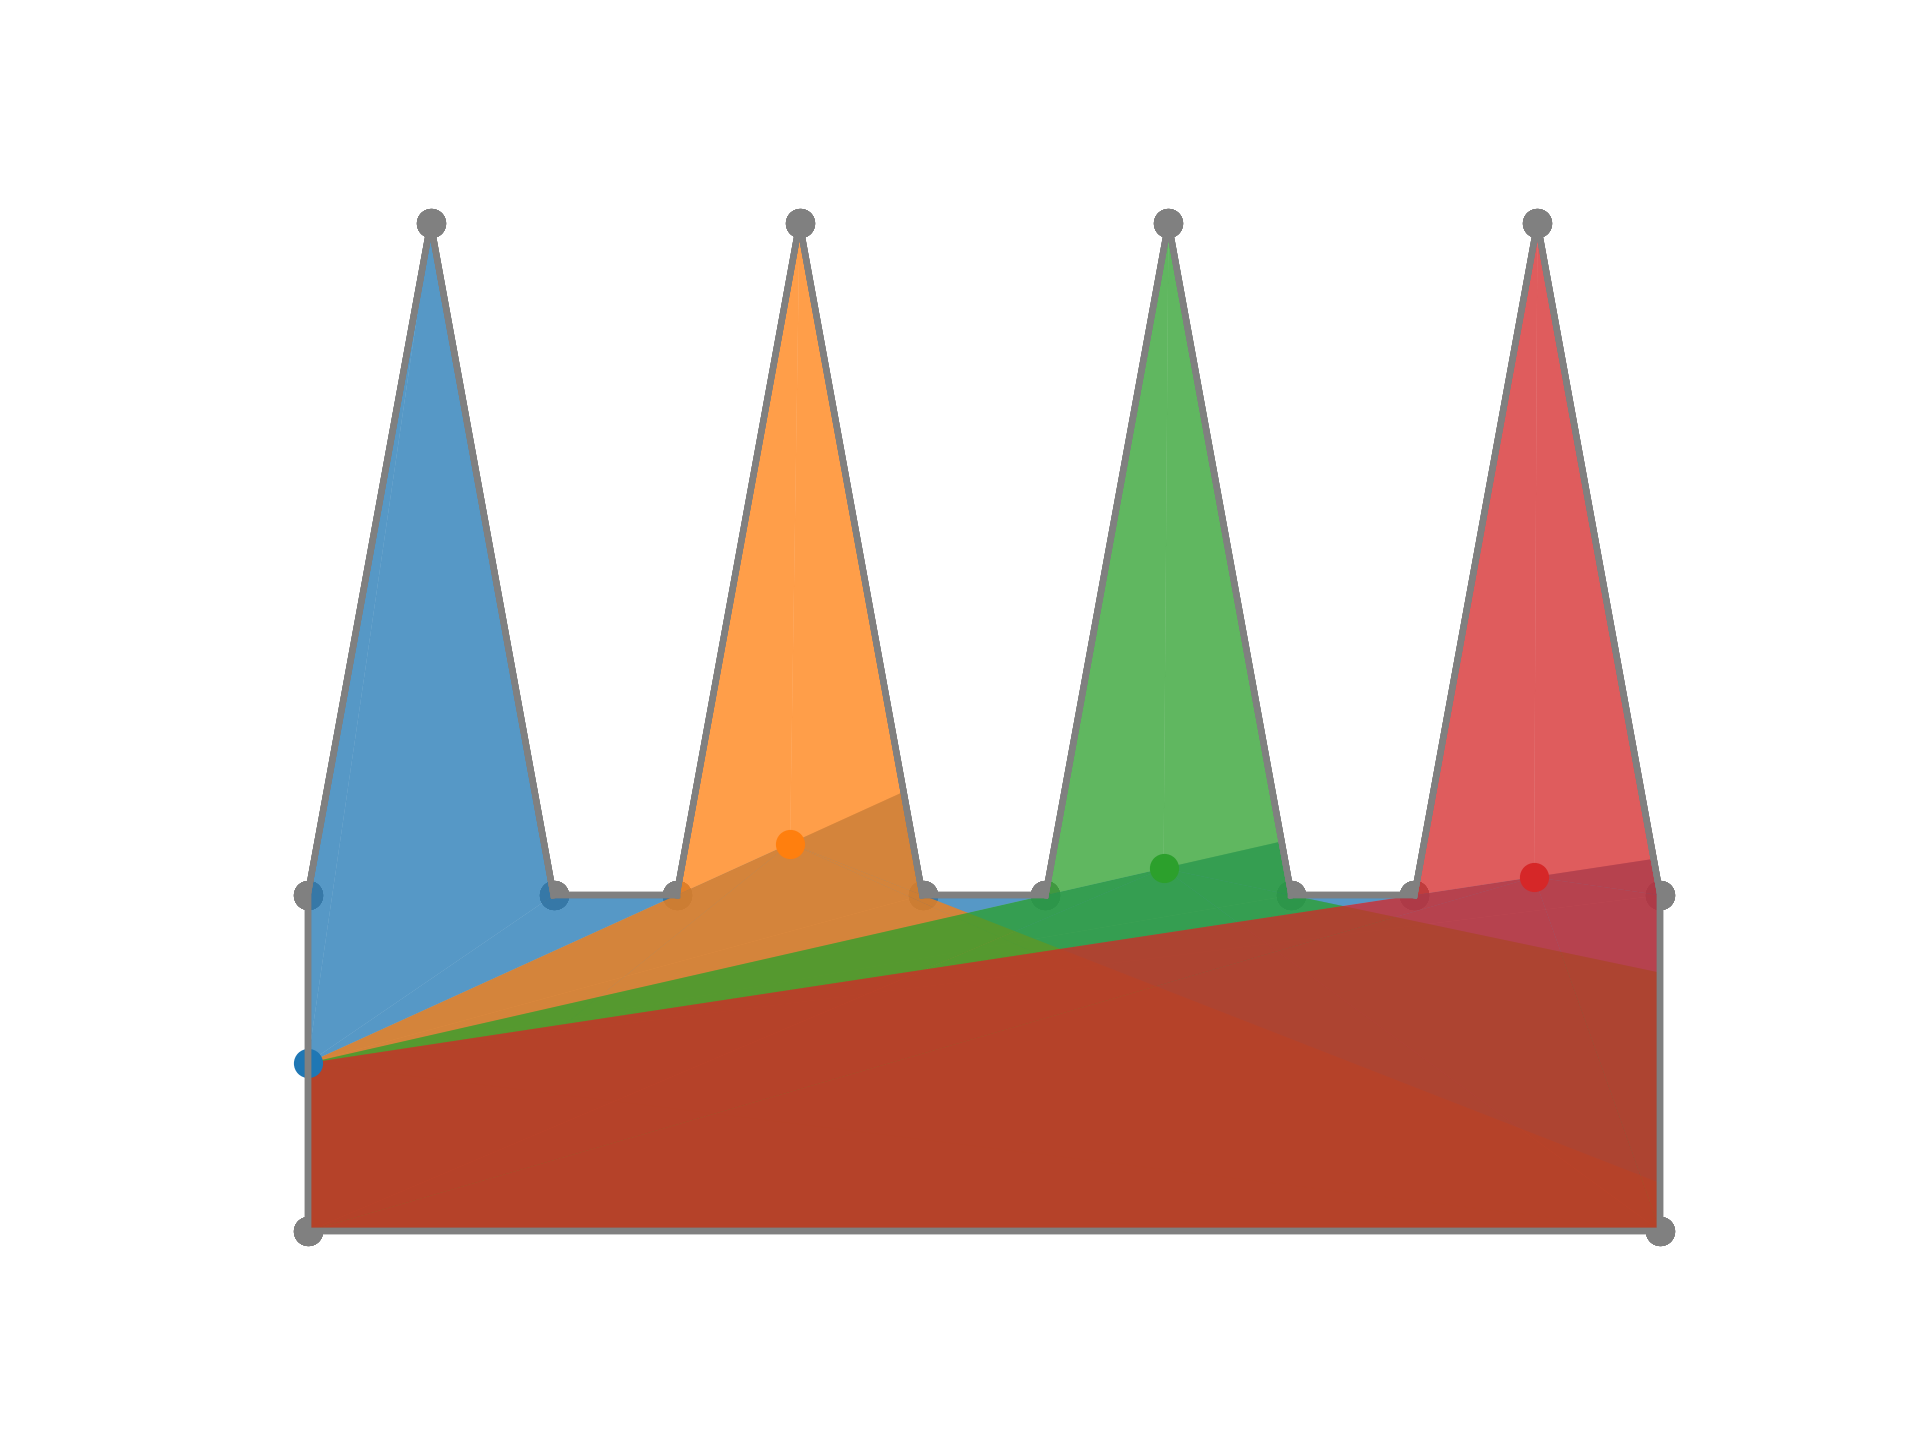
\includegraphics[width = 11cm]{comb_title.png}
    \end{figure}

    % Req indent

    \vspace{-1cm}
    \LARGE
    Georgiana Juglan
    \vfill 
    \large    
    \textbf{Supervisor:} \\
    Tillmann Miltzow \\
    \textbf{Second Examiner:} \\
    Frank Staals \\
     
\end{center}
   

\begin{textblock}{3}(6.5,0.7)

\includegraphics[width = 6cm]{Figures/UU logo.png}
\end{textblock}

\begin{flushleft}
    \vspace{0.5cm}
    % Master's Thesis \\
    Computing Science\\
    \today\\
    Student Nr. 2996307 \\
    Utrecht University\\
    The Netherlands
\end{flushleft}

\newpage
\thispagestyle{empty}
\section*{Abstract}

% In this thesis, machine learning agents learn to play the online browser game \href{https://Slither.io}{Slither.io}. In \textit{Slither} you play as a snake where the goal is to grow, by killing other snakes and eating food pellets. There are over 100 snakes in a single arena, and every player competes against each other under the same circumstances. The game has simple rules and controls, and yet complicated situations constantly emerge. The agents are trained with multiple machine learning methods such as imitation learning and deep Q-learning. Actor-critic policy gradient methods like PPO and SAC are given special attention, as they have the greatest potential in training agents that achieve superhuman performance. If time allows, the more complicated model-based methods are explored. The agents can observe their environment in different ways. For example by passing visual images through a CNN. This training and observing is established with an in-house replica of Slither in the game-engine Unity. Unity uses an API for communication with Python's machine learning library PyTorch to implement the machine learning algorithms. The main goal of this thesis is to create a superhuman player in Slither which can be deployed onto the original browser game.  Additionally, the aim is to compare the performance of different algorithms and techniques, to better understand how to effectively and efficiently train agents on competitive video games.

The Art Gallery Problem is one of the central problems in computational geometry. It was recently shown that the problem is $\exists \mathbb{R}$-complete. Thus it is unlikely to be solvable by methods that are usually applied to NP-complete problems. These methods include heuristics with provable guarantees to come as close as possible to the optimal solution in polynomial time. Nonetheless, one of the most important methods to solve $\exists \mathbb{R}$-complete problems is called gradient descent. Curiously, there was no attempt yet to solve the Art Gallery Problem by gradient descent. By aiming to maximise the area seen by the guards in the Art Gallery Problem, we get a continuous cost function, which allows us to compute a gradient. Using the gradient and other heuristics inspired from neural networks, we will try to solve the Art Gallery Problem practically using gradient descent. Specifically, we aim to use the library CGAL. 
% Furthermore, we want to use specific data structures to compute the gradient quickly. 
Implementations will show how feasible this approach is. We will visualize the results and discuss the performance of the algorithm on different input shapes and sizes.
\thispagestyle{empty}
\tableofcontents
\thispagestyle{empty}

\section{Introduction}
% Introduction and research questions: What is the problem? Illustrate with an example. What is/are your research questions/contributions? 
\subsection{The Art Gallery Problem}

The Art Gallery Problem \cite{o1987art} is a central problem in computational geometry. It can be introduced as follows: given a simple polygon $P$ with $n$ vertices, we are interested in finding the minimum number of guards that are able to see the whole polygon. A simple polygon is a polygon that has no holes. Thus, we can define the visibility of a guard $g$ in the polygon $P \subset \mathbb R^2$. The guard $g = (x, y) \in P$ sees another point $q \in P$ if the line segment $\overline{gq} \subseteq P$. The points that are visible from $g$ form the visibility polygon (region) $\mathit{Vis}(g)$. In the Art Gallery Problem, we are looking for a minimum size set of guards $S$ that can see the whole polygon $P$.

Figure \ref{fig:art} displays an example of the Art Gallery Problem with polygon $P$ guarded by 2 guards ($|S| = 2$). The visibility region $\mathit{Vis}$ of each guard is marked with a different colour. For guard $g \in S$, its visibility region $\mathit{Vis}(g)$ is emphasised with the pink contour. The vertex $r$ blocks part of the view of $g$. The vertex $r$ is thus called ``reflex'', because its interior angle is larger than $180^\circ$. Reflex vertices are only found in concave polygons, so convex polygons can be guarded by only one guard.

\begin{figure}[h!]
    \centering
    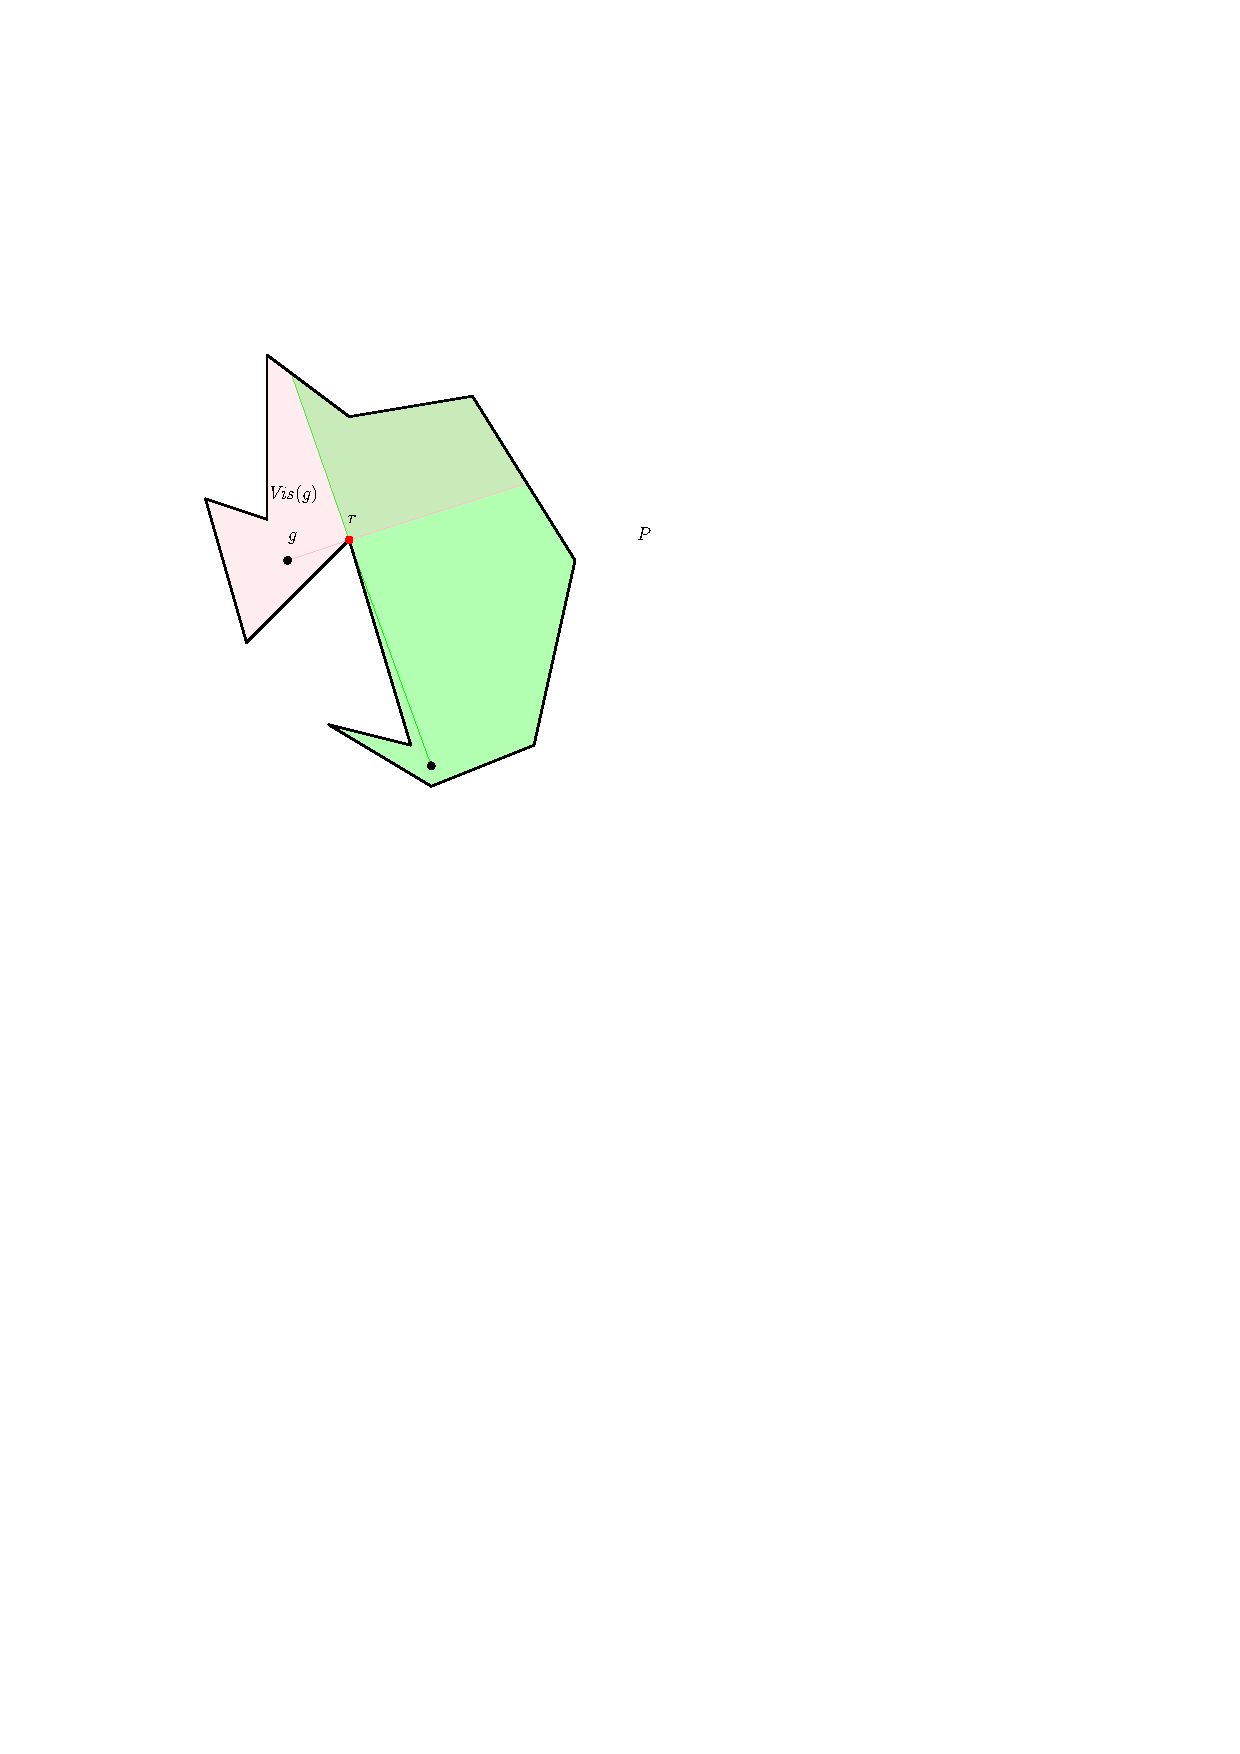
\includegraphics{theory/visp.pdf}
    \caption{Example of an Art Gallery Problem instance with polygon $P$ guarded by 2 guards. The visibility area $\mathit{Vis}(g)$ is emphasised in pink.}
    \label{fig:art}
\end{figure}

The Art Gallery Problem is $\exists \mathbb R$-complete \cite{abrahamsen2021art}, which means it is even harder to solve than NP-complete problems \cite{schaefer2009complexity}. For this reason, approximation algorithms have been extensively used to address it (\cite{DBLP:journals/corr/BonnetM16b}, \cite{GHOSH2010718}, \cite{DBLP:journals/corr/abs-2007-06920}). Nonetheless, to the best of our knowledge there is no related work on approaching the Art Gallery Problem using gradient descent. As such, we will approach the Art Gallery Problem from a new perspective using gradient descent.

\newpage
\subsection{Gradient Descent}

Gradient descent is an iterative optimisation algorithm for finding the minimum of a continuous differentiable function. The core idea of gradient descent is to repeatedly move in the opposite direction of the gradient of the function at the current point using a specific step size (learning rate). High learning rates result in approaching a local optimum faster, but risk overshooting it. Conversely, small learning rates are more precise, with the compromise of a longer computation and convergence time.
When there is no more change in the gradient, then an optimum has been reached. Gradient descent does not guarantee that the found optimum is global. For this reason, it can remain stuck in local optima.

Figure \ref{fig:gradient_descent} illustrates an intuitive example of applying gradient descent. The optimisation function takes the shape of a curve. Starting from an arbitrary point on the curve, the goal is to reach the minimum of the function (the bottom of the curve). This is done by computing the gradient (derivative) of the function at the current point. The gradient is displayed in red and tells that the largest increase in value for the function is going up the curve. Because we are interested in finding the minimum of the function, we have to move in the opposite direction of the gradient. So, we have to move down the curve with the given step size. Continuing from the new point on the curve, the process is repeated until the minimum is reached.
If we were interested in finding the maximum of the function, we would move in the same direction with the gradient.

\begin{figure}[h!]
    \centering
    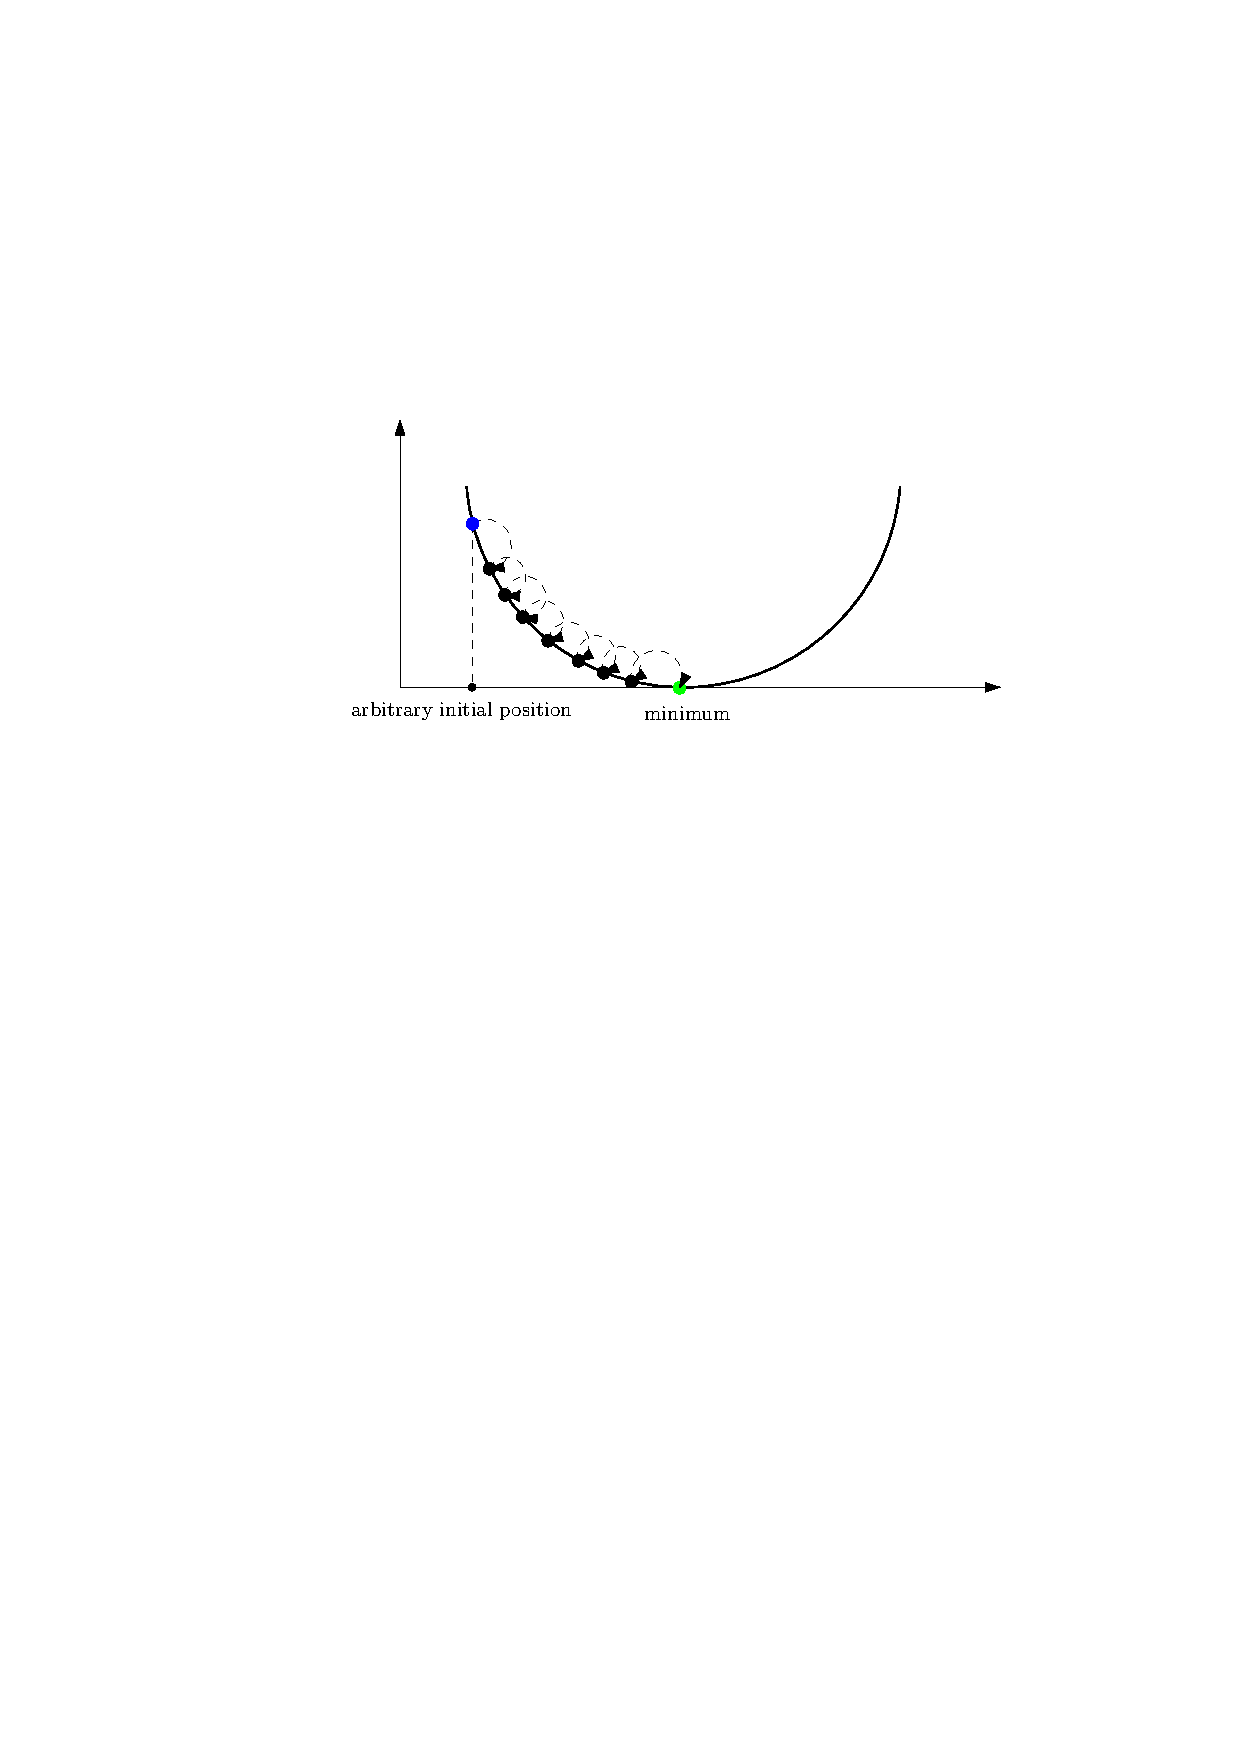
\includegraphics{gradient.pdf}
    \caption{Illustrative example of applying gradient descent.}
    \label{fig:gradient_descent}
\end{figure}

\subsection{Thesis Goal}
This thesis will thus be an optimisation algorithm engineering paper. The main goal is to create and implement an algorithm that uses gradient descent to approximate the solution to the Art Gallery Problem. The explored research question will be whether the Art Gallery Problem can be efficiently solved using gradient descent. Additional to gradient descent, the algorithm will deploy different heuristics to address various shortcomings and edge-cases.
% As such, we expect to be able to provide convergence guarantees for the algorithm. 
The algorithm will be implemented in C++ using the CGAL library \cite{cgal}.

This paper is organised as follows: Section \ref{sec:literature} offers an overview of existing work. Section \ref{sec:theory} explains how in theory gradient descent is used to solve the Art Gallery Problem and what heuristics we can make use of to improve the performance of our algorithm. Section \ref{sec:experiments} offers an overview of how well our algorithm performs in practice. Lastly, Section \ref{sec:problems} discusses issues this project has encountered.
% As such, preliminary research and its implementation is presented as preparation for the second phase of the thesis project. Section \ref{sec:literature} offers an existing literature overview. Next, Section \ref{sec:theory} describes the relevant theory in detail.
% As a preview, Section \ref{sec:experiments} shows some introductory algorithm implementations and their performance.
% Lastly, Section \ref{sec:thesis} presents the development plan for the second phase of the Master's Thesis project.

\section{Literature Summaries}
\label{sec:literature}
% Scientific back ground : What is the existing technology and literature that you will be studying/using in my research 

This section offers an overview of previous works addressing the Art Gallery Problem \cite{o1987art}. 
Working with the visibility region is a basic tool in computational geometry, specifically in the context of the Art Gallery Problem. The Art Gallery Problem is an $\exists \mathbb R$-complete problem \cite{abrahamsen2021art}. The problem class $\exists \mathbb R$ consists of instances that can be reduced in polynomial time to a decision problem of whether a system of polynomial equations with integer coefficients and any number of real variables has a solution. Since NP $\subseteq \exists \mathbb R$, the $\exists \mathbb R$ class is an at least as hard to solve complexity class. That is due to the fact that $\exists \mathbb R$-complete problems are not know to have solutions of polynomial space. 
% For this reason, it is crucial that the computation time of the visibility region is efficiently implemented. 

Building on the aforementioned concepts, this section will further inspect how visibility in polygons can be efficiently computed \cite{DBLP:journals/corr/BungiuHHHK14}, how it is not always possible to place guards at rational coordinates~\cite{abrahamsen2021art}, in addition to two improved polygon guarding algorithms \cite{maleki2022implementation}, \cite{DBLP:journals/corr/abs-2007-06920}.
% Some general notions that will appear in the papers are introduced below.

% Visibility in simple planar polygons can be defined as: given a polygon $P \subset \mathbb R^2$, a point (guard) $p \in P$ \textit{sees} a point $q \in P$ if the line segment $\overline{pq} \subseteq P$. Thus, the points that are visible from $p$ form the visibility polygon (region) $\mathit{Vis}(p)$.

% A guard set $S$ is defined as a set of points in a given polygon $P$ such that every point in $P$ is seen by some point in $S$. $\forall x, y \in P$, $x$ sees $y$ if the line segment $\overline{xy} \in P$. 

\subsection{Efficient Computation of Visibility Polygons}
Bungiu, Hemmer, Hershberger, Huang and Kr\"oller  \cite{DBLP:journals/corr/BungiuHHHK14} introduce the implementations and their experimental evaluations for two existing algorithms (\cite{joe1987corrections}, \cite{asano1985efficient}) and a newly developed one for computing visibility in polygons. These implementations are available in the CGAL library \cite{cgal}, starting with version 4.5.


Therefore, Bungiu et al. present three algorithms and their practical performance.

\subsubsection{Algorithm of Joe and Simpson}
The algorithm of Joe and Simpson \cite{joe1987corrections} runs in $O(n)$ time and space. 

Let $v_i$, for $i = {1, 2, ..., n}$, be the boundary vertices of the polygon $P$. Let $g$ be a guard in $P$, and let $s$ be a stack data structure. The stack $s$ will be used to keep track of the vertices determining $\mathit{Vis}(g)$. 

The algorithm begins by scanning the boundaries of $P$. The scanning is done through shooting rays $\vec{pv_i}$, for $i = {1, 2, ..., n}$ in this order. The endpoints $v_i$ and $v_{i + 1}$ of each ray form a boundary edge $\overline{v_iv_{i + 1}}$. In this way, the processing of $v_i$ and $v_{i + 1}$ is done by checking whether the points are in $\mathit{Vis}(g)$. This means that the position of every $v_{i + 1}$ with respect to the ray $\vec{pv_i}$ is checked. If $v_{i + 1}$ is found in front of the ray $\vec{pv_i}$ (if $v_{i + 1}$ is seen from $g$), then both $v_i$ and $v_{i + 1}$ are added to the processing stack $s$. For every newly pushed vertex on $s$, the algorithm checks whether the segment $\overline{v_iv_{i + 1}}$ obscures any of the previously added vertices. If that is the case, then the endpoints of the obscured line segment are declared obsolete and deleted. The polygon comprised of the vertices from $s$ forms at the end the visibility polygon $\mathit{Vis}(g)$.

% TODO: this might need better explanation? not sure if edge cases are needed
Figure \ref{fig:joe} displays an example run of the Algorithm of Joe and Simpson \cite{joe1987corrections} for polygon $P$ and guard $g$. First, the ray from $g$ is shot through vertex $v_1$, and $v_1$ is added to $s$. Then, the ray from $g$ is shot through $v_2$. Since ray $\vec{pv_2}$ takes a right turn from $\vec{pv_1}$, this means that $v_2$ is still in the visibility region of $g$. For this reason, $v_2$ is also added to $s$. The ray passing through $v_2$ also intersects the boundary of $P$ in a point $v_2'$. To account for the fact that $g$ can see ``behind'' $v_2$ and is still inside $P$, the boundary vertex $v_2'$ is hence added to $s$. Next, the ray $\vec{pv_3}$ takes a left turn from $v_2$, which means that $v_3$ is not seen from $g$. 

\newpage
\begin{figure}[h!]
	\centering
	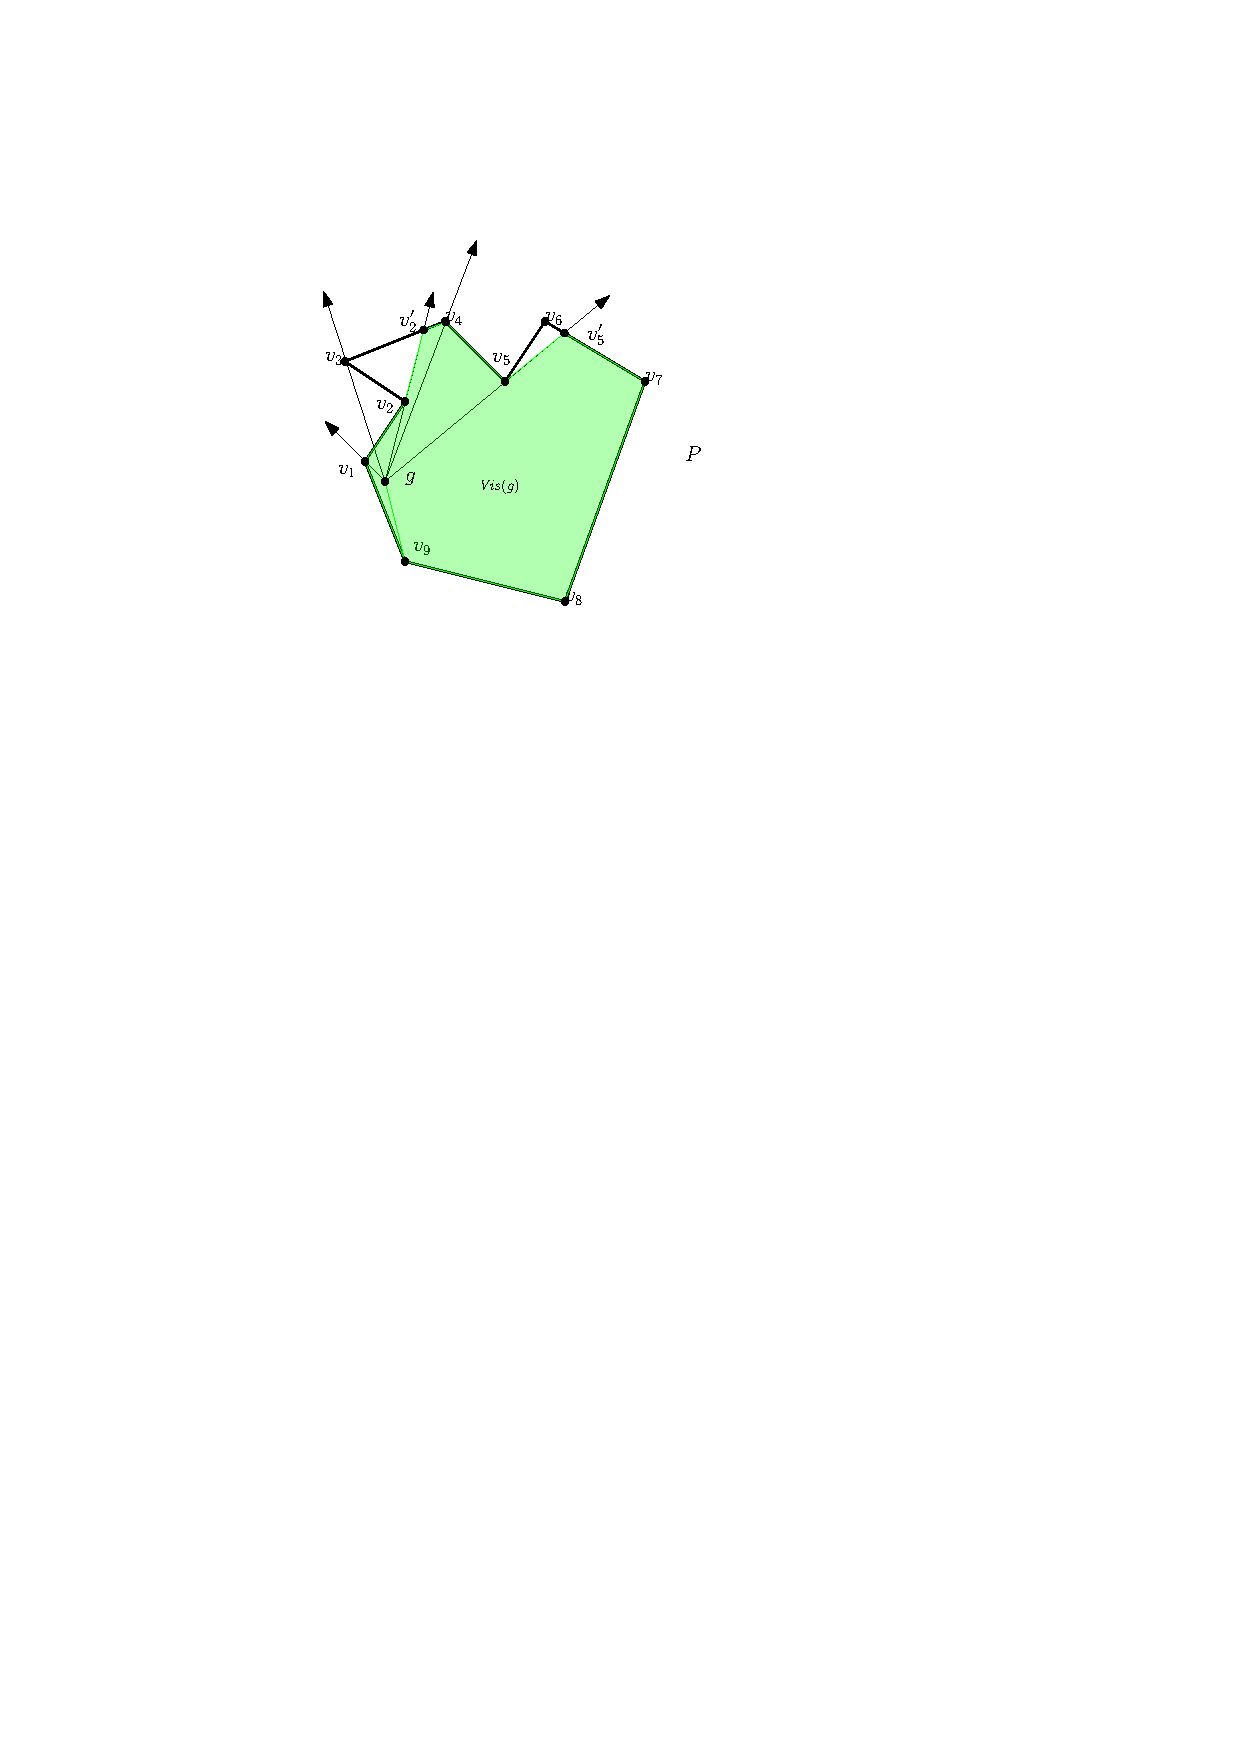
\includegraphics{literature/joe_simpson_eg.pdf}
	\caption{An example run of the algorithm of Joe and Simpson \cite{joe1987corrections} for polygon $P$ guarded by $g$ and boundary vertices $v_i$, for $i = \{1, 2, ..., n\}$.}
	\label{fig:joe}
\end{figure}

\noindent
Similarly, $v_4$ and $v_5$ are added to $s$. However, because ray $\vec{pv_6}$ takes a left turn from $\vec{pv_5}$, segment $\overline{v_5v_6}$ obscures $\overline{v_4v_5}$. So, $v_4$ and $v_5$ are removed from $s$. Ray $\vec{pv_6}$ then intersects the boundary of $P$ in $v_6'$. At the end, $\mathit{Vis}(g) = \{v_1, v_2, v_2', v_6, v_6', v_7, v_8, v_9, v_{10}\}$, as shown on the boundary of the green area. 



% boundaries of t	he simple polygon $P$, and adds its boundary points $v_i, \forall i = \overline{1, n}$, with $n$ the number of vertices in $P$, to a stack $s$. For each processed edge $\overline{v_iv_{i + 1}}$, its endpoints $v_i$ and $v_{i + 1}$ are checked whether they are in the visibility region of the viewpoint $g$. If they are, $v_i$ and $v_{i + 1}$ are added to~$s$. Otherwise, they are skipped. At every moment, the algorithm checks whether $\overline{v_iv_{i + 1}}$ obscures a previously added line segment. If that is the case, then the endpoints of the obscured line segment are declared obsolete and deleted. 

% The implementation of the algorithm handles the previously discussed cases for an arrangement $P$, while also accounting for the case in which the polygon winds more than 360$^\circ$ using a winding counter.
% - **Algorithm of Joe and Simpson** $O(n)$ time and space
	% - performs a sequential scan of the boundary of $P$ and uses a stack $s$ of boundary points $s_0, s_1, ..., s_ as summarised in the following subsections.der to deal with cases in which the polygon winds more than 360*, a winding counter is used during this edge processing
% he points that are visible from $q$ form the visibility region $\mathcal V(q)$ (polygon)
% \newpage
\subsubsection{Algorithm of Asano}
The algorithm of Asano \cite{asano1985efficient} runs in $O(n \log n)$ time and $O(n)$ space. It uses a plane sweep approach with event line $L$. 

Let $P$ be a polygon determined by vertices $\{a_1, a_2, a_3, b_1, b_2, b_3, b_4\}$. $P$ may have holes. Suppose we want to guard it by point $g$. The algorithm of Asano \cite{asano1985efficient} begins by efficiently sorting all the vertices of $P$ based on their polar angles with respect to the guard $g$. Figure \ref{fig:asano_1} displays an example run of the algorithm. The points will be treated in the order of $a_2, a_1, a_3, b_4, b_3, b_2, b_1$ with respect to $g$ and their angular comparisons $$\measuredangle a_2Op < \measuredangle a_1Op < \measuredangle a_3Op < \measuredangle b_4Op < \measuredangle b_3Op < \measuredangle b_2Op < \measuredangle b_1Op,$$ where $O = (0, 0)$.


Then, the event line $L$ starts sweeping around $g$ as shown in Subfigures \ref{fig:asano1} - \ref{fig:asano7}. Every line segment that $L$ intersects is stored in a balanced binary tree $T$ in the order of their intersection angle. As $T$ is updated, a new vertex of $\mathit{Vis}(g)$ is stored each time the segment closest to $g$ in $T$ changes. It is important to mention that the intersection between $L$ and the line segments is not explicit, but is instead determined by comparisons between the endpoints' coordinates. For instance, in Figure \ref{fig:asano_1}, the endpoint $b_2$ of line segment $\overline{b_2a_2}$ is the first one $L$ intersects. Point $b_2$ is thus added to $T$. Then, $L$ continues sweeping and adds $b_1, a_2$ and $a_1$ to $T$. Although $\overline{b_2a_2}$ and $\overline{b_1a_1}$ represent line segments $s_2$ and $s_1$, respectively, the intersection of $L$ with them is not explicitly computed, but is determined based solely on the positions of their endpoints: $s_1$ is farther away from $g$ because $q, a_2$ and $b_2$ are on the same side of $s_2$.

\newpage
\begin{figure}[h!]
	\centering
	\begin{subfigure}{0.45\textwidth}
		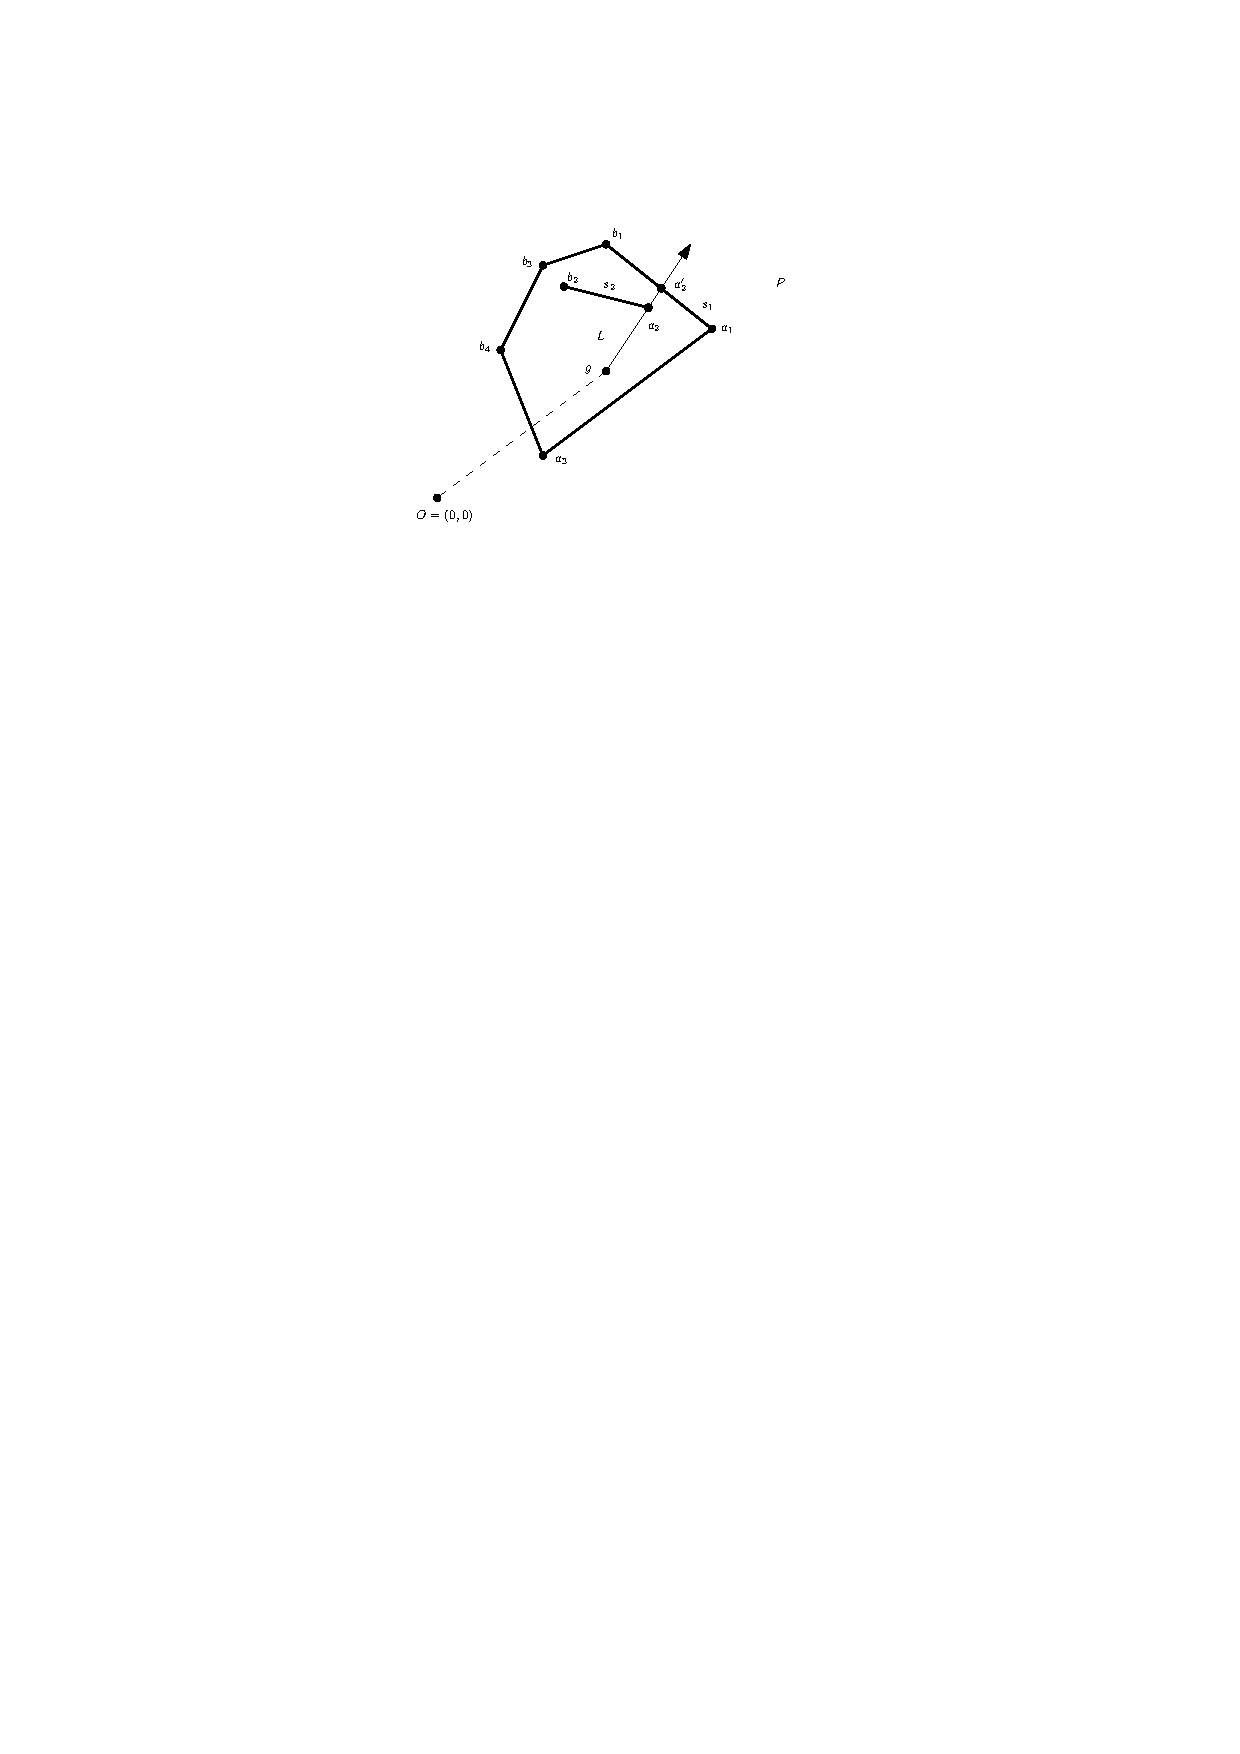
\includegraphics{literature/asano7.pdf}
		\caption{$a_2$ is added to the empty $\mathit{Vis}(g)$ such \\ that $\mathit{Vis}(g) = \{a_2\}$.}
		\label{fig:asano1}
	\end{subfigure}
	\hfill
	\begin{subfigure}{0.45\textwidth}
		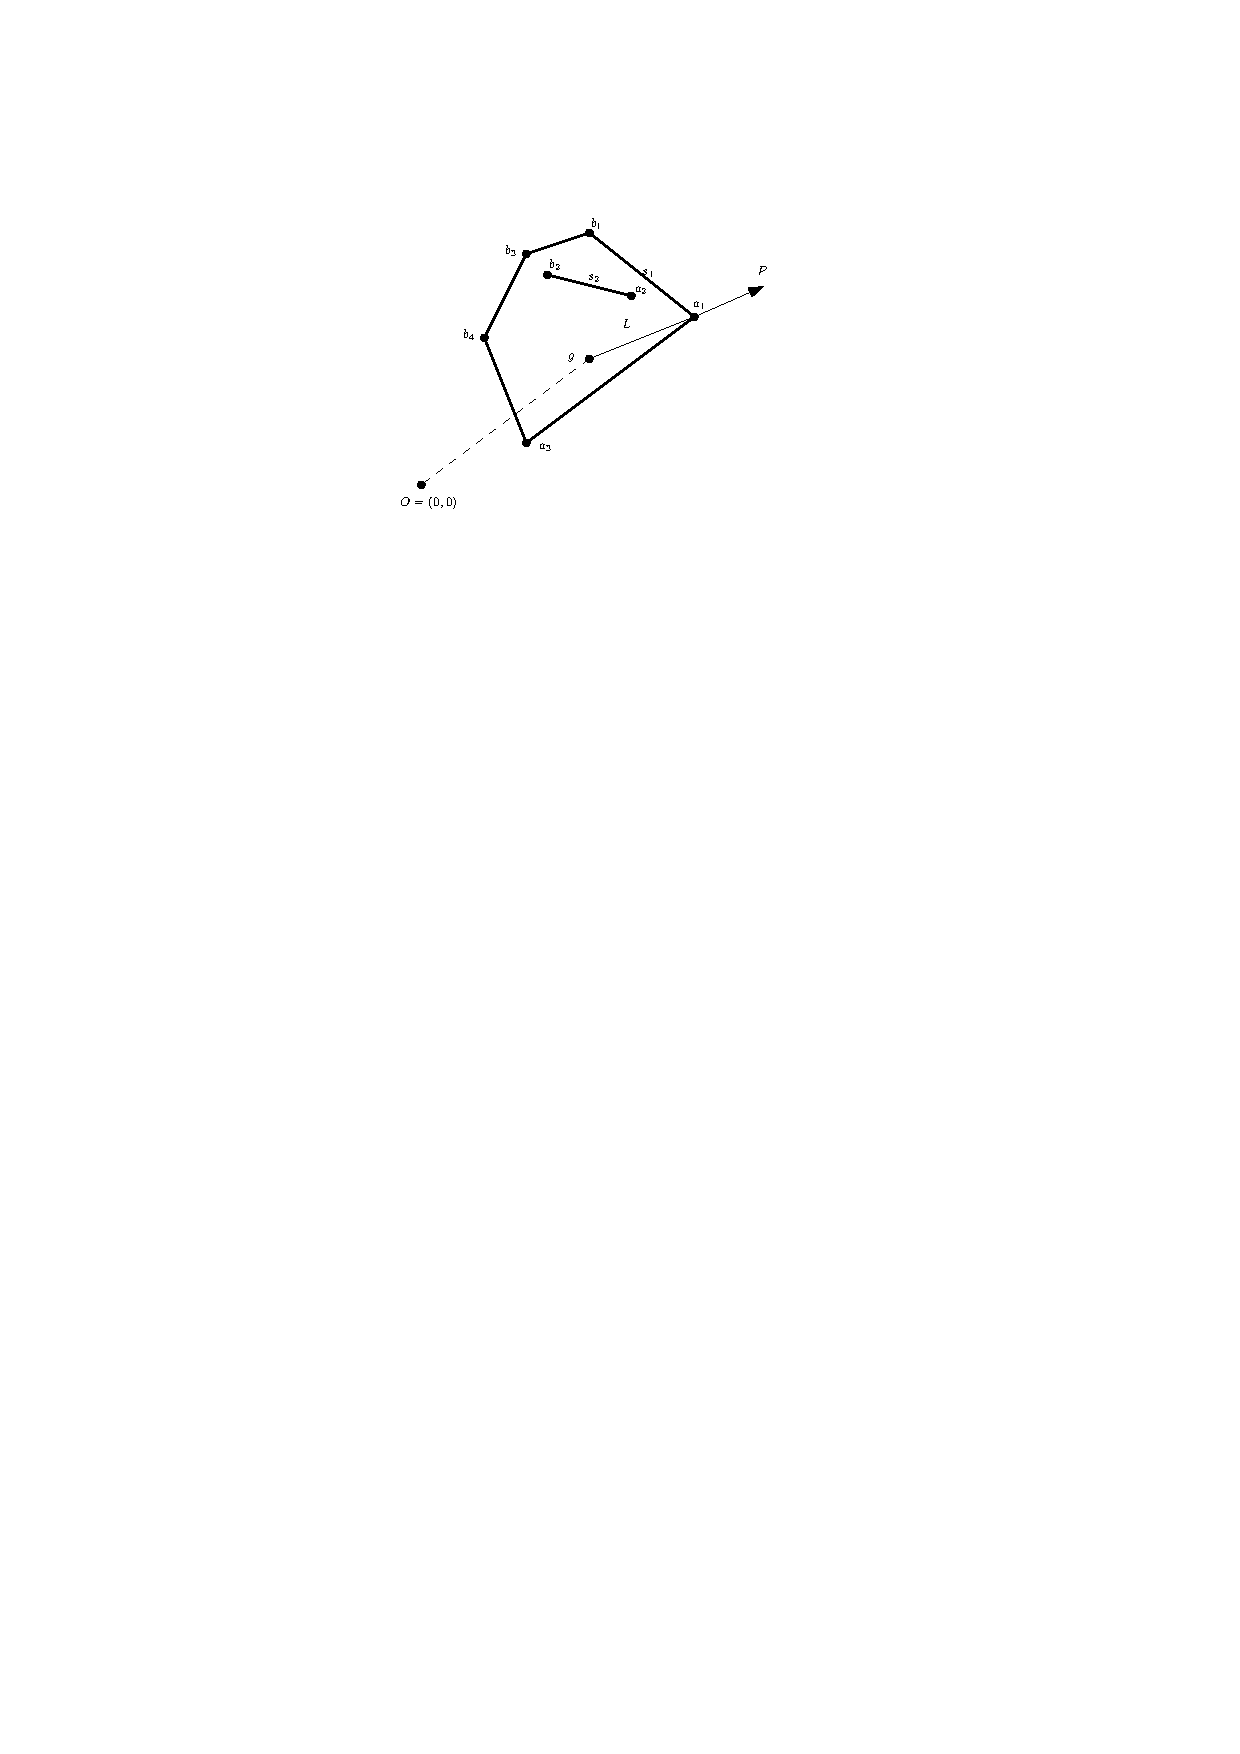
\includegraphics{literature/asano1.pdf}
		\caption{$a_1$ is added to $\mathit{Vis}(g)$ such that \\ $\mathit{Vis}(g) = \{a_1, a_2\}$, and line segment $\overline{b_1a_1}$ is added to the empty binary tree $T = \{\overline{b_1a_1}\}$.}
	\end{subfigure}
	\begin{subfigure}{0.45\textwidth}
		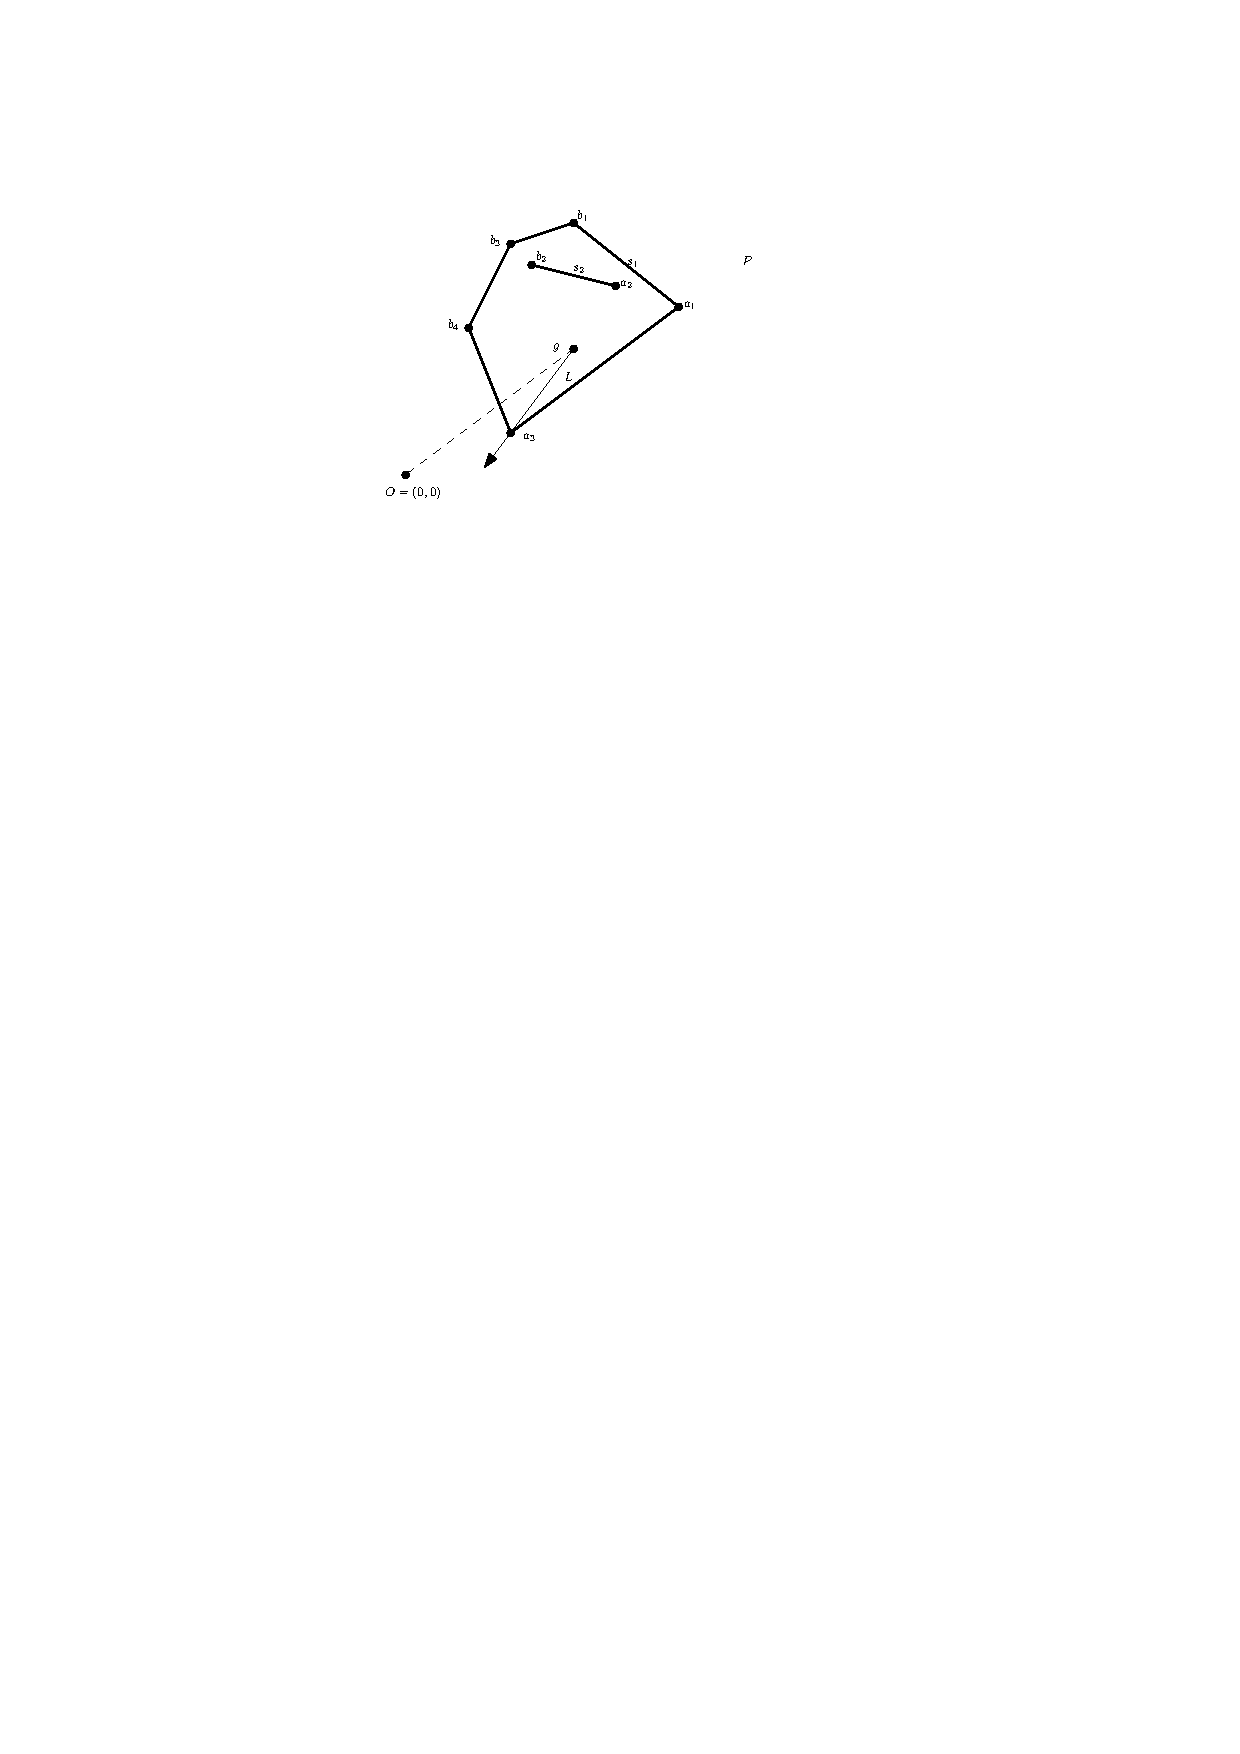
\includegraphics{literature/asano2.pdf}
		\caption{$a_3$ is added to $\mathit{Vis}(g)$ such \\ that $\mathit{Vis}(g)~=~\{a_1, a_2, a_3\}$,  and line \\ segment $\overline{a_1a_3}$ is added to $T$ such that \\ $T = \{\overline{b_1a_1}, \overline{a_1a_3}\}$.}
	\end{subfigure}
	\hfill
	\begin{subfigure}{0.45\textwidth}
		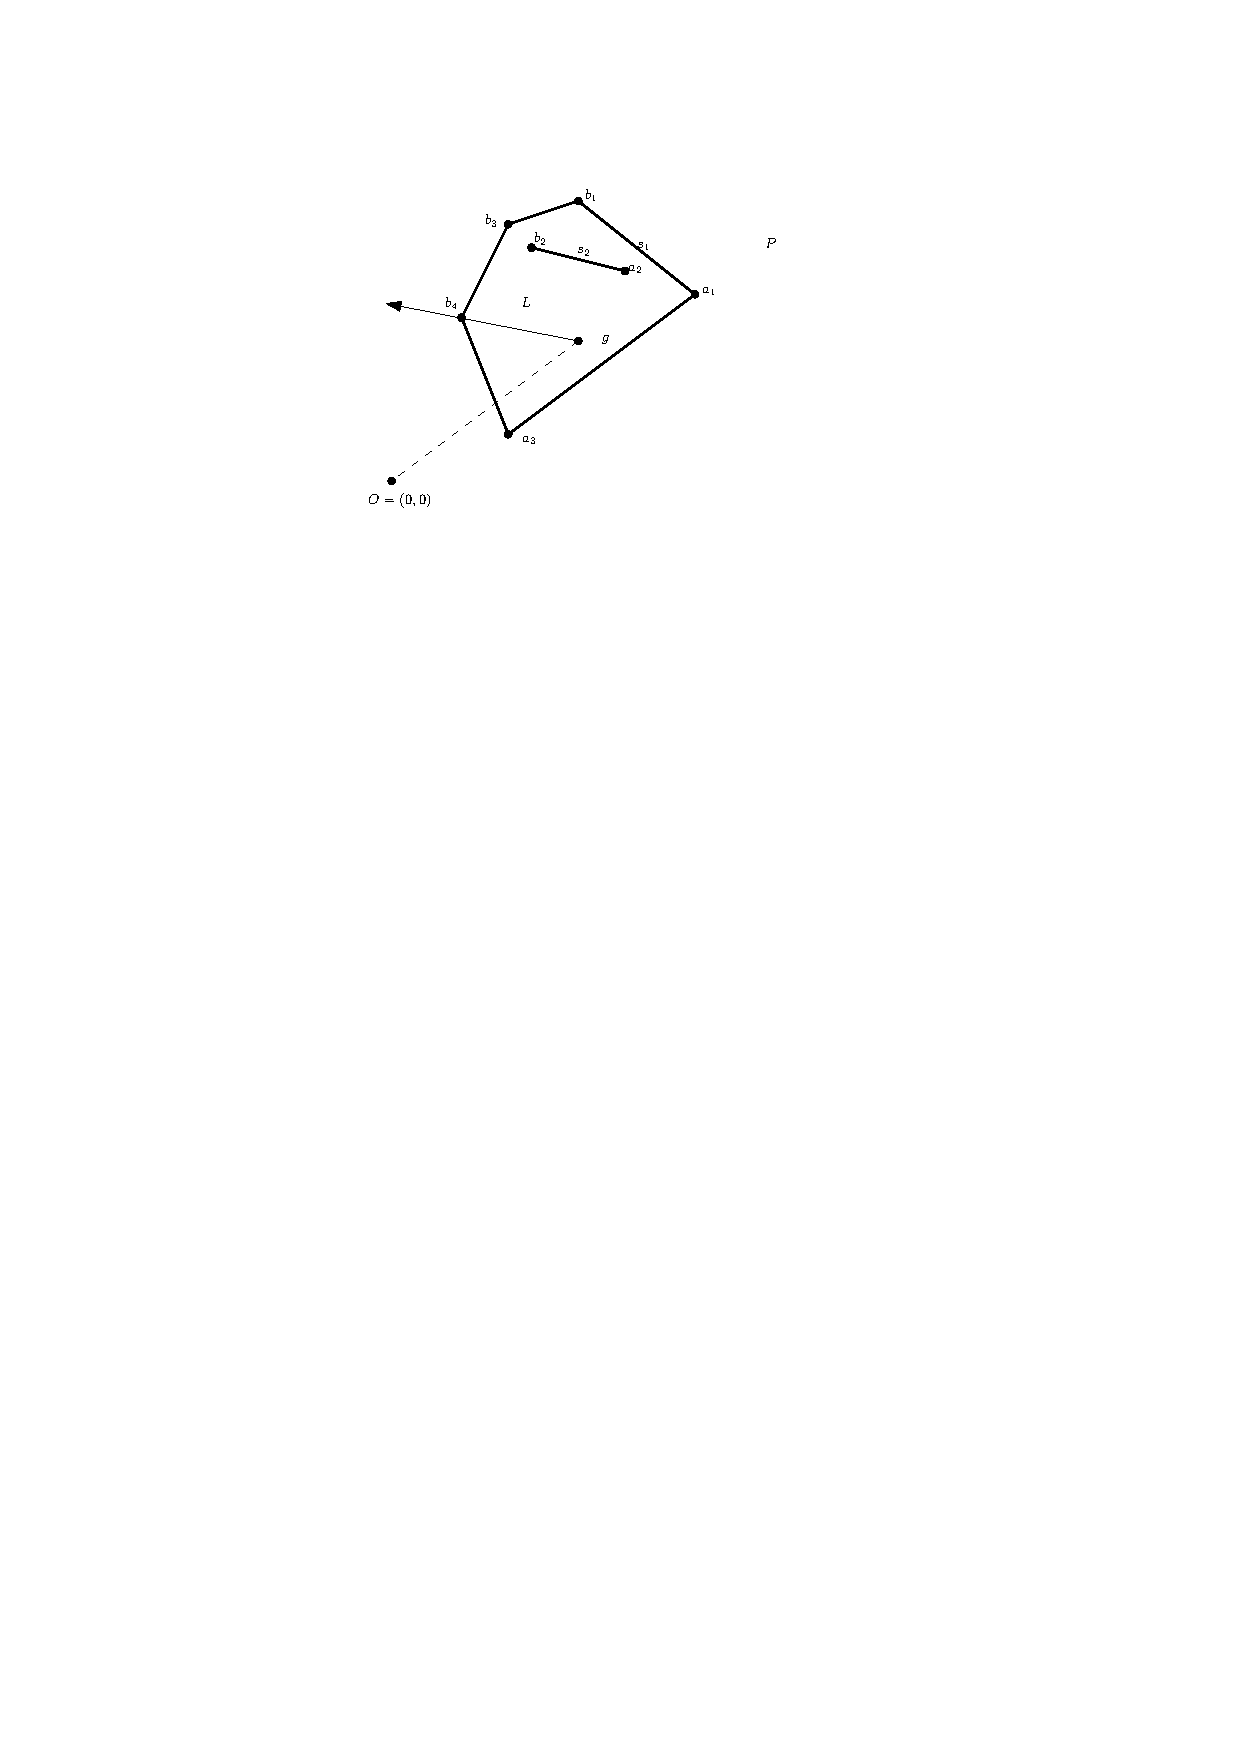
\includegraphics{literature/asano3.pdf}
		\caption{$b_4$ is added to $\mathit{Vis}(g)$ such \\ that $\mathit{Vis}(g)=\{a_1, a_2, a_3, b_4\}$, and line \\ segment $\overline{a_3b_4}$ is added to $T$ such that \\ $T = \{\overline{b_1a_1}, \overline{a_1a_3}, \overline{a_3b_4}\}$.}
	\end{subfigure}
	\begin{subfigure}{0.45\textwidth}
		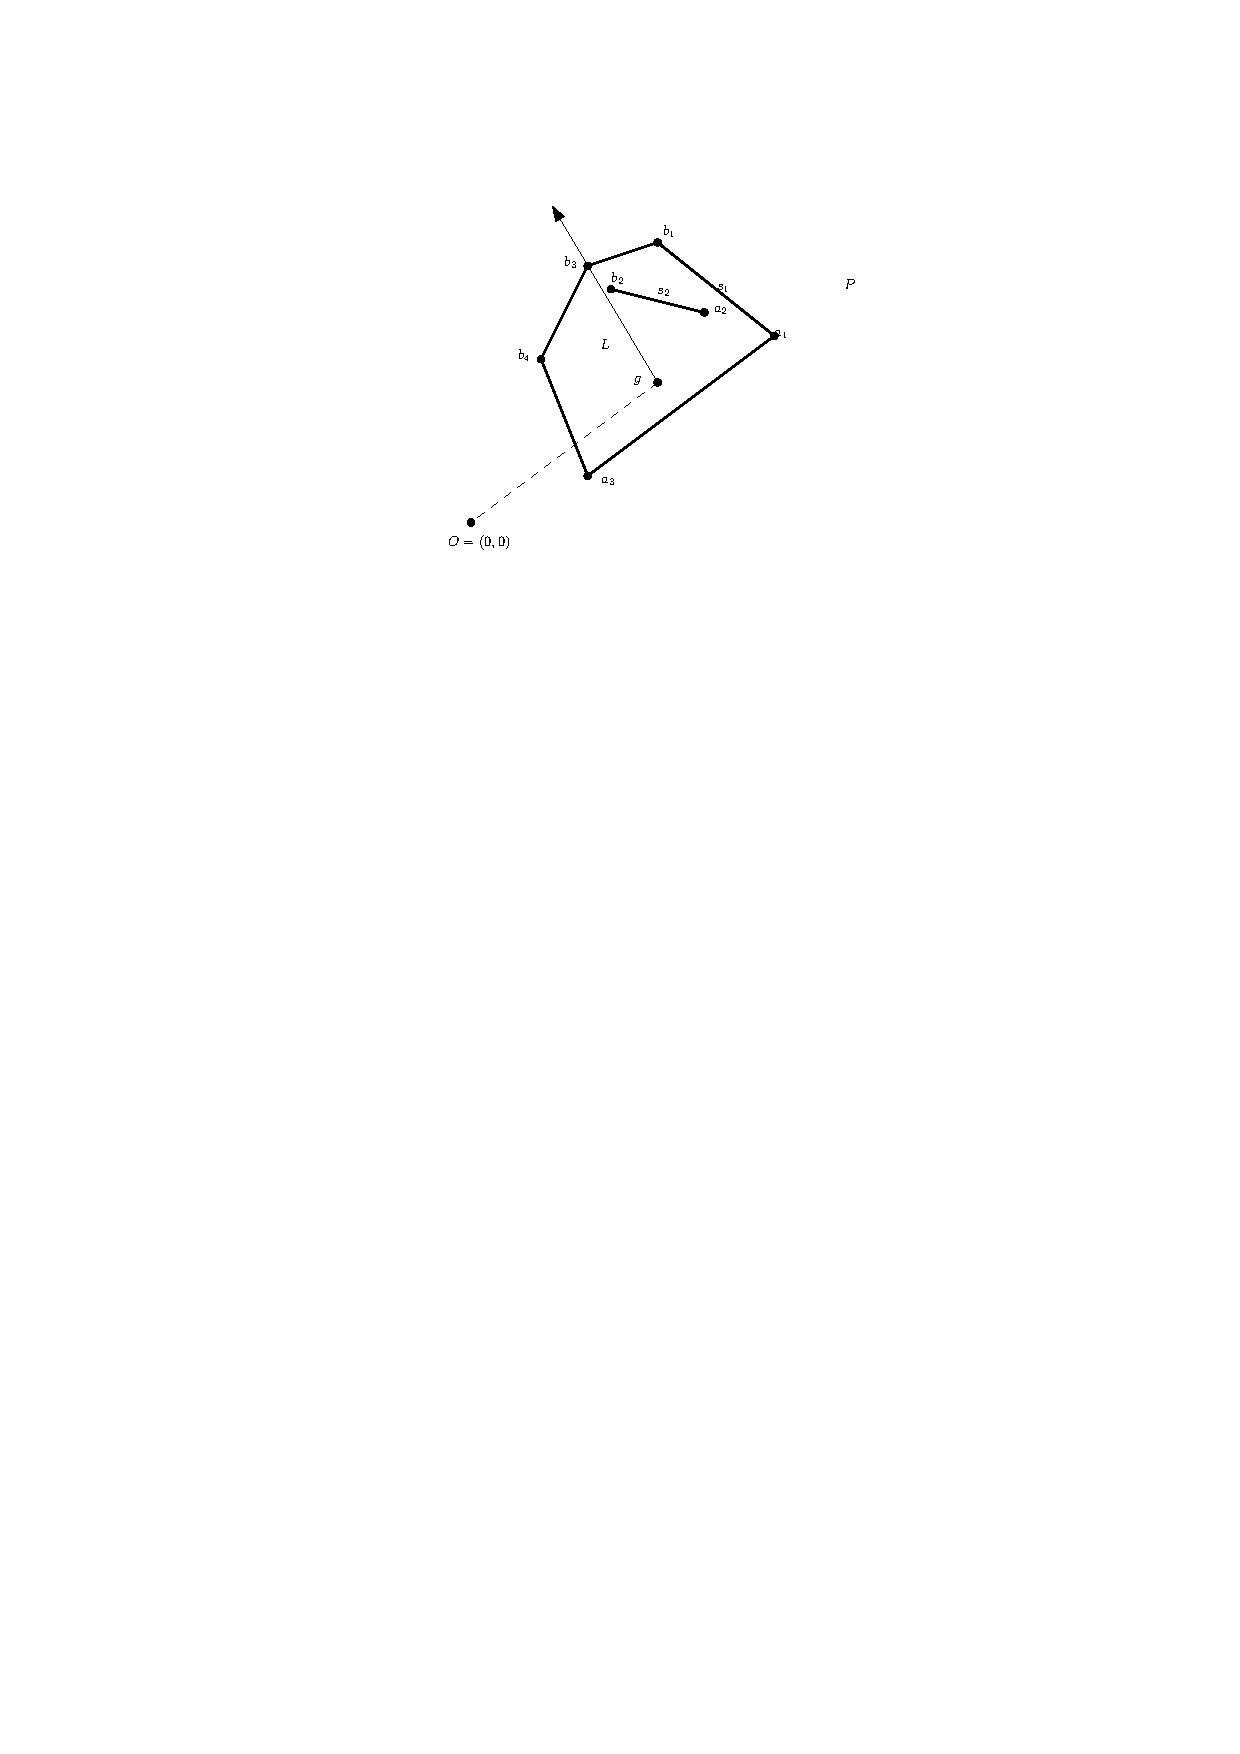
\includegraphics{literature/asano4.pdf}
		\caption{$b_3$ is added to $\mathit{Vis}(g)$ \\ such that $\mathit{Vis}(g)=\{a_1, a_2, a_3, b_4, b_3\}$, \\ and line segment $\overline{b_4b_3}$ is added to $T$ \\ such that $T = \{\overline{b_1a_1}, \overline{a_1a_3}, \overline{a_3b_4}, \overline{b_4b_3}\}$.}
	\end{subfigure}
	\hfill
	\begin{subfigure}{0.45\textwidth}
		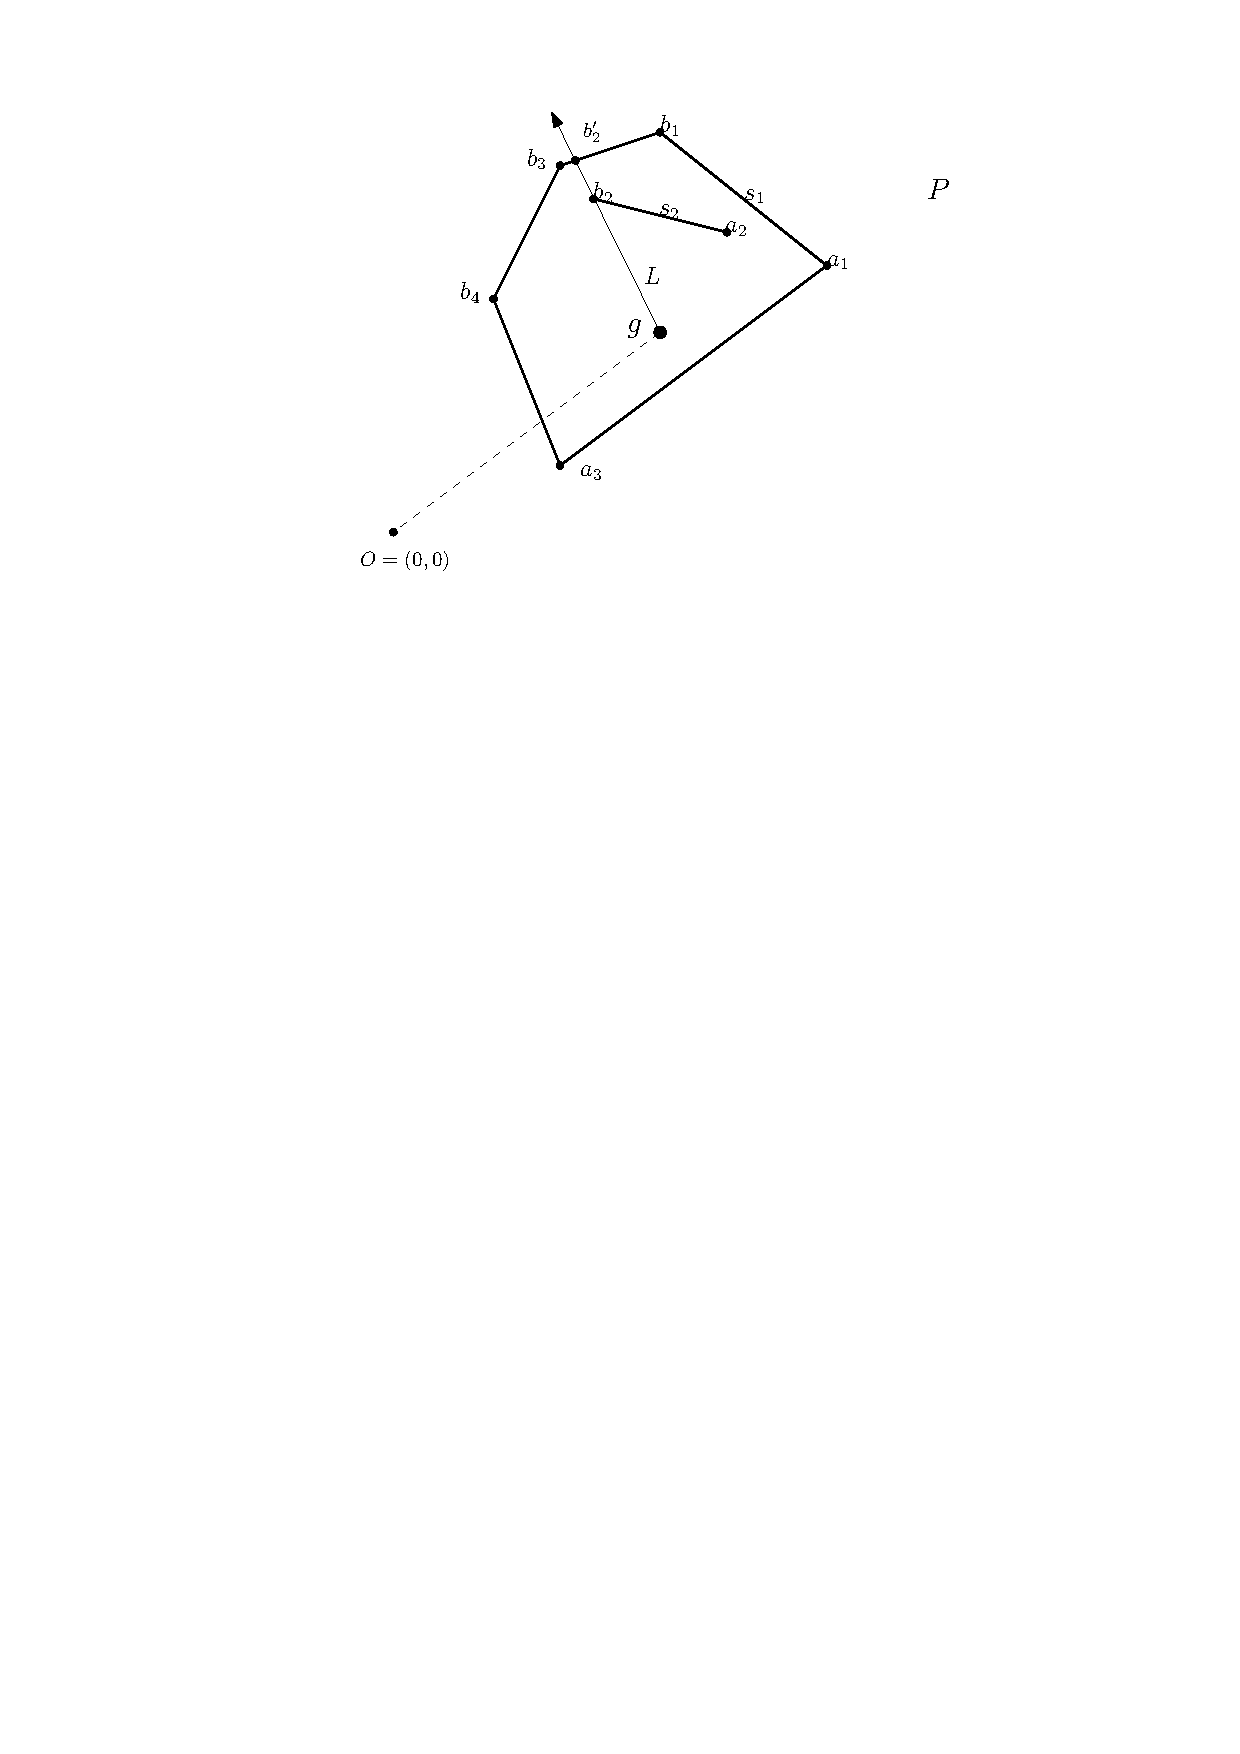
\includegraphics{literature/asano5.pdf}
		\caption{$b_2$ is added to $\mathit{Vis}(g)$ such that \\ $\mathit{Vis}(g) = \{a_1, a_2, a_3, b_3, b_4, b_2\}$, and line segment $\overline{b_2a_2}$ is added to $T$ such that \\ $T = \{\overline{b_1a_1}, \overline{a_1a_3}, \overline{a_3b_4}, \overline{b_4b_3}, \overline{b_2a_2}\}$.}
	\end{subfigure}
	\caption{Example run of the Algorithm of Asano \cite{asano1985efficient} on polygon $P$ and guard $g$. The vertices of $P$ are added to the binary tree $T$ in the order of their angle between $g$ and the origin $O = (0, 0)$. The result of the algorithm is visibility region $\mathit{Vis}(g) = \{a_1, a_2, a_3, b_3, b_4, b_2\}$.}
	\label{fig:asano_1}
\end{figure}
\begin{figure}[h!]
	\ContinuedFloat
	\centering

	\begin{subfigure}{\textwidth}
		\centering
		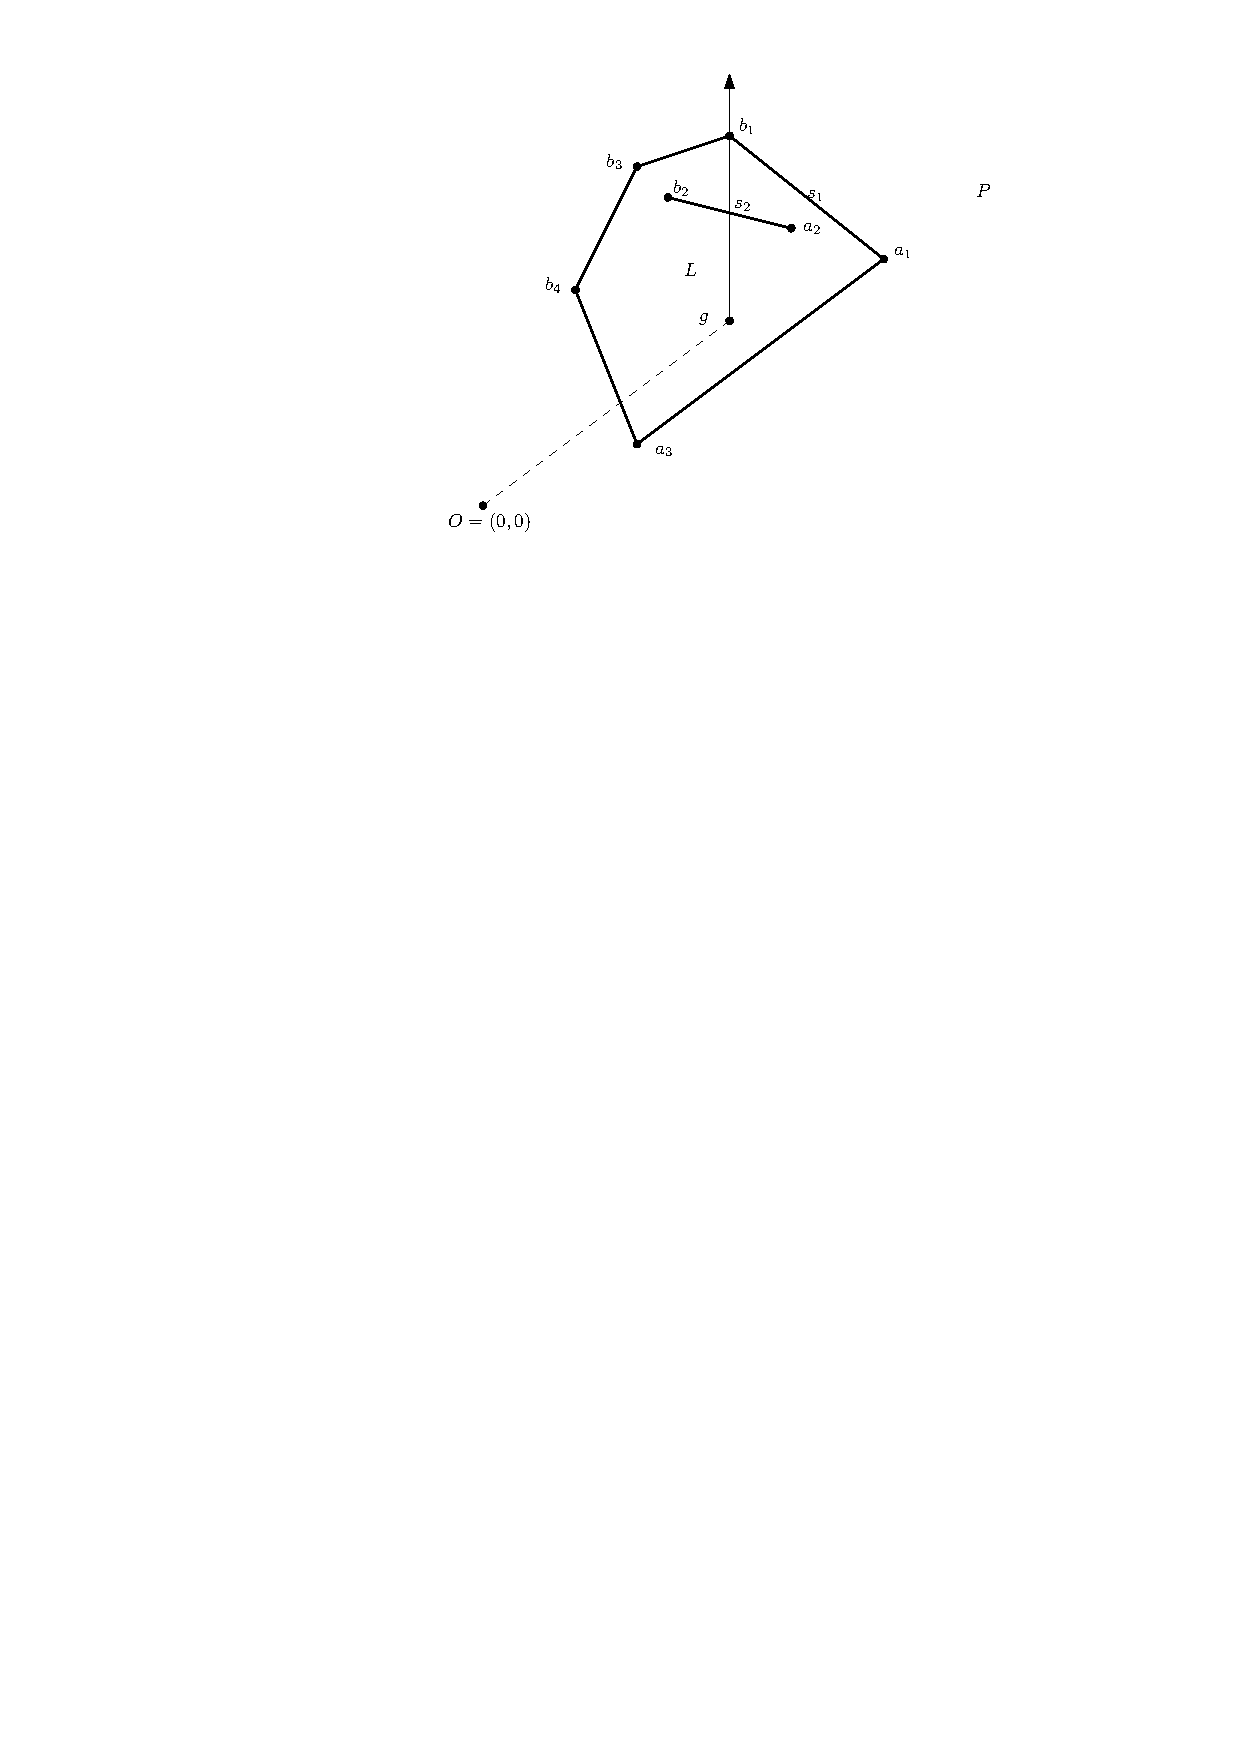
\includegraphics{literature/asano6.pdf}
		\caption{$b_1$ is not added to $\mathit{Vis}(g)$ because it is obstructed by the line segment $\overline{b_2a_2}$ which is already in $T$. For the same reason, line segments $\overline{b_3b_1}$ and $\overline{b_1a_1}$ are also not added in $T$.}
		\label{fig:asano7}
	\end{subfigure}
	\caption{Example run of the Algorithm of Asano \cite{asano1985efficient} on polygon $P$ and guard $g$. The vertices of $P$ are added to the binary tree $T$ in the order of their angle between $g$ and the origin $O = (0, 0)$. The result of the algorithm is visibility region $\mathit{Vis}(g) = \{a_1, a_2, a_3, b_3, b_4, b_2\}$.}
	\label{fig:asano_2}
\end{figure}



% \begin{figure}[h!]
% 	\centering
% 	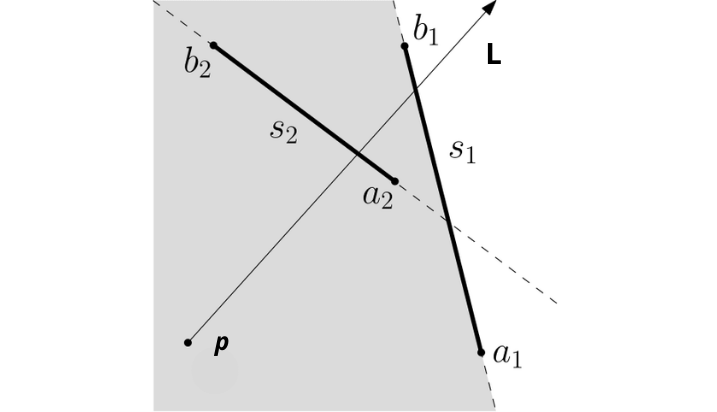
\includegraphics[width = 0.5\textwidth]{compare_segments.png}
% 	\caption{The Algorithm of Asano \cite{asano1985efficient} Visual Example \cite{DBLP:journals/corr/BungiuHHHK14}.}
% 	\label{fig:asano}
% \end{figure}
	% - as the sweep proceeds, $T$ is updated and a neq vertex of $V(q)$ is generated each time the smallest element (segment closest to $q$) in $T$ changes
	% - important to have efficient comparison ops (e.g.: *add pic*)
% \newpage 
\subsubsection{New Algorithm: Triangular Expansion}
The algorithm introduced by Bungiu et al. \cite{DBLP:journals/corr/BungiuHHHK14} is named Triangular Expansion and runs in $\Omega(n^2)$ time and $O(n)$ space. It begins by triangulating $P$ in $O(n \log n)$ time if $P$ has holes, and $O(n)$ otherwise. The implementation runtime is constrained by CGAL, which makes use of the Delaunay triangulation algorithm \cite{delaunay1934sphere} with $O(n^2)$ time for the worst case, but with better performance in practice. 

Taken from \cite{DBLP:journals/corr/BungiuHHHK14} and annotated to suit the explanations in these summaries, Figure \ref{fig:triangular} depicts an example run of the algorithm on a polygon with holes $P$. Starting from the viewpoint $g$, the triangle containing $g$ is located by performing a simple walk. Trivially, $g$ sees the entire triangle it is contained in. The algorithm continues by recursively expanding the view of $g$ from one triangle into the next, until there are no more triangles to expand into. The view of $g$ becomes restricted by the reflex vertices $l$ and $r$ of the third triangle entered by the recursive step. Since $l$ and $r$ are reflex vertices, the view past them is further restricted until the boundaries $l'$ and $r'$ of $P$, respectively,  are reached. Line segments $\overline{ll'}$ and $\overline{rr'}$ are added to $\mathit{Vis}(g)$ in their angular order around $g$. At the end, $\mathit{Vis}(g)$ will contain the segments delimiting the visibility polygon of $g$.

\begin{figure}[h!]
	\centering
	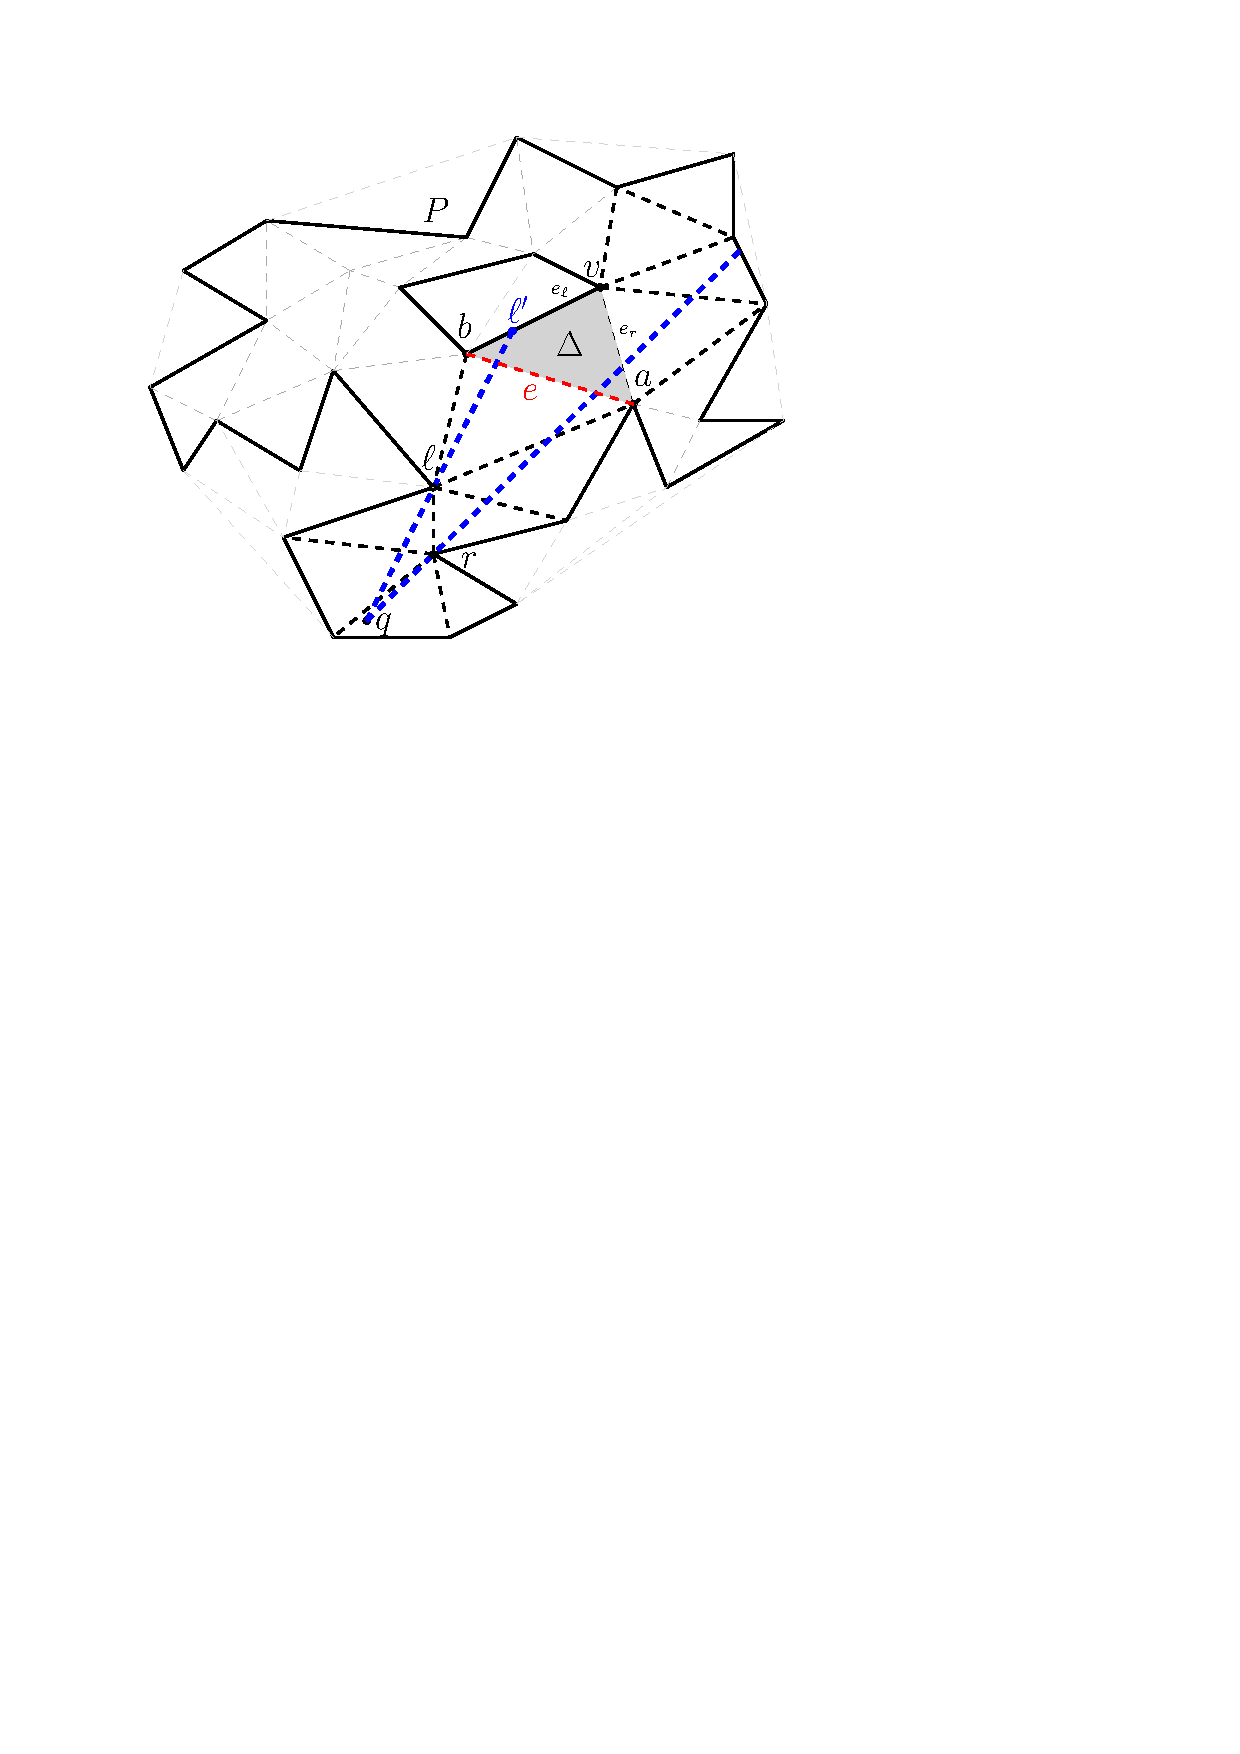
\includegraphics{literature/triangular_expansion.pdf}
	\caption{The Triangular Expansion Algorithm Example - recursion entering triangle $\Delta$ through edge~$e$~\cite{DBLP:journals/corr/BungiuHHHK14}.}
	\label{fig:triangular}
\end{figure}
% - **triangular expansion** - $O(n^2)$
	% - preprocessing: triangulation ($O(n)$ for simple polygons, $O(n\log n$) for polygons with holes; Delaunay ($O(n^2)$) used)
	% - given $q$, locate the triangle containing $q$ by a simple walk ($q$ sees the entire triangle)
	% - recursive procedure that expands the view of $q$ through that edge into the next triangle. Initially, the view is restricted by the 2 endpoints of the edge, and then further as recursion continues: *add pic* for triangle $\Delta$, the view of $q$ is restricted by the 2 reflex vertices $l$ and $r$ with $a \leq r < l \leq b$ w.r.t. angular order around $q$. $v$ is a new vertex and its position w.r.t. $l$ and $r$ is computed with 2 orientation tests *add pic*: $e_l$ is a boundary edge and we can report edge $\overline{ll'}$ and $\overline{l'v}$ as part of the visibility region of $q$; $e_r$ is not a boundary edge => the recursion continues with $v$ being the vertex that now restricts the left side of the view
	% - the recursion may split into 2 calls if $e_l$ and $e_r$ are both not part of the boundary. As there are $n$ vertices, this can happen $O(n)$ times => worst-case $O(n^2)$; however a true split into two visibility cones that may reach the same triangle independently can only happen at a hole of $P$, thus at worst the runtime is $O(nh)$, where $h$ = number of holes (linear time of simple polygons) (e.g.: worst-case *add pic*)
	% - triangulation has linear size, at most $O(n)$ recursive calls on the stack => $O(n)$ space

\subsubsection{Experiments}
Bungiu et al. do not report on benchmarks with query points on edges in the interior polygon. This is because they claim that their implementations perform similarly to other already implemented algorithms. Instead, they use two real-world scenarios (a simple polygon of Norway with 20981 vertices, and a cathedral polygon with 1209 vertices) and a worst-case polygon for the Triangular Expansion algorithm.

In terms of results on the real-world polygons, the Triangular Expansion algorithm has a 2-factor improved performance when compared to Asano's algorithm \cite{asano1985efficient}, and performs ``one order of magnitude'' faster than Joe and Simpson's algorithm \cite{joe1987corrections}. For the worst-case scenario, Asano's algorithm \cite{asano1985efficient} outperforms the Triangular Expansion algorithm with increasing input complexity.

Thus, despite the Triangular Expansion algorithm being outperformed in the worst-case scenario, Bungiu et al. add efficient implementations for  3 different  polygon visibility algorithms in the CGAL library. The choice of algorithms when using the library can be adapted based on the input polygons. 
% - experiments - no reports on similar benchmarks with query points on edges and in the interior polygon; for the input graphs used, the triangular expansion is 2-factor faster than Asano, and one order of magnitude faster than Joe and Simpson; with increasing input complexity, Asano does become faster
\subsection{Irrational Guards Are Sometimes Needed}
Abrahamsen, Adamaszek, and Miltzow \cite{abrahamsen2021art} study the placement of the guards in the context of the Art Gallery Problem \cite{o1987art}. Namely, it focusses on and confirms that there are polygons with integer coordinates that require guards placed at points with irrational coordinates. Generalising, Abrahamsen et al. show that $\forall n \in \mathbb N$, there is a family of simple monotone polygons that can either be guarded by $3n$ guards with irrational coordinates, or requires at least $4n$ guards with rational coordinates. The result is also extended to a rectilinear polygon that can be guarded by 9 guards with irrational coordinates, or requires at least 10 guards with rational coordinates. The family of simple monotone polygons that can be guarded by $3n$ guards with irrational coordinates, as well as the rectilinear polygon that can be guarded by 9 guards with irrational coordinates are also discussed.


% Before the time of the writing, there was no combinatorial algorithm for finding an optimal solution for The Art Gallery Problem \cite{o1987art}, nor for its decidability version on whether a set $S$ of given size $k$ exists. As such, it was not known whether the problem is in NP.

First, we will address the question regarding whether polygons given by integer coordinates require guard positions with irrational coordinates in any optimal solution by introducing a crafted monotone polygon $P$. A polygon is monotone if there exists a line $l$ such that every line orthogonal to $l$ intersects its boundary at most twice. Polygon $P$ is depicted in Figure \ref{fig:p} and is constructed using a rectangle, six triangular pockets (in green), three rectangular pockets (in blue) and four quadrilaterial pockets (in red) are added. The intuition behind the polygon will be explained in the upcoming subsections. The figure is accredited to Abraham et al. \cite{1057165}.

\begin{figure}[h!]
    \centering
    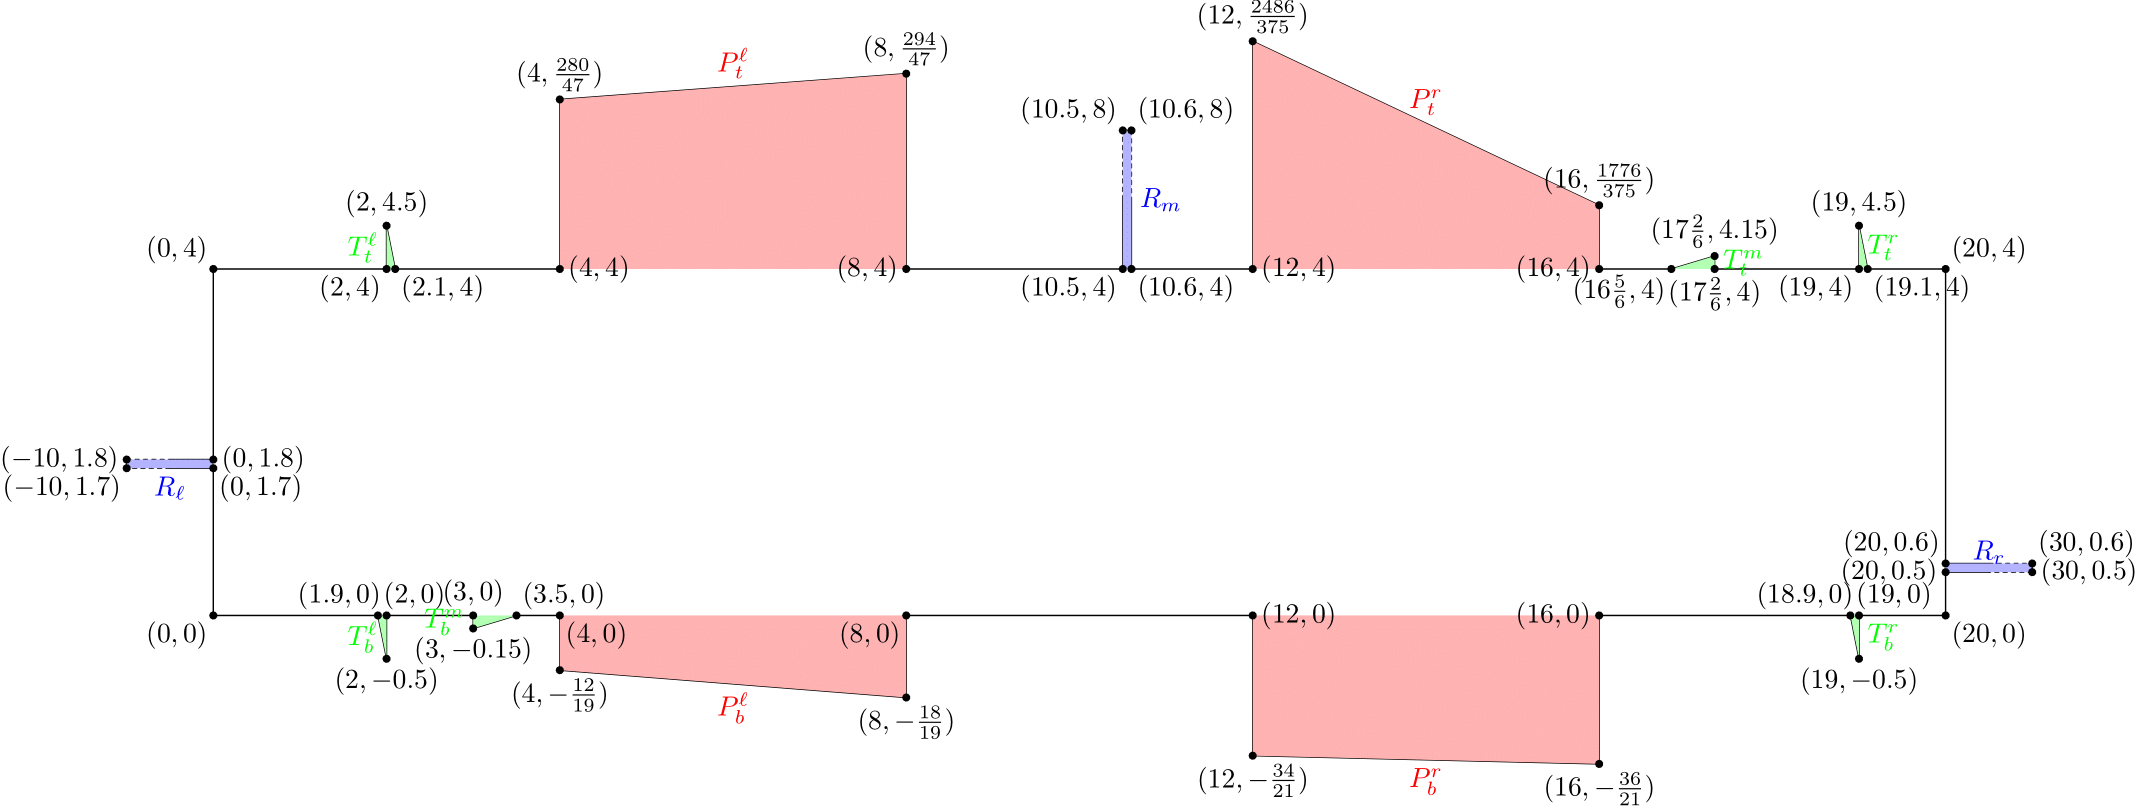
\includegraphics[width=\textwidth]{literature/fig-12-1.png}
    \caption{The polygon $P$ developed by Abraham et al \cite{1057165} to emphasise the need for irrational guards sometimes.}
    \label{fig:p}
\end{figure}

\newpage
\subsubsection{Intuition for Triangular Pockets}
The six triangular pockets are created in order to force a guard on a line segment, as depicted in Figure \ref{fig:tb}. The figure is taken from \cite{abrahamsen2021art}. As such, they are grouped into three pairs: top pockets are paired with bottom pockets corresponding to their position in $P$. For every pair (leftmost, middle, rightmost) of triangular pockets, there is a corresponding line $l_\ell, l_m, l_r$, respectively, that joins the peaks of each triangular pocket in a pair. A guard can see both the peaks $t, b$ of the pockets only if it is placed on the line segment $\overline{tb}$ (Figure \ref{fig:forcing_line}). Hence, one guard is needed per pair, resulting in 3 guards in total.

\begin{figure}[h!]
    \centering
    % 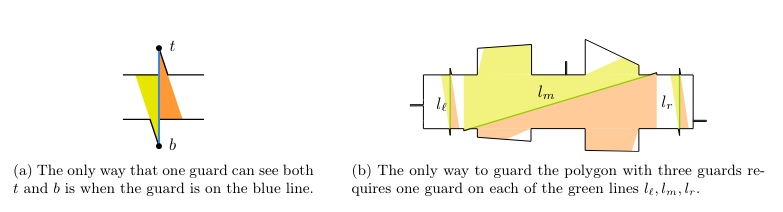
\includegraphics[width=\textwidth]{Screenshot from 2022-02-02 09-57-44.png}
    \begin{subfigure}{0.3\textwidth}
        \centering
        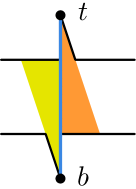
\includegraphics[width=0.45\textwidth]{literature/ForcingLine-1.png}
        \caption{The only way that one guard can see both $t$ and $b$ is when the guard is on the blue line.}
        \label{fig:forcing_line}
    \end{subfigure}
    \hfill
    \begin{subfigure}{0.65\textwidth}
        \centering
        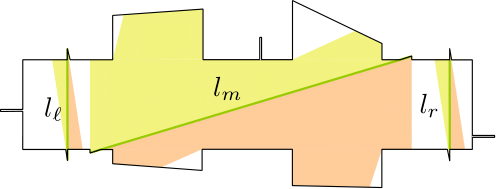
\includegraphics[width=0.6\textwidth]{literature/DisjointTriangleRegions2-1.png}
        \caption{The only way to guard the polygon with three guards requires one guard on each of the green lines $l_\ell, l_m, l_r$.}
        \label{fig:disjoint_triangle}
    \end{subfigure}
    \caption{Forcing guards to lie on specific line segments \cite{1057165}.}
    \label{fig:tb}
\end{figure}

\subsubsection{Intuition for Quadrilaterial Pockets}
The four quadrilateral pockets are created in order to force a guard in a region bounded by a curve. Figure \ref{fig:quadrilateral_pockets} was taken and adapted from \cite{1057165}, and depicts the visualisation for this case. 
Consider some position of $g_{\ell}$ on $l_{\ell}$. As $g_{\ell}$ moves up on $l_{\ell}$, the point $p^{\ell}_t$ slides towards the right on segment $e^{\ell}_t$, and point $p^{\ell}_b$ slides to the left on segment $e^{\ell}_b$. In this way, the lines $p^{\ell}_tb$ and $p^{\ell}_bd$, where $b, d$ are reflex vertices, intersect and form the curve $c_{\ell}$. Considering thus the fixed position of a guard $g_m$ either on the left or on the right of the curve $c_\ell$, there exists a position of guard $g_{\ell}$ on $l_{\ell}$ such that edge $e_t^{\ell}$ and line $p_b^{\ell}g_m$ are seen by $g_\ell$. Then, only if $g_m$ is on the left or on $c_\ell$ can it see the remaining parts of the pockets that are not seen by $g_\ell$ (edge $e_b^{\ell}$, line $p_t^{\ell}g_{\ell}$). Analogously, in order for the right side of $P$ and the right pair of quadrilateral pockets to be seen by both guards $g_m$ and $g_r$, $g_m$ has to be on the curve $c_r$ or on its right. Since $g_m$ has to also satisfy its position on $l_m$, its only feasible position is as the intersection point between $c_\ell, c_r$ and $l_m$. 

\begin{figure}[h!]
    \centering
    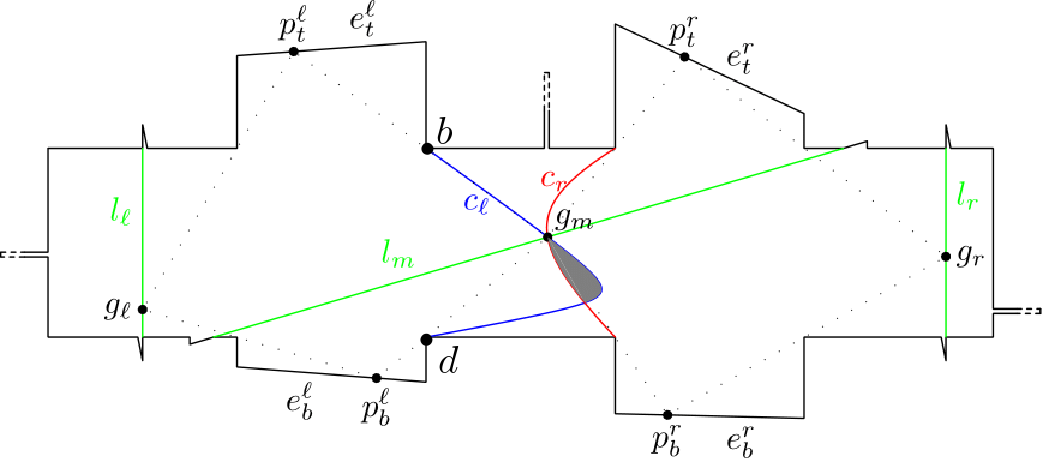
\includegraphics[width=0.7\textwidth]{literature/fig-6-1.png}
    \caption{Restricting a guard to a region bounded by a curve \cite{1057165}.}
    \label{fig:quadrilateral_pockets}
\end{figure}

\subsubsection{Intuition for Rectangular Pockets}
The three rectangular pockets are created in order to force a guard to a single irrational point. Further building onto the previously discussed instance from Figure \ref{fig:quadrilateral_pockets}, the three rectangular pockets on the laterals and top of $P$ are added.  They allow for additional constraints for the positions of the guards $g_\ell, g_m, g_r$. Based on the curve equations of $c_\ell$ and $c_r$, we can thus calculate the irrational position of $g_m = (3.5 + 5\sqrt 2, 1.5\sqrt 2)$. Subsequently, we can fix the positions of $g_\ell$ and $g_r$ on lines $l_\ell$ and $l_r$.

\subsubsection{Monotone Polygon Construction}
The polygon $P$ in question  was found through experimentation in GeoGebra (\url{https://www.geogebra.org/}). The triangular and rectangular pockets were fixed. Finding then the position of the rectangular pockets required the existence of a rational line that contained the irrational coordinates of guard $g_m$ from Figure \ref{fig:quadrilateral_pockets}. The irrational coordinates of the two other guards $g_\ell, g_r$ were chosen such that they would be able to see the rest of the polygon that is unseen by $g_m$. The rectangular pockets were added based on their coordinates.

In this way, by placing each guard placed on the lines $l_\ell, l_m, l_r$ at unique irrational positions, respectively, dependencies between guard positions were created. The resulting guard set becomes thus $S = \{g_\ell, g_m, g_r\}$.  Given the unique and irrational positions of the guards, the only method for seeing the whole polygon $P$ using guards with rational positions would be to use at least 4. This statement can also be generalised such that a family of polygons $(\mathcal{P}_n)_{n \in \mathbb{Z}_+}, \forall n$ can be guarded by $3n$ guards with irrational coordinates, or requires $4n$ guards with rational coordinates. The coordinates determining the polygons are hence polynomial in $n$.

\subsubsection{Rectilinear Polygon Construction}
Similarly, a rectilinear polygon $P_R$ can be created given integer coordinates. Polygon $P_R$ would require guards with irrational coordinates in any optimal solution. It can be guarded by 9 guards if guards can be placed at points with irrational coordinates. Otherwise, the smallest optimal guard set $S$ with rational coordinates would be required to have size 10.

Polygon $P_R$ can be constructed by extending $P$ with the 6 non-rectiliniar gray parts ($Q_1, Q_2, Q_3, Q_4, T_1, T_2$) in Figure \ref{fig:rectilinear}, such that each of them requires at least 1 guard in the interior. The figure was taken from \cite{1057165}. When placing 6 guards in the gray parts, the white areas of $P_R$ remain unseen. As such, 3 guards must still be similarly placed at the 3 irrational points on lines $l_\ell, l_m, l_r$ as in the case of $P$, in order to guard the rest of $P_R$.

\begin{figure}[h!]
    \centering
    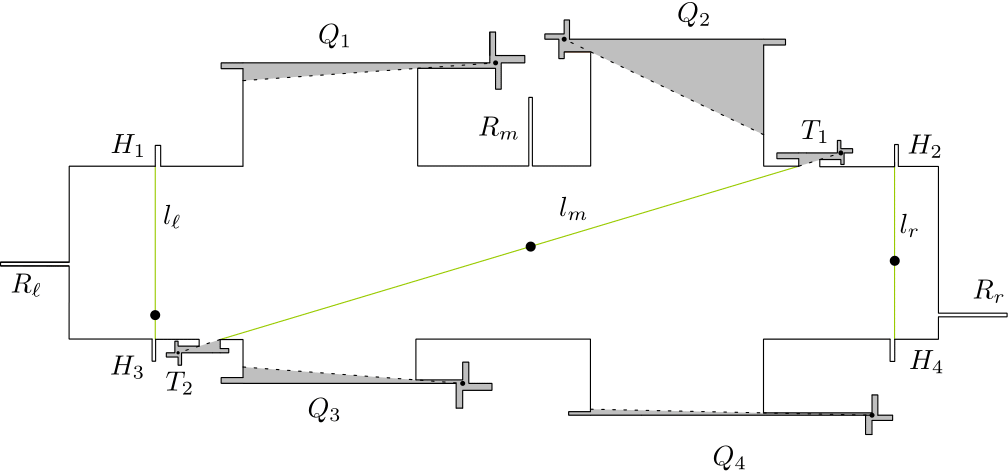
\includegraphics[width=0.7\textwidth]{literature/RectilinearPolygonComplete4-1.png}
    \caption{Rectilinear Polygon $P_R$ \cite{1057165}.}
    \label{fig:rectilinear}
\end{figure}
% a guard at position $x$ sees a point $y$ if the line segment $xy$ is fully contained in the polygon $\mathcal{P}$
% - a _guard set_ $S$ is a set of points in $\mathcal{P}$ s.t. every point in $\mathcal{P}$ is seen by some point in $S$ - find a minimum cardinality guard set for a simple polygon $\mathcal{P}$ on $n$ vertices
% - research less focussed on the classical problem, but more on its variations
% - no combinatorial algorithm for finding an optimal solution, or even for deciding whether a guard set of a given size $k$ exists, only real algebraic geometry powerful tools - not known if in NP
% - given polygons by integer coordinates, do they require guard positions with irrational coordinates in any optimal solution?
	% => yes, by constructing a _monotone_ polygon ($\exists$ line $l$ s.t. every line orthogonal to $l$ intersects $P$ at most twice) with integer coordinates that can be guarded by three guards only when we allow to place the guards at points with irrational coordinates; otherwise, 4 guards are needed
			% - *place pic*
			% - **forcing a guard on a line segment** by creating 3 triangular pockets *pic* that can enforce 3 guards on 3 line segments within $P$ - a guard can see both $t$ and $b$ if it is on the blue line segment $tb$, which is the intersection of 2 regions => $k$ pairs of triangular pockets and no 2 regions corresponding to different pairs of pockets intersecting => in order to guard the polygon with $k$ guards, there must be one guard on the line segment corresponding to each pair
			% - **restricting a guard to a region bounded by a curve** - consider a fixed position of $g_2$ on or to the right of the segment $bd$. $\exists$ a position of $g_1$ on $l$ s.t. the entire polygon is seen by $g_1$ and $g_2$ iff. $g_2$ lies on or to the left of the curve $\mathcal C$ *insert pic*
			% - **restricting a guard to a single (irrational) point** - *insert pic* $g_m$ and $g_l$ can guard together the 2 left pockets, and at the same time $g_m$ and $g_r$ can guard together the two right pockets => $g_m$ can only be in the irrational point $p = (3.5 + 5\sqrt 2, 1.5\sqrt 2)$
			% - **searching for the polygon** - we need to force $g_m$ to be on a line $l_m$ containing $p$, but we can only force $g_m$ to be on a rational line => we require the existence of a rational line $l_m$ that contains $p$ - there can be at most one rational line containing the irrational point $p$, as any 2 rational lines intersect in a rational point => reverse-engineer the polygon, after having chosen the positions of the guards of the form $(r_1 + r_2\sqrt 2, r_3 + r_4\sqrt 2), r_1, r_2, r_3, r_4 \in \mathbb Q$ ; rectangle with pockets added
	% - consider any set $S$ for $P$ consisting of at most 3 guards: then $|S| = 3$ and $\exists$ 1 guard on each of the lines $l_l, l_m, l_r$
	% - consider any guard set $S$ for $P$ consisting of 3 guards; then 1 of the guards has an $x$-coord in $[10.5, 10.6]$. For the remaining 2 guards, $g_l$ has a $y$-coord in $i_1 = [0.5, 0.6]$ and the $g_r$ in $i_2 = [1.7, 1.8]$
	% - **dependencies between guard positions**
		% - the guards $g_l$ and $g_m$ together see all of $e_t^l$ and $e_b^l$ and the guards $g_m$ and $g_r$ together can see all of $e_t^r$ and $e_b^r$ *add pic*
	% - **computing the unique solution**
		% - the max $x$-coord of $g_m$ s.t. $g_l$ and $g_m$ can together see $e_t^l$ and $e_b^l$ is $x = 3.5 + 5\sqrt 2$. The corresponding position of $g_l$ is $(2, 2 - \sqrt 2)$
		% - the min $x$-coord of $g_m$ s.t. $g_r$ and $g_m$ can see both $e_t^r$ and $e_b^r$ is $x = 3.5 + 5\sqrt 2$. The corresponding position of $g_r$ is $(19, 1 + \frac{\sqrt 2}{2})$  
	% - $\forall n$, there is a family of polygons $(\mathcal{P}_n)_{n \in \mathbb{Z}_+}$ which can be guarded by $3n$ guards with irrational coordinates, but need $4n$ guards to be rational; the coordinates of the points defining the polygons $P_n$ are polynomial in $n$
	% - there is a rectilinear polygon $P_R$ given by integer coordinates that require guards with irrational coordinates in any optimal solution - $P_R$ can be guarded by 9 guards if we allow placing guards at points with irrational coordinates; an optimal guard set of $P_R$ with guards at points with rational coordinates has size 10
		% - start with $P$ - extend the non-rectilinear parts by "equivalent" rectilinear parts (gray) s.t. each of them requires at least  1 guard in the interior; if the interior of each pocket contains only 1 guard, then these guards must be placed at specific positions, making the area not seen by these 6 additional guards (white) => the remaining 3 guards must be placed at 3 irrational points (*place pic*)
% - _terrain guarding problem_ - $x$-monotone polygonal curve $c$ is given, the region $R$ above $c$ has to be guarded, and the guards are restricted to lie on $c$ - discretisation available in $O(n^3)$ time -> no irrational numbers phenomenon, and the decision version of the terrain guarding problem is in NP
\newpage
\subsection[Implementation of Guarding Algorithms]{Implementation of Polygon Guarding Algorithms for Art Gallery Problems}
Maleki and Mohades \cite{maleki2022implementation} introduce their implementations for two existing approximation algorithms (\cite{GHOSH2010718}, \cite{bhattacharya2016approximability}) for computing visibility in simple polygons. Additionally, they develop their own visibility algorithm. They lastly  evaluate experimentally their implementations for the three algorithms in the context of the Art Gallery Problem \cite{o1987art}.

To begin with, we will introduce some terminology used throughout this summary. The algorithms distinguish in their implementation between vertex guards and point guards in  a polygon $P$. Vertex guards can be placed only on the vertices of $P$. Point guards can be placed without restriction inside $P$. Lastly, the algorithms are tested on weak visibility polygons. A polygon $P$ has weak visibility if all boundary vertices of $P$ can see all the points in $P$.

% Given that computing a minimum number of guards for guarding a polygon is NP-hard \cite{1057165}, Maleki and Mohades inspect how the Art Gallery Problem \cite{o1987art} can be tackled using three approximation algorithms.

\subsubsection{Algorithm of Ghosh}
The algorithm of Ghosh \cite{GHOSH2010718} runs in $O(n^4)$ time and yields an $O(\log n)$-approximation algorithm for computing the minimum vertex guard for simple polygons. 

One of the most important concepts the algorithm works with is that of a convex component. Given a polygon $P$, we can form subsets of the vertices in $P$ such that all the subsets form convex subpolygons of $P$. We call these subsets of vertices the convex components of $P$.

The algorithm begins by computing the set of all the convex components $C$ of a given polygon $P$. Then, each vertex $j \in P$ creates a set $F_j$ with the convex components from $C$ that it is able to fully see. Let $F := \{F_j | \forall j \in P, F_j \subseteq C \text{ seen by } j\}$. Then, the algorithm checks for overlaps between the sets of $F$. For every vertex $i$ and its corresponding convex components set $F_i$, the algorithm checks whether any of the other sets $F \setminus F_i$ sets are included in $F_i$. That is, if $F_j \subseteq F_i, F_j \in F, i \neq j$. If that is the case, then  vertex $i$ sees at least as little as $j$. The vertex $j$ is thus not needed as a guard, so $F_j$ is removed from $F$. Vertex $i$ is added in the final guard set $S$. The algorithm repeats until the set $F$ becomes empty. When that happens, it means that the algorithm found a set $S$ of guards who see all the convex components of $P$ without overlap.

% The redundant sets $F_j, \forall j$ are afterwards eliminated as follows: for all fixed $j$, the algorithm searches for a vertex $i \neq j, i \in P$ such that $F_i$ is also visible from $j$ ($|F_i| \leq |F_j|$); $F_i$ is eliminated, $j$ is added to $S$ and the process continues until $C$ is empty. At the end, $S$ contains the approximated guard set for $P$.

An example run of the algorithm is depicted in Figure \ref{fig:ghosh}. Let $P$ be the polygon in question, and its boundary vertices $\mathcal V = \{1, 2, 3, 4, 5, 6\}$. Polygon $P$ is divided into two convex components $C_1$ and $C_2$, such that $C = \{C_1, C_2\}$. The sets $F_j, \forall j \in P$ are also displayed. Since $F_1 \subseteq F_2 \subseteq F_3 \subseteq F_4 \subseteq F_6$ and $F_5 \subseteq F_3 \subseteq F_4 \subseteq F_6$, $F_1, F_2, F_3, F_4$, and $F_5$ are removed. The remaining set $F_6$ yields the final guard set $S = \{6\}$, which can see both convex regions of $P$, and hence the whole polygon.

\begin{figure}[h!]
    \centering
    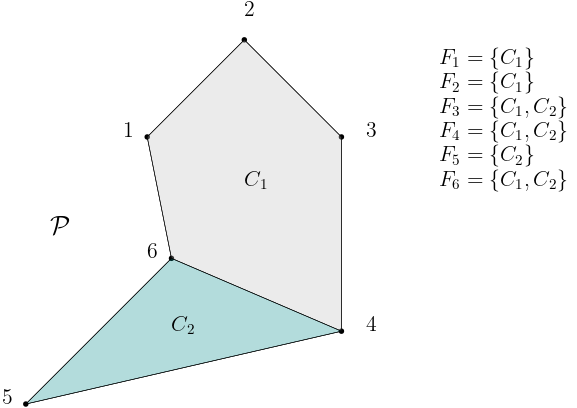
\includegraphics[width=0.7\textwidth]{literature/ghosh-eg.png}
    \caption{Example run of the Algorithm of Ghosh \cite{GHOSH2010718} with polygon $P$ divided into two convex components $C_1$ and $C_2$. The resulting guard set is $S = \{6\}$.}
    \label{fig:ghosh}
\end{figure}

\newpage
\subsubsection{Algorithm of Bhattacharya, Ghosh and Roy}
The algorithm of Bhattacharya et al. \cite{bhattacharya2016approximability} runs in $O(n^2)$ time and yields a 6-approximation for computing the minimum vertex guard for weak visibility polygons without holes. 

It begins by choosing two neighbours $u$ and $v$ as parents for every vertex in $P$. It then computes the Shortest Path from each pair of parents $(u, v)$ to every other vertex in $P$. The Shortest Path is a path between two vertices such that the distance between them is minimal. If all distances between two adjacent vertices are the same, then the length of the path corresponds to the number of edges between the vertices. The Shortest Path from a pair of vertices $(u, v)$ to any other vertex $w$ is the length of the minimum path between $u$ and $w$, and $v$ and $w$.

Then, all vertices that can be reached from $u$ and $v$ are unmarked. In increasing angular order from $\overline{uv}$, every vertex $w \in P$ is checked for visibility from $u, \text{ and } v$. If all vertices $w$ are visible, then $u, \text{ and }v$ are added to $S$. Otherwise, $w$ is added to $S$ and the procedure continues with $w$ as the starting node. All vertices that become seen from $S$ are marked. At the end, the algorithm checks whether the vertices in $S$ have overlapping visibility regions, and duplicates are removed.

An example run of the algorithm is depicted in Figure \ref{fig:bhaca}. Let $P$ be the polygon in question, and its boundary vertices $\mathcal V = \{a, b, c, d, e, f\}$. The algorithm starts with vertices $a$ and $c$ as parents of $b$. Clockwise, vertex $d$ is visible from $\overline{ac}$, but $e$ is not. For this reason, $e$ is added to the guard set $S$, and vertices $d$ and $f$ are chosen as the new parents. In increasing angular order, all vertices $a, b, c, e$ are visible from $\overline{ef}$, so $d$ and $f$ are added to $S$. Since the visibility regions of $d$ and $f$ coincide ($Vis(d) = Vis(f)$), and the visibility region of $e$ is included in that of $d$ and $f$ ($Vis(e) \subseteq Vis(d) \subseteq Vis(f)$), $e$ and $d$ can be removed from $S$. As such, the final guard set becomes $S = \{f\}$.

\begin{figure}[h!]
    \centering
    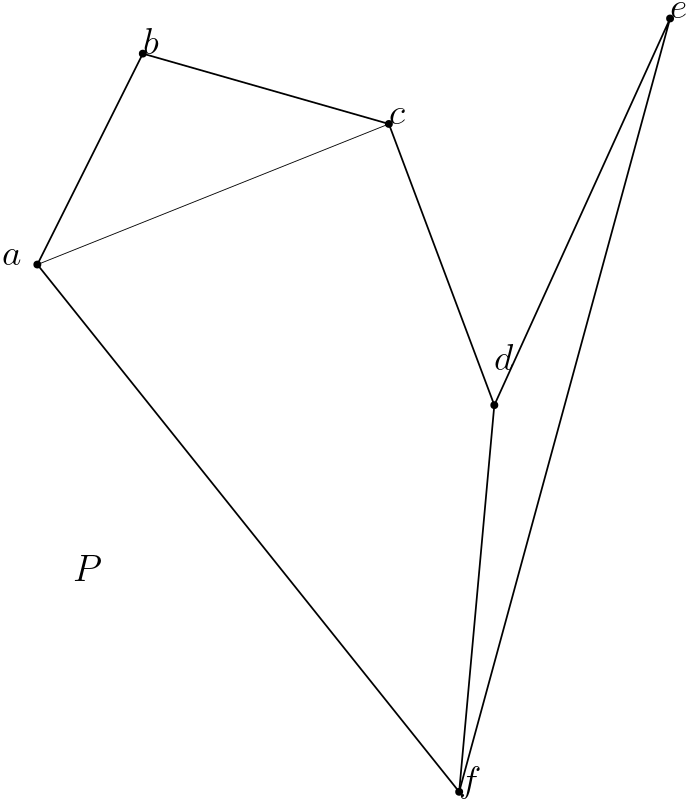
\includegraphics[width=0.5\textwidth]{literature/bacha-eg.png}
    \caption{Example run of the Algorithm of Bhattacharya et al. \cite{bhattacharya2016approximability} for polygon $P$. The final guard set is $S = \{f\}$.}
    \label{fig:bhaca}
\end{figure}

\newpage
\subsubsection{New Algorithm}
The algorithm introduced by Maleki and Mohades is focussed on polygons with large number of vertices $n$ and different amounts of reflex vertices $r$. If the number of reflex vertices is significantly lower than the total number of vertices ($r \leq \log \log n$), guards are placed at all reflex vertices. Otherwise, they are placed according to the algorithm of Ghosh \cite{GHOSH2010718}.

\subsubsection{Experiments}
Algorithms of Ghosh \cite{GHOSH2010718} and Bhattacharya et al. \cite{bhattacharya2016approximability} are tested on weak visibility polygons, and the newly introduced algorithm is tested on simple polygons. 

Let Procedure 1 be a procedure for generating weak visibility polygons that is illustrated in Figure \ref{fig:weak}: given two points $p = (k, 0), q = (-k, 0)$,  $n$ random points $\{x_1, ..., x_n\}$ sorted on the distance from $p$ on $\overline{pq}$, $n$ sorted random angles $\{\alpha_1, ..., \alpha_n\} \in  (0, \pi)$, and $n$ vertices $\{y_1, ..., y_n\}$ are created by shooting $n$ rays at the corresponding angle $\alpha_i, \forall x_i$. Then, $n$ reflex vertices $\{z_1, ..., z_n\}$ are added in the quadrilateral formed by vertices $x_iy_iy_{i + 1}x_{i + 1}$. The figure is accredited to \cite{maleki2022implementation}.

\begin{figure}[h!]
    \centering
    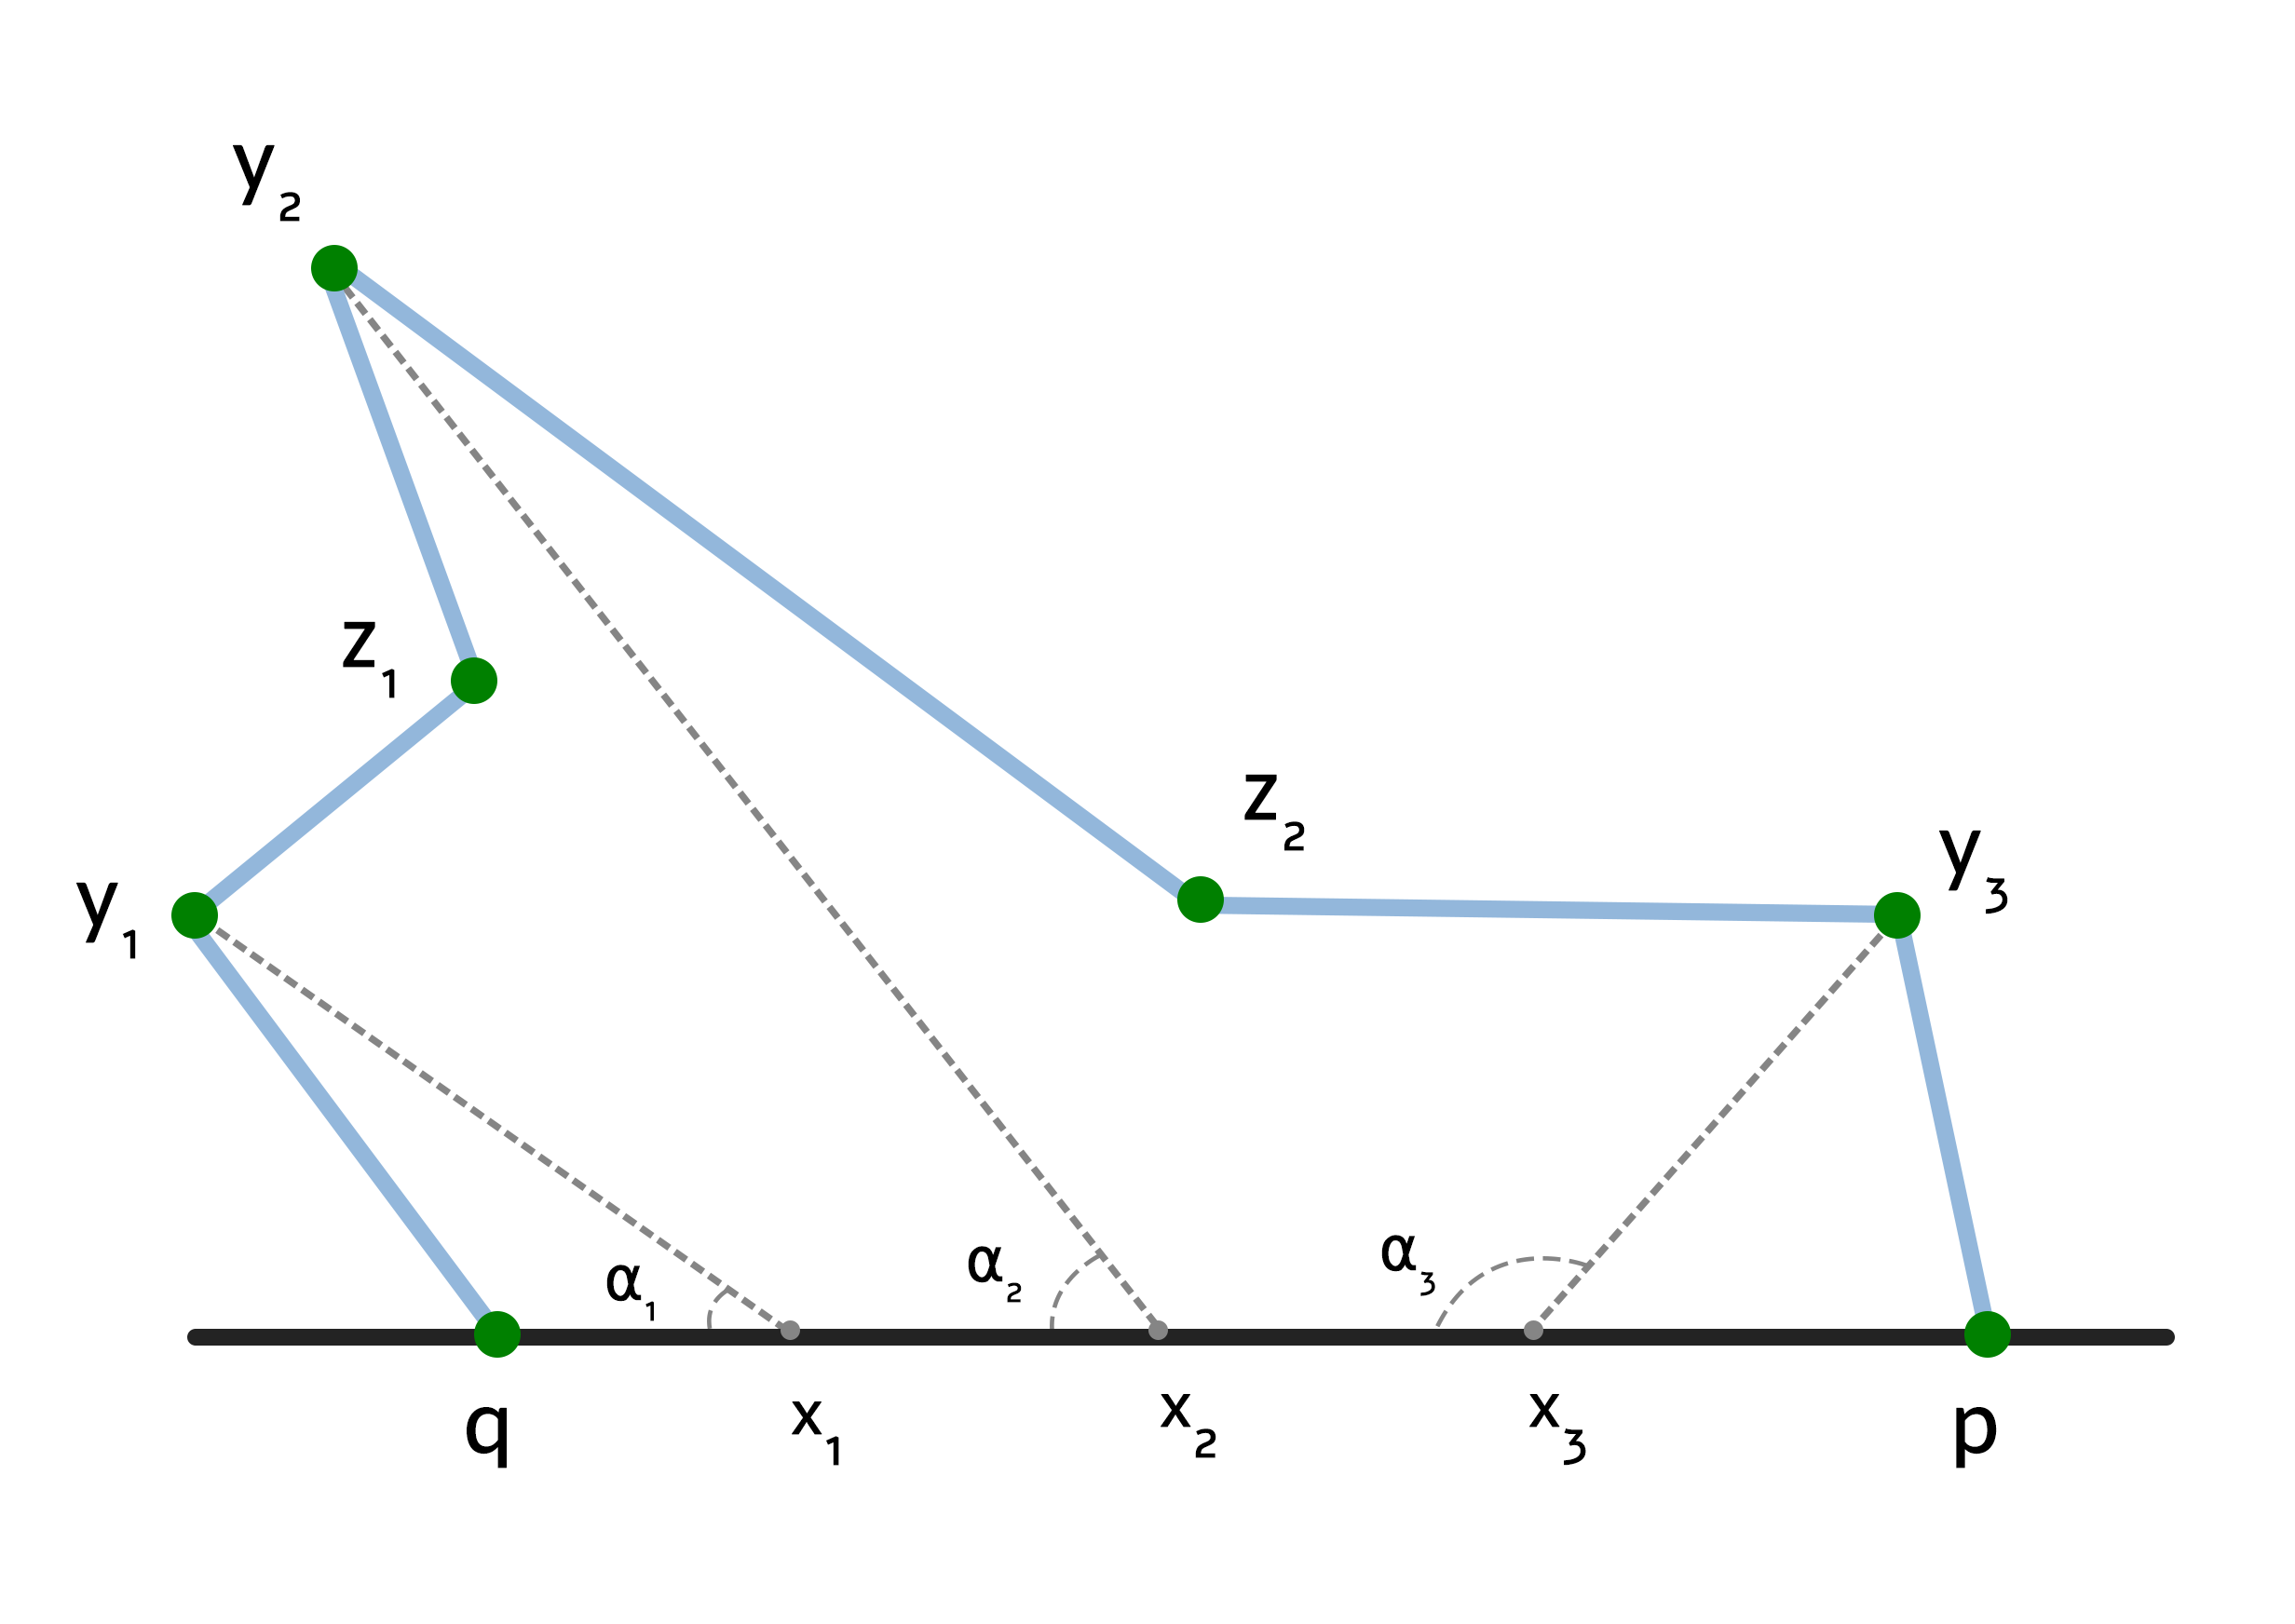
\includegraphics[width=0.6\textwidth]{literature/weak.png}
    \caption{Generated weak visibility polygon for $n = 3$ \cite{maleki2022implementation} through Procedure 1.}
    \label{fig:weak}
\end{figure}

The algorithms of Ghosh \cite{GHOSH2010718} and Bhattacharya et al. \cite{bhattacharya2016approximability} were tested using polygons generated by Procedure 1 with $n \in \{10, 11, ..., 15\}$ vertices and $r \in \{2, 3\}$ reflex vertices. The results suggest that for low values of $n$ and $r$, the algorithm of Ghosh \cite{GHOSH2010718} performs better when using the number of guards as evaluation criteria. 
% Its constant time approximation in the small case contrasts with the constant approximation of the algorithm of Bhattacharya \cite{bhattacharya2016approximability}.
Similarly, the algorithm of Ghosh \cite{GHOSH2010718} performed better both when tested on a weak visibility polygon with low $n = \overline{10, 15}$ and $\frac n 2 \leq r$, and when tested with large $n \in \{100, 400\}$.

Secondly, let Procedure 2 be a procedure for generating simple polygons with custom number of reflex vertices $r$ is devised in Figure \ref{fig:arbitrary}. The figure was taken from \cite{maleki2022implementation} and annotated to suit the explanations in these summaries. Starting from a simple convex polygon $P$ with $n$ vertices ($u, v, x1, x2, ..., x7$), $P$ is triangulated such that every triangle has a joint edge with its boundaries; $r$ reflex vertices ($r1, r2, r3$) are randomly added inside $P$, and the boundaries outside of the reflex vertices are moved such that all $r$ points are now forming boundaries. 

\begin{figure}[h!]
    \centering
    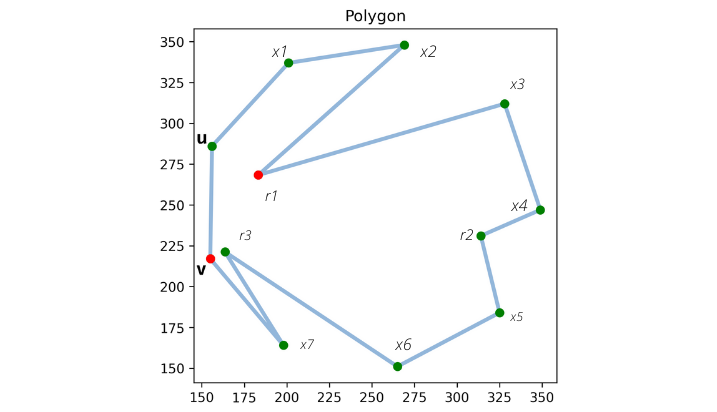
\includegraphics[width=0.7\textwidth]{literature/concave_test.png}
    \caption{Generated simple polygon $P$ for $n = 12, r = 3$ \cite{maleki2022implementation} through Procedure 2.}
    \label{fig:arbitrary}
\end{figure}

The new algorithm is tested on simple polygons constructed as mentioned by starting from low $r$ and gradually increasing it. The results are reported positively in the sense that the $|S|$ always remains close to the optimal, as a 2-approximation solution.

Therefore, through the newly implemented algorithm, Maleki and Mohades \cite{maleki2022implementation} testify that the algorithm of Ghosh \cite{GHOSH2010718} performs like a constant approximation in practice, and often better than its theoretical bound when tested on complex simple polygons.
% - guards placed on vertices = vertex guards
% - no restrictions = point guards
% - $P$ is called weak visibility polygon if every point in $P$ is visible from some point of an edge
% - the problem of computing a min number of guards is NP-hard
% - $O(n^4)$ approximation algorithm for computing $S$ (1)
% - $O(n^2)$ 6-approximation algorithm for vertex \subsection{Implementation of Polygon Guarding Algorithms for Art Gallery Problems \cite{maleki2022implementation}}
% - guards placed on vertices = vertex guards
% - no restrictions = point guards
% - $P$ is called weak visibility polygon if every point in $P$ is visible from some point of an edge
% - the problem of computing a min number of guards is NP-hard
% - $O(n^4)$ approximation algorithm for computing $S$ (1)
% - $O(n^2)$ 6-approximation algorithm for vertex guarding a weak vibisility $P$ with no holes (2)
% - implementation of algorithms and testing on weak visibility polygons
% - generating arbitrary weak visibility polygons *add algorithm* and testing them with $n = \overline{10, 15}$ and $r \in \{2, 3\}$ reflex vertices
	% - for low value of $n$ and $r$, it is better to use Algorithm 1 for minimising the number of vertex guards; since algorithm 2 is a constant approximation algorithm, algorithm 1 performs like a constant time approximation algorithm for small values of $n$ and $r$ experimentally
	% - since the criteria of minimisation is the number of guards rather than the running time which is a one-time affair unlike online algorithms, algorithm 1 is preferable even for weak visibility polygons
% - generating arbitrary weak visibility polygons and testing them with $n = \overline{10, 15}$ and $r$ reflex vertices close to the number of convex vertices
	% - for a low value of $n$ and $\frac n 2 \leq r$, algorithm 1 is better for guarding a weak visibility polygon with a min number of guards, because when the number of reflex vertices increases, the number of the diameter of the polygon and convex components decrease
% - generating arbitrary weak visibility polygons and testing them with large $n$
	% - algorithm 1 is better for guarding a weak visibility polygon with min number of guards, because it uses less guards than algorithm 2
% - generating arbitrary simply polygons *add algorithm* (Ghosh)
% - if $r << n$ , then the size of the optimal guard set is $\approx r$  => the number of edges $E$ in the visibility graph of such simple polygons is $O(n^2)$ => choose a small number $\log \log n$ as an upper bound for $r$ so that $r$ and optimal are close
% - if $r - c \leq \log \log n$, $c$ - small constant, then we place guards at all reflex vertices for guarding a simple polygon $P$, otherwise we place guards using the method of algorithm 1
% - even if $E$ reduces, the chosen guard sets remains close to the optimal and the algorithm assigns no more than twice the optimal number of guards
% => Ghosh's idea works better in practice and performs like a constant approximation algorithmalgorithm 2 is a constant approximation algorithm, algorithm 1 performs like a constant time approximation algorithm for small values of $n$ and $r$ experimentally
	% - since the criteria of minimisation is the number of guards rather than the running time which is a one-time affair unlike online algorithms, algorithm 1 is preferable even for weak visibility polygons
% - generating arbitrary weak visibility polygons and testing them with $n = \overline{10, 15}$ and $r$ reflex vertices close to the number of convex vertices
	% - for a low value of $n$ and $\frac n 2 \leq r$, algorithm 1 is better for guarding a weak visibility polygon with a min number of guards, because when the number of reflex vertices increases, the number of the diameter of the polygon and convex components decrease
% - generating arbitrary weak visibility polygons and testing them with large $n$
	% - algorithm 1 is better for guarding a weak visibility polygon with min number of guards, because it uses less guards than algorithm 2
% - generating arbitrary simply polygons *add algorithm* (Ghosh)
% - if $r << n$ , then the size of the optimal guard set is $\approx r$  => the number of edges $E$ in the visibility graph of such simple polygons is $O(n^2)$ => choose a small number $\log \log n$ as an upper bound for $r$ so that $r$ and optimal are close
% - if $r - c \leq \log \log n$, $c$ - small constant, then we place guards at all reflex vertices for guarding a simple polygon $P$, otherwise we place guards using the method of algorithm 1
% - even if $E$ reduces, the chosen guard sets remains close to the optimal and the algorithm assigns no more than twice the optimal number of guards
% => Ghosh's idea works better in practice and performs like a constant approximation algorithm
\newpage
\subsection[An Algorithm with Performance Guarantees]{A Practical Algorithm with Performance Guarantees for the Art Gallery Problem}
Hengeveld and Miltzow \cite{DBLP:journals/corr/abs-2007-06920} introduce the idea of vision-stability, and describe an iterative algorithm that guarantees to find the optimal guard set for every vision-stable polygon in order to address the Art Gallery Problem \cite{o1987art}. Additionally, it proves that the set of vision-stable polygons admits an FPT algorithm when parametrised by the number of vertices visible from a chord of the polygon, and gives a one-shot algorithm for that matter.

Hengeveld and Miltzow \cite{DBLP:journals/corr/abs-2007-06920} start by introducing the notion of vision-stability (see Figure \ref{fig:vis}). The figure was taken from \cite{DBLP:journals/corr/abs-2007-06920} and annotated to facilitate the understanding of this summary. The authors define guards as ``enhanced'' if they can ``see around the corner'' by an angle of $\delta$ ($vis_\delta(q)$), or ``diminished'' if their vision is ``blocked'' by reflex vertices by an angle of $\delta$ ($vis_{-\delta}(q)$). As such, the size of the minimum $\delta$-guarding set is defined as $opt(P, \delta)$. A polygon $P$ has vision-stability $\delta$ if the optimal number of enhanced guards is the same as the optimal number of diminished guards for that matter ($opt(P, -\delta) = opt(P, \delta)$). 

\begin{figure}[h!]
    \centering
    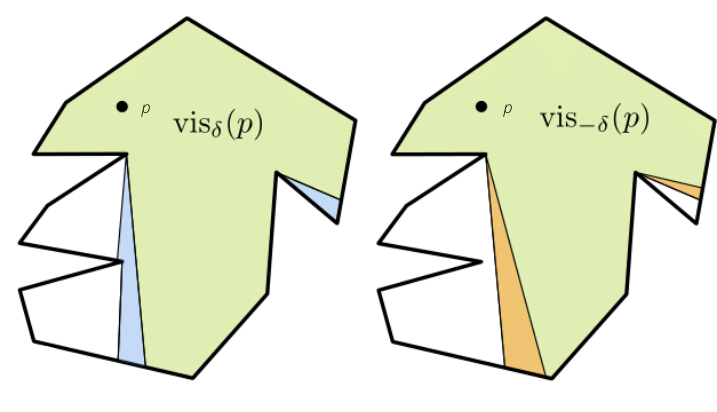
\includegraphics[width=0.5\textwidth]{literature/vis_delta.png}
    \caption{Enhanced ($vis_\delta(q)$) and diminished ($vis_{-\delta}(q)$) visibility regions of the one point $q$ \cite{DBLP:journals/corr/abs-2007-06920}.}
    \label{fig:vis}
\end{figure}

The core idea of Hengeveld and Miltzow's approach is to discretise the problem in order to improve the computation time. In this way, only a subset of potential guards and points to be guarded from $P$ would be considered. In order to do so, they introduce the notions of a candidate guard set $C$ and a witness set $W$. The role of the candidate guard set $C$ is to discretise the guard searching space. As such, we can find an upper bound $opt[C]$ on the final guard set. Thus $C$ is ``pretty close'' on the actual optimum guard set $opt$. The candidate guard set $C$ is then initialised with a subset of all the potential guards. The guards that are included should have their visibility regions overlap as little as possible. Similarly, the witness set $W$ discretises the space of the guards' visibility regions. At initialisation time, $W$ contains a subset of all vertices and faces of $P$. It is important to also include faces in $W$. In this way, we account for the fact that if a point $q$ is included in a face $f$, then $f$ sees at least as much as $q$. So, we can determine an approximation of how much more $f$ sees when compared to $g$. Thus, by adding the face as a witness, we are creating a discretisation of the space containing a superset of possible guard positions.

Firstly, rays are shot from every reflex vertex such that the angle between any two rays is at most $\delta$, as observed in Figure \ref{fig:rays}, as taken from \cite{DBLP:journals/corr/abs-2007-06920}. All the intersection points of the rays within $P$ define the candidate guard set $C$, together with the faces they are part of. A witness guard set $W$ is then defined by picking an arbitrary interior point of every face of $P$, together with all faces of $P$. In this way, the problem can be discretised in a way in which the solution to the discretised problem are also solutions to the continuous problem.

\begin{figure}[h!]
    \centering
    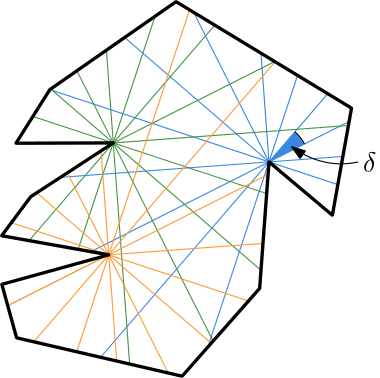
\includegraphics[width=0.3\textwidth]{literature/Shooting-1.png}
    \caption{Shooting rays from all reflex Vertices with angles between them at most $\delta$ \cite{DBLP:journals/corr/abs-2007-06920}.}
    \label{fig:rays}
\end{figure}

\newpage
\subsubsection{One-Shot Vision-Stable Algorithm}
At first, an Integer Program (IP) is built and named the One-Shot Vision-Stable Algorithm. It computes the minimum number of point guards in polynomial time in a vision-stable polygon $P$ with  vision-stability $\delta$ and $r$ reflex vertices. The guards are encoded by binary integers, and linear equations and inequalities are used to encode visibility. Assuming that $\delta$ is part of the input, the algorithm returns the optimal solution only if the vision-stability of $P$ is larger or equal to $\delta$. The one-shot vision-stable algorithm is reliable, as it also verifies that its result is an optimal solution. 

Let $f_1$ be the optimisation fuction of the IP. The function $f_1$ uses variables $[[c]]$ for every candidate $c \in C$, and $[[w]]$ for every witness $w \in W$. Its role is to count the number of guards that are used with the purpose of minimising this number. Additionally, it makes use of parameter factor $1 + \varepsilon$  to ensure that vertex candidates are preferred over face candidates. By choosing $\frac 1 \varepsilon = |C| + |W| + 1$, we ensure that $\varepsilon$ is sufficiently small. As such, the optimisation function $f_1$ of the IP is 
$$f_1 = \sum_{c \in \text{vertex}(C)} [[c]] + (1 + \varepsilon)\sum_{c \in \text{face}(C)} [[c]] + \varepsilon \sum_{w \in \text{face}(W)} [[w]].$$
For every witness $w$, its visible set of candidates are denoted as $vis(w)$, where $face$ and $vertex$ refer to whether the candidate is a face or a vertex, respectively.

Additionally, let $\text{vis}(w)$ be the set of candidates that see witness $w \in W$ completely. For every vertex-witness $w \in \text{vertex}(W)$, we formulate a constraint such that all $w \in \text{vertex}(W)$ is seen: $$\sum_{[[c]] \in vis(w)} c \geq 1, \forall w \in \text{vertex}(W).$$ We similarly formulate a constraint for every face-witness $w \in \text{face}(W)$. However, we add $[[w]]$ as a variable to relax it, so that the focus is placed on first seeing all vertex-witnesses $$[[w]] + \sum_{[[c]] \in vis(w)} c \geq 1, \forall w \in \text{face}(W).$$

% for each vertex and face witness $w$ to be respectively seen by all candidates from $vis(w)$ is added. 
% % \begin{equation}
% 	\begin{align*}
% 		\sum_{c \in \mathit{Vis}(w)} c &\geq 1, \forall w \in \text{vertex}(W) \\
% 		w + \sum_{c \in \mathit{Vis}(w)} c &\geq 1, \forall w \in \text{face}(W).
% 	\end{align*}
% \end{equation}

Nonetheless, the one-shot vision-stable algorithm proves to be too slow for practical reasons. The bottleneck is however not solving the IP in itself, but computing visibilities. Hence, an iterative vision-stable algorithm is devised, that is faster and retains similar performance guarantees. 

\subsubsection{Iterative Vision-Stable Algorithm}
Starting with the smaller sets of candidates $C$ and witnesses $W$, another IP is deployed in order to find a minimum guard set $S \subseteq C$ that sees all vertex-witnesses. This algorithm is then called the Iterative Vision Stable Algorithm, as it changes $C$ and $W$ in each iteration.

As the Iterative Vision Stable Algorithm is also named the Big IP, it also has an objective function $f_2$. The function $f_2$ minimises the number of face-guards used in $S$ and the number of unseen face-witnesses. If $S$ contains only point guards and sees all face-witnesses, the algorithm reports the optimal solution by using the One-Shot IP. As such, $f_2$ assures that all witnesses $w$ are seen by their set of candidates $vis(w)$, and enforces that only the number of guards $s$ resulted from the One-Shot IP is used. The optimisation function with its constraints of the Big IP becomes
\begin{align}
	f_2 &= \sum_{x \in splittable(W \cup C)} [[x]] \label{eq:f2}\\
	\sum_{[[c]] \in C} c &= s, s \in \mathbb Z, s \text{ the number of used guards in the One-Shot IP} \\
	\sum_{[[c]] \in vis(w)} c &\geq 1 \\
	1 - (\varepsilon \sum_{[[c]] \in vis(w)} c) &\geq [[w]].
\end{align}

If not all point guards are used, or not all face-witnesses are seen, the faces of $P$ are split (discretised). Then the algorithm continues to the next iteration. The One-Shot IP is then used as soon as all faces are deemed unsplittable (they have reached a certain granularity~$\lambda$). 

% At first, the new IP builds on the One-Shot IP by forming $W^* \subseteq W$ as a critical witnesses set with only 10\% randomly selected vertices from $W$. The witness set $W^*$ is expanded throughout the iterations with the witnesses that are not seen by the optimal solution at that moment. The new IP is referred to as the Big IP.
% Then, the Big IP receives a secondary objective function $f_2$ (Equation \ref{eq:f2}). The function $f_2$ minimises the number of face-guards used in $S$ and the number of unseen face-witnesses. If $S$ contains only point guards and sees all face-witnesses, the algorithm reports the optimal solution by using the One-Shot IP. Otherwise, the faces of $P$ are split (discretised) and the algorithm continues to the next iteration. The One-Shot IP is then used as soon as all faces are deemed unsplittable (they have reached a certain granularity $\lambda$). In that case, the Big IP is run again. The Big IP consists thus of a similar objective and constraints as the One-Shot Vision-Stable IP: besides assuring that all witnesses $w$ are seen by their set of candidates $vis(w)$, it also enforces that only the number of guards $s$ resulted from the One-Shot IP is used, as follows: 


Inspired by the Iterative Algorithm, an FPT algorithm for the Art Gallery Problem can be created. In this case, the FPT algorithm would have as parameter of chord-visibility width. Given a chord $c$ of $P$, we count the number $n(c)$ of vertices visible from $c$. The chord-visibility width of $P$ ($cw(P)$)  is the maximum $n(c)$ over all possible chords $c$. By using this measure, it is possible to describe the local complexity of a polygon: many synthetic arbitrary polygons have much smaller chord-visibility width than they have reflex vertices, and polygons constructed with hardness reductions have the chord-visibility width proportional to the total number of vertices. 

\subsubsection{Experimental Results}
The previously introduced algorithms are tested experimentally in terms of their running times and solution quality with respect to the input size, chord-visibility width and vision-stability of the input polygons $P$. The tests were run on 30 instances of arbitrary simple polygons of sizes 60, 100, 200 and 500 vertices. The algorithms have been implemented both with the theoretical performance guarantees $\mathcal T$ (if no solution is found in $\mathcal T$, abort) and with the practical optimisation of critical witnesses.

When running the Iterative Algorithm with optimisations, reasonable practical results were found: all tested instances were solved to optimality, although the overall running time was not improved when compared to state-of-the-art algorithms. The median running time was also lower than the average running time. This could be accounted for by the sensitivity of the algorithm to the vision-stability of a polygon. Thus, a few polygons that are hard to solve (have low vision-stability) outweigh the rest of the running times.

The Iterative Algorithm without optimisations was on the 60 vertices instance and with the theoretical limit $\mathcal T$ as a safe guard. A solution was found in an efficient manner (within an hour) only for 25 out of 30 instances. For the rest of the 5 instances, the Big IP performed unnecessary splits, which negatively influenced the running times.

Additionally, the correlation between the granularity $\lambda$ of the input polygon was tested for the iterative algorithm with performance guarantees $\mathcal T$. There appeared to be a strong correlation between the running times and $\lambda$. Thus, lower granularity implied a shorter running time.

In terms of the convergence to the optimal solution, the iterative algorithm with optimisations has been used to show the fast convergence in the first few iterations. The speed of the convergence slows down as the algorithm nears its end due to the increasing number of candidates and witnesses that are added to $C$ and $W^*$, respectively, in the later iterations. Nonetheless, it appears that computing the visibility area of the polygon is still the bottleneck in the algorithm's performance.



% _practice-theory gap_; $\exists \mathbb{R}$-complete
% - encode guards by real numbers and use polynomial equations and inequalities to encode visibility
% - optimal solutions found on synthetic instances of up to 5k vertices => discretise the problem and hope that the discretised problem also gives the optimal solution to the original problem
	% - generate a _candidate_ set $C$ and a _witness_ set $W$, compute the optimal way to guard $W$ using the min number of guards in $C$
	% - more candidates and witnesses are generated until the optimal solution is found
	% - find a min guard set $G \subseteq C$ that sees all vertex-witnesses
	% - secondary objective function: minimise the number of face-guards used in $G$ and the number of unseen face-witnesses
	% - if $G$ contains only point guards and sees all face-witnesses => optimal solution; otherwise it refines $\mathbb{A}$ and goes to the next iteration
% - given a closed simply polygon $P$ we say 2 points $p, q$ see each other if the segment $seg(p, q)$ is fully contained in $P$
% - the Art Gallery Problem seeks a min size set $G \subset P$ of guards that sees $P$ completely
% - notion of _vision-stability_
	% - consider an _enhanced_ guard that can see "around the corner" by an angle of $\delta$ or a _diminished_ guard whose vision is by an angle of $\delta$ "blocked" by reflex vertices
	% - a polygon $P$ has vision-stability $\delta$ if the optimal number of enhanced guards to guard $P$ is the same as the optimal number of diminished guards to guard $P$
	% - shoot rays from every reflex vertex, s.t. the angle between any 2 rays is at most some given angle $\delta$; all intersection points of the rays within the polygon $P$ define our candidate set $C$
	% - $vis_\delta(p)$ - enhanced visibility
	% - $vis_{-\delta}(p)$ - diminished visibility regions of points
	% - $opt(P, \delta)$ - size of the min $\delta$-guarding set
	% - $opt(P, -\delta) = opt(P, \delta)$ - vision-stability
	% - _visibility-enhancing region_ $A = A(q, r, \delta)$
	% - don't know how to test it for a specific value $\delta$
% - _one-shot vision-stable_ algorithm that computes an optimal guard set for vision-stable polygons using polynomial time and solving one IP - finds the optimal solution for every vision-stable polygon
	% - the bottleneck is not solving the IP, ol
		% 	- normal protocol - square splits only if the face is incident to more than one reflex vertex; choose angular split with probability 0.8, and the other two remaining split types with equal probabilities; in case a split is impossible, we will try the two other splits, before deciding that a face is unsplittable
		% 	- square spthms
	% - the Art Gallery Problem is in NP for vision-stable polygons
	% - _reliable_ - even if the input polygon is not vision-stable, the reported result is correct
	% - refine by splitting appropriate faces
	% - work with _critical witnesses_
	% 	- initialise the critical witness set $W^*$ by randomly picking 10\% of vertices and faces, for each weak visibility polygon
	% 	- compute all the vertices and faces that the IP $G$ sees (the sets of unseen face-witnesses and vertex-witnesses), then randomly choose a small constant size subset of vertices and faces from $U$ that we add to $W^*$ - find a good balance between adding too few critical witnesses and too many
	% 	- every time we update the critical witness set, rerun the IP to check if we can find a better solution given the critical witnesses; we keep adding to the critical witness set as long as there are unseen witnesses left that are not marked as critical; check if we need to update the new critical witness set again using the new-found guard set (critical cycles); repeat until we find a guard set that can see the entire polygon -> split the faces and continue with the next iteration
	% 	- we do not need to compute all the visibilities between all the candidates and all witnesses; compute all visibilities between the critical witnesses $W^*$ and candidates $C$ and then all visibilities between the guards $G$ and the witnesses $W$
	% 	- _delayed critical witness protocol_ - use critical witnesses and add all faces, which have a power larger than the granularity $\sqrt \lambda$ 
	% - _weak visibility polygon tree_ - exploit low local complexity in order to reduce the number of visibility queries to be answered
		% - start with an arbitrary edge $e$ on the boundary of $P$ -> compute the weak visibility polygon $vis(e)$ of $e$ which is the root of $T$: $\forall e'$ of $vis(e)$ which is not part of the boundary of $P$, we compute the weak visibility polygon $vis(e')$ w.r.t. the polygon $P - vis(e)$ => children of $vis(e)$
		% - $\forall$ node of $T$ is a weak visibility polygon $W$ of some defining chord $c$ => $c$ splits $P$ into 2 polygons $Q$ and $Q'$; the weak visibility polygon $W$ is completely contained in either $Q$ or $Q'$ (consider each node of $T$) to be closed and contain its boundary
		% - initialisation: construct an arrangement $A$, where we add defining chords $c$ of the weak visibility polygon tree to $A$, shot horizontal and vertical rays from each reflex vertex, stop as soon as it hits the boundary or another edge of $A$
		% - splits:
		% 	- square splits - divide a face using a horizontal and vertical segment, s.t. the height and the width of the new faces are halved
		% 	- angular splits - shoot rays from a reflex vertex as to reduce the power of the face
		% 	- reflex chord splits - do them if no other type of split is possible
		% 	- extension splits - given a reflex vertex $r$, we can consider the rays with apex $r$ parallel to the two incident edges of $r$
		% 	- unsplittable faces - the face is incident to at most one reflex vertex + no reflex chord or extension split is possible + the face is not splittable by angular splits of granularity $\lambda$ 
		% - protocol
		% 	- normal protocol - square splits only if the face is incident to more than one reflex vertex; choose angular split with probability 0.8, and the other two remaining split types with equal probabilities; in case a split is impossible, we will try the two other splits, before deciding that a face is unsplittable
		% 	- square split protocol - always use square splits
% - building the IP
	% - normal IP - one-shot IP, only adds constraints and variables for critical witnesses
		% - if $G$ contains only vertex-guards and we checked that $G$ sees the entire polygon, then the algorithm reports $G$ as the optimal solution; else continue with the next iteration; else use the big IP
	% - big IP - find a solution with at least one unsplittable face, maximise the number of splittable faces that are used
% - granularity update protocol - replace $\lambda$ by $\frac \lambda 2$ (_normal granularity update protocol_), or by $\lambda^2$ (_accelerated granularity update protocol_) - use almost exclusively the simple IP protocol; accelerated seems to combine the best of both worls
% - given a chord $c$ of a polygon, $n(c)$ number of vertices visible from $c$
	% - _chord-visibility width_ $cw(P)$ of a polygon is the max $n(c)$ over all possible chords $c$
	% - the set of vision-stable polygons admit an FPT algorithm, when parametrised by the chord-visibility width

% - run practical algorithm $\mathbf{P}$ within the running time bound of $\mathbf{T}$(safe-guard), abort if no solution 
% - test the algorithm on several input polygons (30 instances of sizes 60, 100, 200 and 500 vertices) with algorithm that has theoretical performance guarantees and optimised one
% 	- iterative algorithm without safe guards - used critical witness protocol with normal split protocol and simple IP - find optimal solutions for all tested instances, performs similar to other algorithms, but susceptible to the vision-stability of the algorithm
% 	- iterative algorithm with safe guards - no critical witnesses, normal split protocol, normal IP protocol
% 		- efficient solution for 25/30 instances for 60-vertices polygon
% 	- correlation of granularity and running time - min granularity $\lambda$ might not be the best indication of the vision-stability of a polygon (discretisation); random IP splits choice, chord-visibility width influence
% 	- distribution of CPU usage - the running time of the algorithm is dominated by the face-visibility queries combined with the weak visibility decomposition
\section{Theory}
\label{sec:theory}

This section will investigate the theory aspects of solving the Art Gallery Problem using gradient descent. Namely, we will explain what the optimisation function in the context of the Art Gallery problem is, and how it can be solved with gradient descent. We will initially apply gradient descent to only one guard, then extend it to multiple guards.

\subsection{Guarding the Polygon with One Point}

First, we will explore how gradient descent can be applied for the case that we want to guard the polygon using only one guard.

\subsubsection{Gradient Descent}
\label{sec:gradient}

Let $P$ be a polygon and $g = (x, y) \in P$ a guard. We are interested in computing the best direction for moving $g$ inside $P$ such that the visibility area $\mathit{Vis}(g)$ increases. That is, exploring what would be a better position $g'$ to move $g$ to such that $g$ ``sees more'' of the polygon $P$. 

We define $f(g) = \text{Area}(g)$ as the area seen by a guard $g$. Let $\bigtriangledown \text{Area}_r(g)$ be the local change in the area guarded by point $g$ around a reflex vertex $r$ seen by guard $g$, thus $r \in \mathit{Vis(g)}$. Given all reflex vertices $i$, the total (global) change in the area seen by $g$ can be thus summed up to $\text{Area}(g) = \sum_i \text{Area}_i(g)$. Figure \ref{fig:sumf} offers an example for this case for a polygon $P$ and its reflex vertices $r_1$ and $r_2$. The polygon $P$ is guarded by $g$, and its position is modified to $g'$ by a small change $\partial y$ in its $y$-coordinate. The visibility areas of $g$ are $Area_{r_1}$ and $Area_{r_2}$ around reflex vertices $r_1$ and $r_2$, respectively. In this way, the total change in the visibility area of $g$ is computed as $\bigtriangledown \text{Area}(g) = \bigtriangledown \text{Area}_{r_1}(g) + \bigtriangledown \text{Area}_{r_2}(g)$.

Thus, we consider $f(g)$ as the continuous objective function of the Art Gallery Problem. We can then use gradient descent as a method to optimise the objective function $f$. We will define below what the methodology of gradient descent is comprised of.

\begin{figure}[h!]
    \centering
    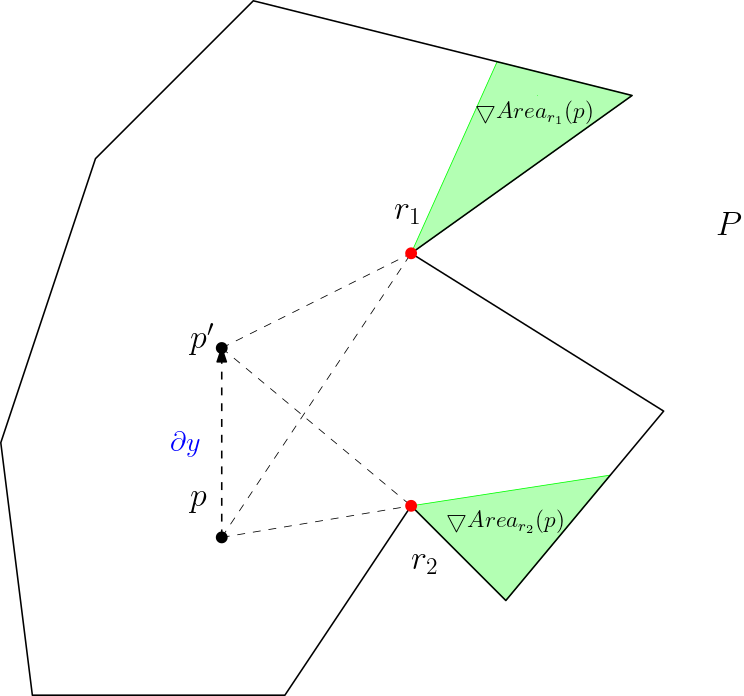
\includegraphics[width=0.4\textwidth]{theory/sumf.png}
    \caption{Global change in the area seen by $g$ when moved by $\partial y$ to a new position $g'$.}
    \label{fig:sumf}
\end{figure}


Let $\bigtriangledown f$ be the gradient of $f$. The gradient then indicates the direction of the steepest descent for the objective function $f(g)$.
The learning rate (step size) $\alpha$ is the size of the steps taken to reach the optimum. It is typically a small value, and it is evaluated and updated based on the behaviour of the optimisation function. 

After the gradient $\bigtriangledown f$ is computed, we can use it to calculate the new optimised position $g'$ of guard $g$: $$g' = g + \alpha\bigtriangledown f.$$


In later sections we will experiment with various learning rates. As such, we will explore how they influence the performance of our algorithm in relation to different test polygons. 

\newpage
\subsubsection{Computing the Gradient}

Given that $f$ is a function that describes the visibility area of a point $g$, we first need to define how its gradient is computed. We will simplify the gradient computation without losing generality. As such, we will rotate the plane with rotation matrix $R$, so that $g$ and any reflex vertex $r$ have the same $x$-coordinate. In this way, we only need to compute the gradient when we vary the $y$-coordinate. The computation of the gradient remains the same regardless of the rotation applied to the plane.


We will use the notation $\frac{\partial f}{\partial y}$ to denote the change in the visibility area $f(g)$ when the plane is rotated and then the $y$-coordinate is modified by a small amount $\partial y \rightarrow 0$. In this way, we define 

\begin{equation}
    \bigtriangledown f = \left(\frac{\partial f}{\partial x}, \frac{\partial f}{\partial y}\right)^\intercal \label{eq:gradient}
\end{equation}

to be the gradient of $f$ given that $P$ is guarded by a point $g$. 

We will now create a canonical geometrical construction that allows us to further define and compute $\bigtriangledown f$. In this case, we consider the normalised length of the gradient as $||~\bigtriangledown~f||~=~1$. This canonical construction is displayed in Figure \ref{fig:gradient}. 
% We will then generalise this case to multiple reflex vertices and guards.

\begin{figure}[h!]
    \centering
    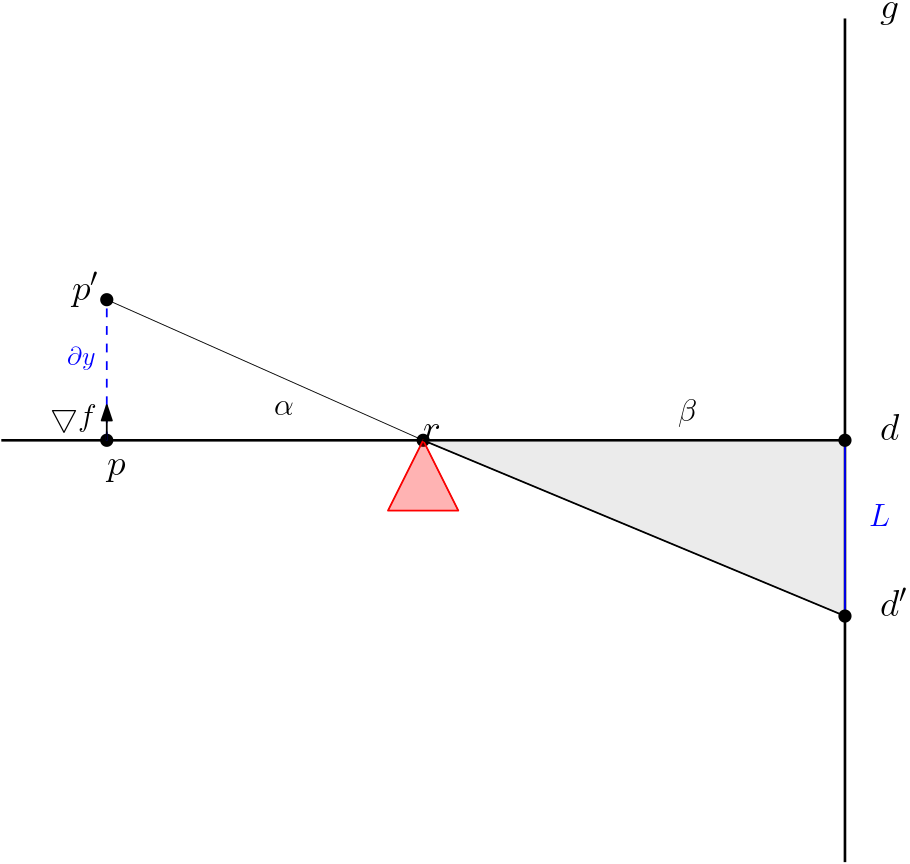
\includegraphics[width = 0.6\textwidth]{theory/gradient2.png}
    \caption{Canonical gradient construction for when the position of $g$ is varied by a small amount $\partial y$ around reflex vertex $r$ to the new position $g'$.}
    \label{fig:gradient}
\end{figure}

Take a boundary line segment of $P$, $r$ a reflex vertex inside $P$ and $g$ a guard whose optimal position we are interested in. The reflex vertex $r$ is seen by $g$. Let $\overline{pr} = a$ be known, and let $\triangle rpp' = \triangle_2$. Similarly, let $b$ be the known distance between $r$ and the polygon boundary in question.


Let $\partial y$ be an extremely small change in the $y$-coordinate of $g$. Let $g'$ be the new position of $g$ given the change $\partial y$. The point $g'$ can see then up to a new point around $r$ on the polygon boundary. Let thus the new observed segment on the polygon boundary be $L$. As such, let $\triangle_1$ denote the increase in the visibility area of $g$ when it moves to position $g'$:

\begin{equation}
    \bigtriangledown \text{Area}_r = \triangle_1. \label{eq:derivative}
\end{equation}

We are now interested in computing how the area seen by guard $g$ increases given the change $\partial y$ in the position of $g$. The distances $a$ and $b$ are known. As such, we aim at expressing the gradient $\bigtriangledown \text{Area}_r$ for point $g$ and reflex vertex $r \in \mathit{Vis}(g)$ using $a$ and $b$. Since $\bigtriangledown \text{Area}_r$ depends on the change in the coordinates of $g$, computing it is tightly connected to the change in the area of triangle $\triangle_1$. We will proceed to calculate the area of $\triangle_1$ below.

Given that triangles $\triangle_1$ and $\triangle_2$ are square triangles, their areas can be calculated as:

\begin{align*}
    \text{Area}_{\triangle_1} &= \frac{b L}{2},\\ 
    \text{Area}_{\triangle_2} &= \frac{a \partial y}{2}.
\end{align*}


Given that $\overline{gg'}$ is parallel to polygon's boundary, we can use Thales's Theorem in triangles $\triangle_1$ and $\triangle_2$ to compute the length $L$: 

\begin{align}
    % \frac{||\overline{pp'}||}{||\overline{dd'}||} &= \frac a b \\
    \frac{\partial y}{L} &= \frac a b \\
    L &= \frac{b \partial y}{a}. \label{eq:L}
\end{align}

So, the area of $\triangle_1$ can be computed:
\begin{align}
    \text{Area}_{\triangle_1} &= \frac{Lb}{2} \\
    &\overset{(\ref{eq:L})}{=} \frac{\frac{b \partial y}{a}b}{2} \\
    \text{Area}_{\triangle_1} &= \frac{b^2 \partial y}{2a}. \label{eq:ardd}
\end{align}

We can now compute the gradient $\bigtriangledown \text{Area}_r$ in a plane rotated by $R$ for a point $g$ and a reflex guard $r$ seen by $g$ as

\begin{align*}
    R\bigtriangledown \text{Area}_r \overset{(\ref{eq:gradient})}{=} &\left(\frac{\partial f}{\partial x}, \frac{\partial f}{\partial y}\right)^\intercal \\
    \overset{(\ref{eq:derivative})}{=} &\left(0, \frac{\text{Area}_{\triangle_1}}{\partial y}\right)^\intercal \\
    R\bigtriangledown \text{Area}_r \overset{(\ref{eq:ardd})}{=} &\left(0, \frac{b^2}{2a}\right)^\intercal.
    % \bigtriangledown \text{Area}_r = &\left(0, \frac{b^2}{2a}\right)^\intercal.
\end{align*}

% Analogously, if we rotate the plane such that $p$ and reflex vertex $r$ have the same $y$-coordinate, the gradient becomes $$\bigtriangledown f = (\frac{b^2}{2a}, 0)^\intercal.$$

Therefore, for all the reflex vertices $r$ guard $g$ can see, the total gradient $\bigtriangledown f$ becomes the sum of all the partial gradients $\bigtriangledown f_r$ as $$\bigtriangledown f = \sum_{i \in R(g)} \bigtriangledown \text{Area}_i, R(g) = \{\text{reflex vertices of } P \text{ seen by }g\}.$$

\subsubsection{Computing the New Guard's Position}
We can now use the coordinates of the gradient $\bigtriangledown f$ to compute the movement direction of the guard $g$ given all the reflex vertices from $P$ seen by $g$. In order to do so, we will use the construction depicted in Figure \ref{fig:vperp}. 

\begin{figure}[h!]
    \centering
    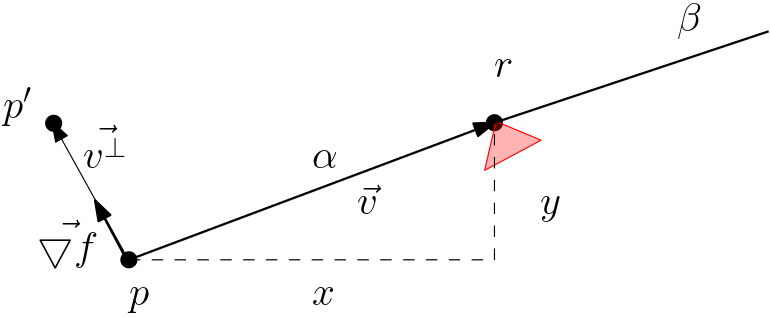
\includegraphics[width = 0.5\textwidth]{theory/v_perp.png}
    \caption{Computing the new position $g'$ of guard $g$ around reflex vertex $r$ based on the gradient $\bigtriangledown f$.}
    \label{fig:vperp}
\end{figure}

Let $\vec v$ be the vector corresponding to the direction of movement from guard $g$ to a reflex vertex $r$, such that $\vec{v} = (r - g) = (x, y)^\intercal$, with norm $||v|| = a$. So, $||\frac{\vec v}{a}|| = 1$.

Let $\vec{v}^\perp  = (g' - g)$ be the vector corresponding to the direction of movement from guard $g$ to its new position $g'$. Vector $\vec v^\perp$ is orthogonal to $\vec{v}$, in the same direction as $\bigtriangledown f$, such that $||\vec{v}|| = ||\vec{v}^\perp|| = a$. We will use the coordinates of $\vec{v}^\perp$ to compute the coordinates of $\bigtriangledown f$ and thus the direction in which $g$ needs to move.

The coordinates of $\vec v^\perp$ can then be computed using the construction from Figure \ref{fig:vsquare}. Since $\vec v^\perp \perp \vec v$, and $g$ and $r$ are on the right-hand side of $\vec v^\perp$, the coordinates of $\vec v^\perp$ will be rotated by $-90^\circ$ so that $\vec v^\perp = (-y, x)^\intercal$. Analogously for the case when $g$ and $r$ are rotated by $180^\circ$ to the left-hand side of $\vec v^\perp$, the coordinates of $\vec v^\perp$ will be rotated by $90^\circ$ to $\vec v^\perp = (-x, y)^\intercal$.

\begin{figure}[h!]
    \centering
    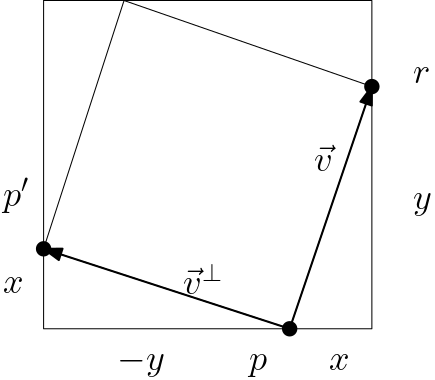
\includegraphics[width = 0.35\textwidth]{theory/v_square.png}
    \caption{Computing the coordinates of $\vec v^\perp$ given the guard $g$ and the reflex vertex $r(x, y)$.}
    \label{fig:vsquare}
\end{figure}

We know that the norm of the gradient is $||\bigtriangledown f|| = \frac{b^2}{2a}$. Since $\bigtriangledown f$ has the same direction as $\vec v^\perp$, we wish to normalise it from the norm of $\vec v^\perp$ with $\frac 1 a$. Therefore, the gradient for guard $g$ and one reflex vertex $r \in \mathit{Vis}(g)$ can be computed as $$\bigtriangledown f = \vec v^\perp \frac{b^2}{2a} \frac 1 a.$$

As mentioned before, the total gradient for guard $g$ and all the reflex vertices $r$ the guard can see is $$\bigtriangledown f = \sum_{r \in R(g)} \bigtriangledown \text{Area}_r, R(g) = \{\text{reflex vertices of } P \text{ seen by }g\}.$$

The new position $g'$ of guard $g$ based on all the reflex vertices it can see is: 
\begin{equation}
    g' = g + \alpha\bigtriangledown f.
    \label{eq:l}
\end{equation}

\newpage
\subsection{Guarding the Polygon with Multiple Guards}
In this subsection we will investigate how to generalise the computation of gradient descent to multiple guards.

\subsubsection{Computing the Gradient for Two Guards}
Let point $g_1$ be the guard we have previously computed the gradient for. Let point $g_2$ be another guard in the polygon. The position of $g_2$ is optimised around reflex vertex $r_2$, as seen in Figure \ref{fig:poly_gradient}. Guard $g_2$ sees a part of the visibility region already seen by $g_1$. Let the shared seen region be $\triangle_2$, and the region that is only visible by $g_1$ be $\triangle_1$.

\begin{figure}[h!]
    \centering
    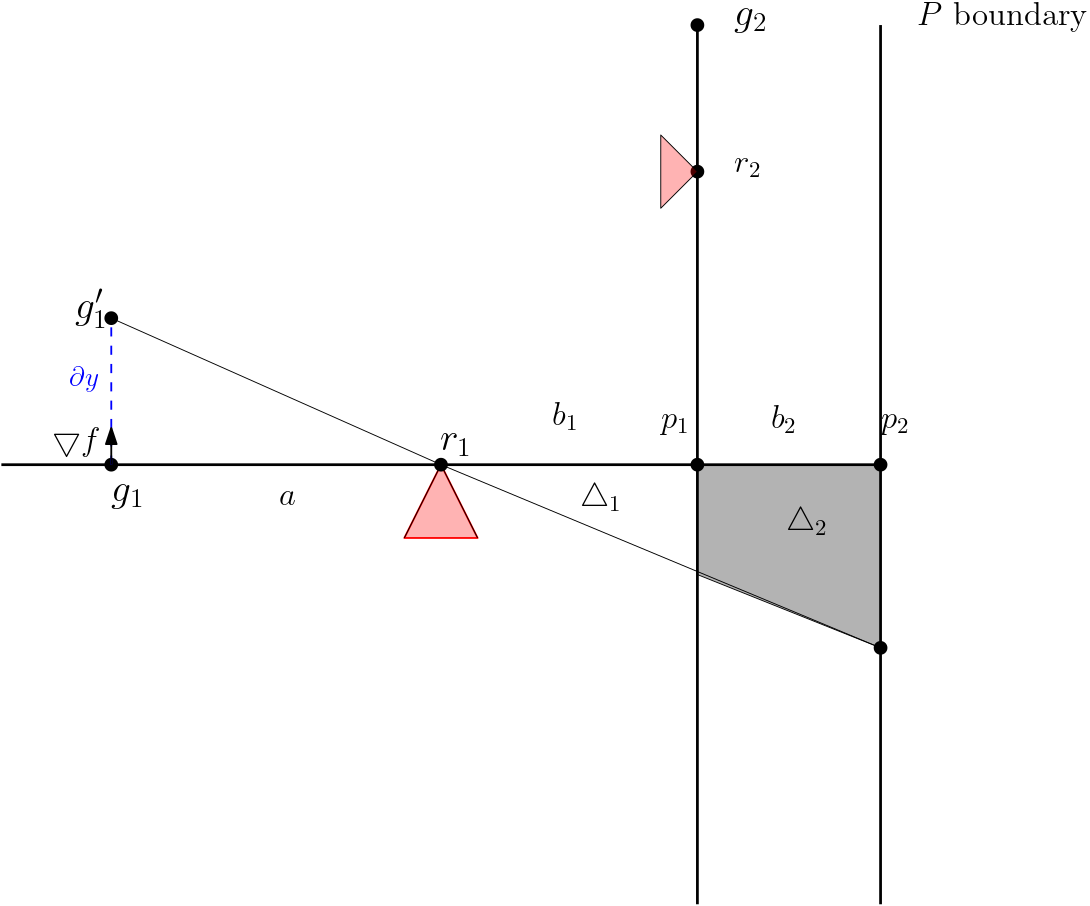
\includegraphics[width = 0.6\textwidth]{theory/gradient3.png}
    \caption{Canonical gradient construction for when the visible area of $g_1'$ is also seen by guard $g_2$.}
    \label{fig:poly_gradient}
\end{figure}

The visibility regions of guards $g_1$ and $g_2$ are computed. Let $p$ be the intersection point between them. Let $d$ be the point seen by $g_1$ on the polygon boundary. Point $p$ divides the segment seen by $g_1$ behind the reflex vertex $r_1$ into two subsegments $\overline{r_1p_1}$ and $\overline{p_1p_2}$. The lengths of the subsegments are $b_1$ and $b_2$, respectively, with $b_1 + b_2 = b$. Recall that $b$ is the distance between the reflex vertex $r_1$ and the polygon boundary. Thus,  $b_2$ corresponds to the length of the shared seen segment.

As before in equation \ref{eq:ardd}, the area seen by $g_1$ is $$\text{Area}_{\triangle_1 + \triangle_2} = (b_1 + b_2)^2\frac{\partial y}{2a}.$$
However, $\triangle_2$ is already seen by guard $g_2$. Since this area is already covered, we are only interested in how $g_1$ can cover the remaining $\triangle_1$. So, we do not need to take $\triangle_2$ into account when computing the gradient of $g_1$. We thus need to subtract the area of $\triangle_2$ from the total area seen by $g_1$. 

First, we need to compute the shared area seen $\triangle_2$ as:
\begin{align}
    \text{Area}_{\triangle_2} &= \text{Area}_{\triangle_1 + \triangle_2} - \text{Area}_{\triangle_2} \\
                              &= (b_1 + b_2)^2\frac{\partial y}{2a} - b_1^2\frac{\partial y}{2a} \\
                              &= \left[(b_1 + b_2)^2 - b_1^2\right]\frac{\partial y}{2a}. \label{eq:multiple_areas} 
\end{align}
Then, we can compute the area $\triangle_1$ seen exclusively by $g_1$ by subtracting the shared area of $\triangle_2$ from the total area seen by $g_1$: 
\begin{align*}
    \text{Area}_{\triangle_1} &= \text{Area}_{\triangle_1 + \triangle_2} - \text{Area}_{\triangle_1} \\
                              &= (b_1 + b_2)^2\frac{\partial y}{2a} - \left[(b_1 + b_2)^2 - b_1^2\right]\frac{\partial y}{2a} \\
    \text{Area}_{\triangle_1} &= b_1^2\frac{\partial y}{2a}. 
\end{align*}

\subsubsection{Computing the Gradient for Multiple Guards}
We can now generalise the gradient computation to $m$ guards and intersection points. Let $g$ be the guard whose position we wish to optimise around reflex vertex $r$ as before. Let the areas highlighted in blue in Figure \ref{fig:general_gradient} be the parts of the visibility region of $g$ that are also seen by the other $m - 1$ guards. Let the visibility region of $g$ intersect other guards' visibility regions in $m$ intersection points $p_1, p_2, ..., p_m$. Let the distance from the reflex vertex $r$ to the intersection points be $b_{11}, b_{12}, ..., b_{m1}, b$.

\begin{figure}[h!]
    \centering
    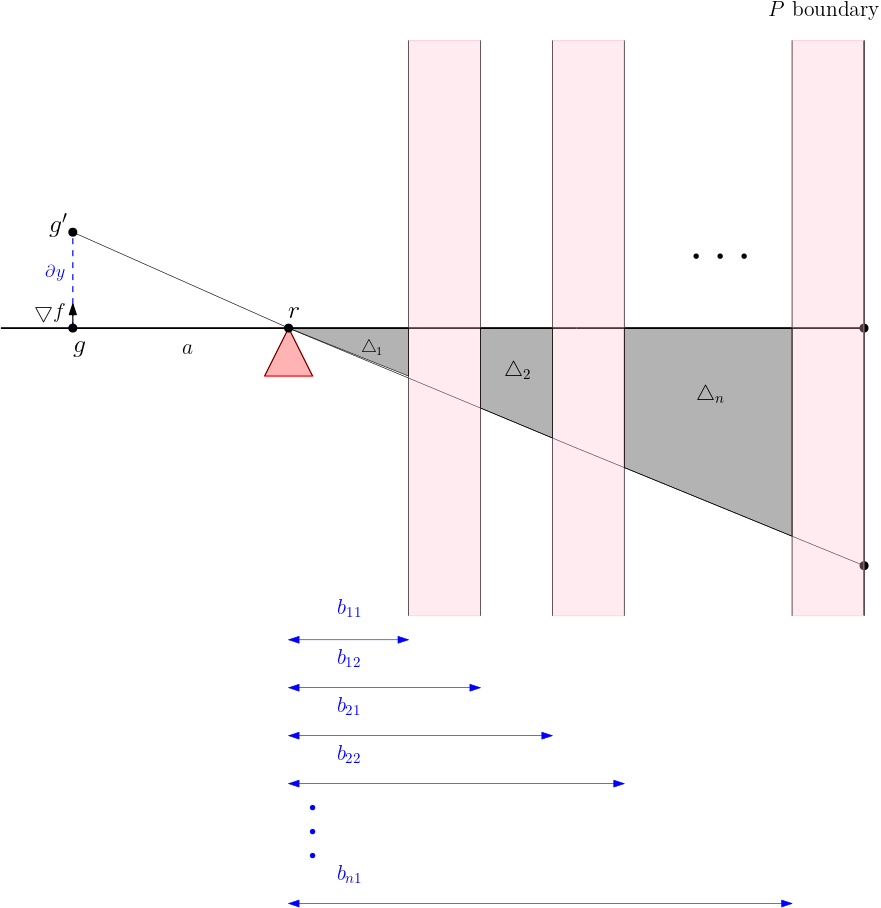
\includegraphics[width = 0.7\textwidth]{theory/gradient4.png}
    \caption{Canonical gradient construction for where the pink parts of the visible area of $g$ are also seen by other guards. The gray polygons $\triangle_1, \triangle_3, ..., \triangle_{m - 1}$ are the areas that are exclusively seen by $g$.}
    \label{fig:general_gradient} 
\end{figure}

We can now generalise equation \ref{eq:multiple_areas}. Namely, we need to subtract the areas that are seen by other guards from the total area seen by guard $g$. 

We start to move in the direction from the polygon boundary to reflex vertex $r$. We know the intersection points $p_{m - 1} ..., p_3, p_1$ of the shared seen regions with the visibility region of $g$. Thus, we can compute the distances $\overline{rp_{m - 1}}, ..., \overline{rp_3}, \overline{rp_1}$ between the reflex vertex $r$ and the beginning of the shared visibility regions. Analogously, we can compute the distances $\overline{rp_m}, ...,  \overline{rp_4}, \overline{rp_2}$ between the reflex vertex $r$ and the end of the shared visibility regions.

The areas of polygons $\triangle_1, \triangle_2, ..., \triangle_m$ do not grow linearly. For this reason, we cannot simply subtract the sum of the shared areas from the total area seen by $g$. An explanation about why this is the case is given in Figure \ref{fig:areas}. Take overlapping polygons $s_1, s_2, s_3, s_4$ with areas $\text{Area}_{s_1} = 2$, $\text{Area}_{s_2} = 3$, $\text{Area}_{s_3} = 4$, $\text{Area}_{s_4} = 5$. We want to compute the area of polygons $s_1$ and $s_2$. However, it is incorrect to simply add their areas together as $\text{Area}_{s_1 + s_3} = 2 + 4 = 6$, as $s_2$ is overlapping in between them. Instead, from the total area $\text{Area}_{s_1 + s_2 + s_3 + s_4} = \text{Area}_{s_4} = 5$ we can sequentially subtract the areas we are not interested in ($\text{Area}_{s_2}, \text{Area}_{s_4}$) and add the ones we are interested in ($\text{Area}_{s_1}, \text{Area}_{s_3}$). Namely, $\text{Area}_{s_1 + s_3} = \text{Area}_{s_1 + s_2 + s_3 + s_4} - \text{Area}_{s_4} + \text{Area}_{s_3} - \text{Area}_{s_2} + \text{Area}_{s_1} = 5 - 5 + 4 - 3 + 2 = 3$.

\begin{figure}[h!]
    \centering
    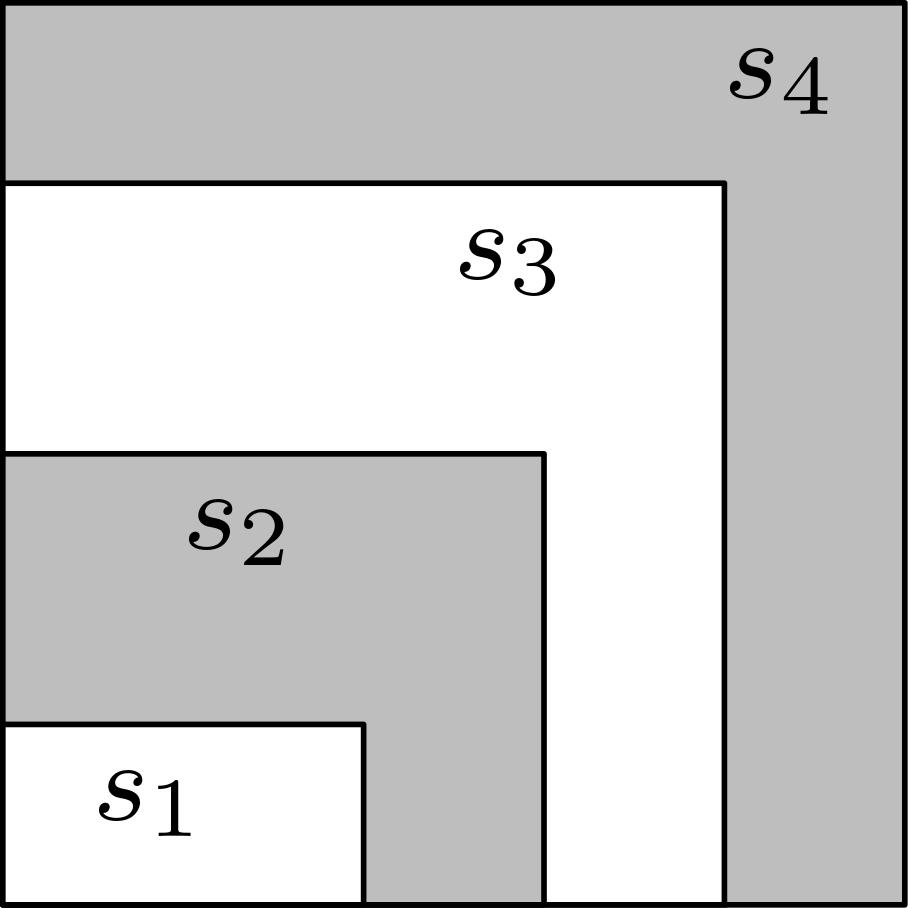
\includegraphics[width = 0.4\textwidth]{theory/area.png}
    \caption{Example for computing the area of overlapping polygons with areas $\text{Area}_{s_1} = 2$, $\text{Area}_{s_2} = 3$, $\text{Area}_{s_3} = 4$, $\text{Area}_{s_4} = 5$. It is incorrect to compute $\text{Area}_{s_1 + s_3} = 2 + 4 = 6$. Instead, $\text{Area}_{s_1 + s_3} = \text{Area}_{s_1 + s_2 + s_3 + s_4} - \text{Area}_{s_4} + \text{Area}_{s_3} - \text{Area}_{s_2} + \text{Area}_{s_1} = 5 - 5 + 4 - 3 + 2 = 3$.}
    \label{fig:areas}
\end{figure}

Similarly to Figure \ref{fig:areas}, we can compute the area seen exclusively by $g$. From the total area $\text{Area}_{\triangle_1 + \triangle_2, ..., \triangle_m}$ seen by $g$ we need to alternatively subtract the shared areas $\text{Area}_{\triangle_m}, ..., \text{Area}_{\triangle_4}, \text{Area}_{\triangle_2}$, then add the exclusively seen areas $\text{Area}_{\triangle_{m - 1}}, ..., \text{Area}_{\triangle_3}, \text{Area}_{\triangle_1}$.

% Figure \ref{fig:general_gradient} displays an example
% For each area seen by multiple guards, we know the length of the subsegments in between reflex vertex $r$ and the shared area beginning and ending, respectively. 
% In order to do so, we need to subtract the area $b_{i + 1}^2$ in between reflex vertex $r$ and the ending of the area, and then add back the area $b_i^2$ between $r$ and the beginning of the area. We need to repeat this process for each of the areas that are shared, in the direction starting from the polygon boundary to the reflex vertex.

This results in the fact that the area seen by $g$ exclusively can be computed as 
\begin{align*}
    \text{Area}_{\triangle_1 + \triangle_3 + ... + \triangle_{m - 1}} &= \text{Area}_{\triangle_1 + \triangle_2, ..., \triangle_m} - \text{Area}_{\triangle_{m - 1}} + \text{Area}_{\triangle_{m - 2}} - ... - \text{Area}_{\triangle_2} + \text{Area}_{\triangle_1} \\
                                                                      &= \left(b^2 - b_{m1}^2 + b_{(m - 1)2}^2 - ... - b_{12}^2 + b_{11}^2\right)\frac{\partial y}{2a}.
\end{align*}

Alternatively, if $\triangle_1$ is first seen by other guards (so $b_{11} = 0$), then all the signs are flipped. This claim can also be supported by the intuition of Figure \ref{fig:areas}. If we are interested in the areas of $s_2$ and $s_4$, then it is incorrect to compute them as $\text{Area}_{s_2 + s_4} = 3 + 5 = 8$. This is because $s_1$ and $s_3$ are overlapping in between them.  Instead, $\text{Area}_{s_2 + s_4} = \text{Area}_{s_1 + s_2 + s_3 + s_4} + \text{Area}_{s_4} - \text{Area}_{s_3} + \text{Area}_{s_2} - \text{Area}_{s_1} = 5 + 5 - 4 + 3 - 2 = 7$.

\subsection{Momentum}

In this section we introduce an improvement to the regular gradient descent algorithm: momentum. Its aim is to smoothen out the large noisy jumps in the gradient descent computation \cite{goodfelow2016deep}. Momentum builds upon the idea of considering the past states of the gradient descent computation. In this way, the past states create ``inertia'' to the newly computed gradient state. This results in the overall optimisation trajectory to be smoother.

So, the position $g_i$ at iteration $i$ of a guard $g$ will not be calculated anymore based only on the current computation of gradient descent. Instead, it will also take into account past values of gradient descent. In order to decide how much past states influence the value of the current position, we will take each gradient value with a weight.

Let $M_i$ be the momentum for a guard per iteration $i$. Let $\Delta f_i$ be the computation of the gradient descent in iteration $i$. Let the weight of a gradient descent value be a hyperparameter $\gamma$. 
As such, we can take into account the value of the previous gradient $\Delta_{i - 1}$ with weight $\gamma$. However, we still want the current gradient $\Delta f_i$ to influence the guard's movement. This can happen with a weight of $1 - \gamma$. So, the computation for the momentum at iteration $i$ becomes $$M_i = \gamma M_{i - 1} + (1 - \gamma)\Delta f_i.$$

Let $$M_0 = (1 - \gamma) \Delta f_0.$$. We can then check for correctness how  the next iterations of the momentum are carried out:
\begin{align*}
    M_1 &= \gamma M_0 + (1 - \gamma) \Delta f_1 \\
        &= \gamma (1 - \gamma) \Delta f_0 + (1 - \gamma) \Delta f_1 \\
        &= (1 - \gamma) (\gamma \Delta f_0 + \Delta f_1) \\
    M_2 &= \gamma M_1 + (1 - \gamma) \Delta f_2 \\
        &= \gamma (1 - \gamma) (\gamma \Delta f_0 + \Delta f_1) + (1 - \gamma) \Delta f_2 \\
        &= (1 - \gamma) (\gamma^2 \Delta f_0 + \gamma \Delta f_1 + \Delta f_2) \\
    ... \\
    M_i &= \gamma M_{i - 1} + (1 - \gamma) \Delta f_i \\
        &= (1 - \gamma) (\gamma^i \Delta f_0 + \gamma^{i - 1} \Delta f_1 + ... + \gamma \Delta f_{i - 1} + \Delta f_i) \\
\end{align*}

In this way, our momentum computation exponentially decreases the influence of a past state over the guard's current movement. So, the previous value of the momentum will exert its inertia with $\gamma$ influence over the new value of the momentum.

Similarly, the new position $g_i$ of guard $g$ will now be calculated as $$g_i = g_{i - 1} + \alpha M_i.$$

\subsection{Reflex Vertex Pull}

In this section we introduce an additional improvement to our gradient descent algorithm with momentum: pulling a guard towards reflex vertices. The pull strategy makes use of the second derivative of our optimisation function $f(g) = \text{Area}(g)$.

% The first derivative primarily tells us about the direction the function is going. That is, it tells us if the function is increasing or decreasing.

% the second derivative tells us what the rate of change of a quantity is

As mentioned previously, we are using the first derivative to compute the gradient of a guard's movement. That is, we use the first derivative of $f$ to find the direction of a guard's movement that increases its seen area. Additionally, we can also make use of the second derivative of $f$ to explore what the rate of change of the area increase is. 

We can achieve a more rapid increase in the seen area if we move a guard closer to a reflex vertex. The closer a guard is moved to a reflex vertex, the larger the increase in the area seen past the vertex. If a guard is moved directly on a reflex vertex, then the area seen past the vertex is maximised. An example of the latter case can be seen in Figure \ref{fig:top_reflex_vertex}. There, the guard $g$ has been moved on top of reflex vertex $r$ such that it can see the whole area behind it.

\begin{figure}[h!]
    \centering
    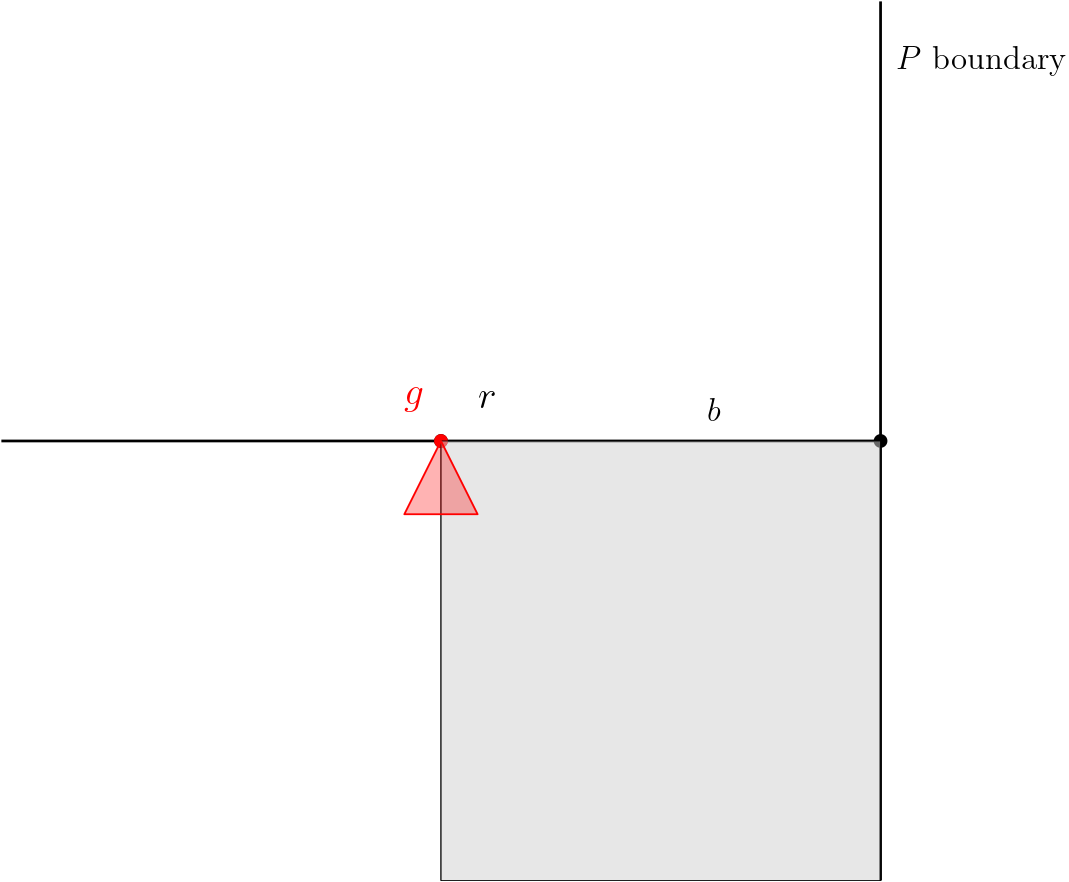
\includegraphics[width = 0.5\textwidth]{theory/pull2.png}
    \caption{Guard placed on top of a reflex vertex can now see the whole area behind the reflex vertex.}
    \label{fig:top_reflex_vertex}
\end{figure}

We will now explore how the pull towards a reflex vertex $r$ can be computed. Let $h_r$ be the pull in question, as shown in Figure \ref{fig:pull}. Let $g'_y$ be the new coordinates of guard $g$ when only the gradient is taken into account. In that case, we are only interested in the small movement $\partial y$. Analogously, let $g'_x$ be the new coordinate of guard $g$ when $g$ moves by a small amount $\partial x$ towards in the direction of the reflex vertex pull. As previously, and without losing generality, we are interested in a rotation of the plane $R$ such that $g$ and $r$ have the same $x$-coordinate. 

The pull is thus the second derivative of the gradient, so $$h_r = \bigtriangledown (\bigtriangledown f_r) = \left(\frac{\partial \bigtriangledown f}{\partial x}, \frac{\partial \bigtriangledown f}{\partial y}\right)^\intercal = \left(\frac{\partial \bigtriangledown f}{\partial x}, 0\right)^\intercal.$$  We can now calculate $h_r$ as follows: the norm of the gradient is $||\bigtriangledown f|| = \frac{b^2}{2a}$, so the norm of the second gradient as 
\begin{align*}
||h_r||&= ||\bigtriangledown (\bigtriangledown f)|| \\
       &= \bigtriangledown (\frac{b^2}{2a}) \\
       &= \frac{b^2}{2a}\frac{d}{da} \\
       &= b^2\frac{1}{2a}\frac{d}{da} \\
||h_r||&= -b^2\frac{1}{2a^2}.
\end{align*}

\begin{figure*}[!h]
    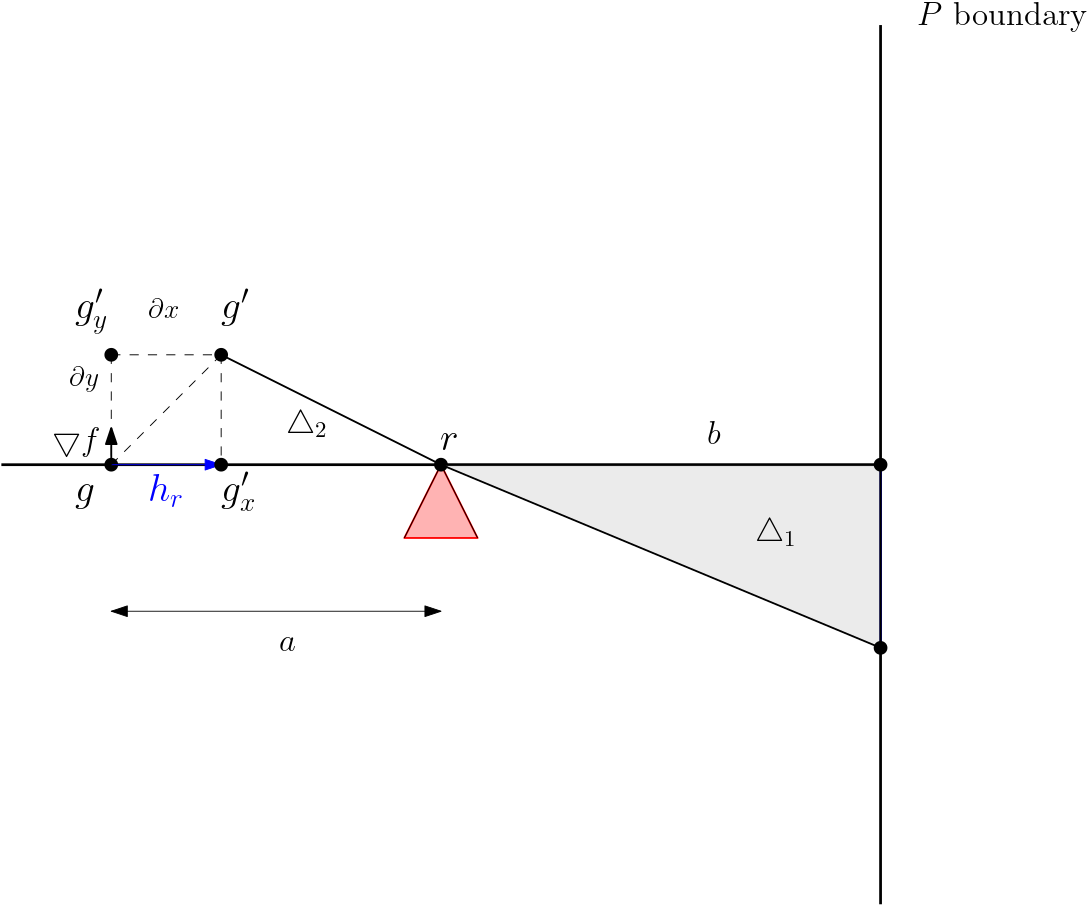
\includegraphics[width = 0.7\textwidth]{theory/pull.png}
    \centering
    \caption{Computing the movements of the guard based on both the gradient and the pull towards a reflex vertex. When only taking the reflex vertex pull into account, $g$ would need to move to $g'_x$. Similarly for when taking only the gradient into account, $g$ would need to move to $g'_y$. Combining the two movements together results in $g'$ being the final position of $g$.}
    \label{fig:pull}
\end{figure*}

The pull $h_r$ has the direction towards the reflex vertex $r$. So, it has the same orientation as vector $\vec{v} = (x, y)^\intercal$  from Figure \ref{fig:vperp}. We will normalise $h_r$ with the norm of vector $\vec{v}$. Its norm is $||\vec{v}|| = \frac 1 a$. So, $$h_r = \vec{v}\frac{-b^2}{2a^2}\frac 1 a = \vec{v}\frac{-b^2}{2a^3}.$$

Let $h$ be the total pull for guard $g$. As for the gradient, the total pull for guard $g$ and all reflex vertices $r$ the guard can see is $$h = \sum_{r \in R(g)} h_r, R(g) = \{\text{reflex vertices of $P$ seen by $g$\}}.$$

Therefore, the movement of a guard $g$ to the new position $g'$ will take both the gradient and the pull into account: $$g' = g + \alpha (\bigtriangledown f + h).$$ Additionally, we can choose how much influence the pull itself can have in the movement of the guard by adding a hyperparameter $\beta$: $$g' = g + \alpha (\bigtriangledown f + \beta h).$$

\subsubsection{Pull onto the Reflex Vertex}
We have now created a heuristic for pulling a guard closer to a reflex vertex based on the increase in the seen area behind the reflex vertex. It could happen however that the pull towards the reflex vertex is very strong. In this case, the guard could be moved past the reflex vertex, in between the reflex vertex and the polygon boundary. Although the area seen behind the reflex vertex would be maximised, the guard would ``unsee'' (parts of) the area of its initial position $g$. In order to address this particular issue, the guard will be placed on the reflex vertex when the pull is strong enough. 

This section will thus expand on a procedure that decides when a guard is best placed on a reflex vertex based on its pull towards it.

Firstly, we must define the condition of what a ``strong enough'' pull means. Such a pull would move the guard $g$ ``close enough'' to the reflex vertex. Hence, we need to compute what the upper limit of the distance between the new guard position $g'$ and reflex vertex $r$ would be. The most straight-forward way to do so would be to assign a hyperparameter to the distance between $g$ and $r$. Recall that $||\overline{gr}|| = a$. For now, let $\frac 2 3$ be the factor of closeness of $g'$ to $r$. This means, that when the pull is stronger than $\frac 2 3$ times the distance $a$, then the guard is moved onto the reflex vertex: $$h_r > \frac 2 3 a.$$


\begin{figure}[h!]
    \centering
    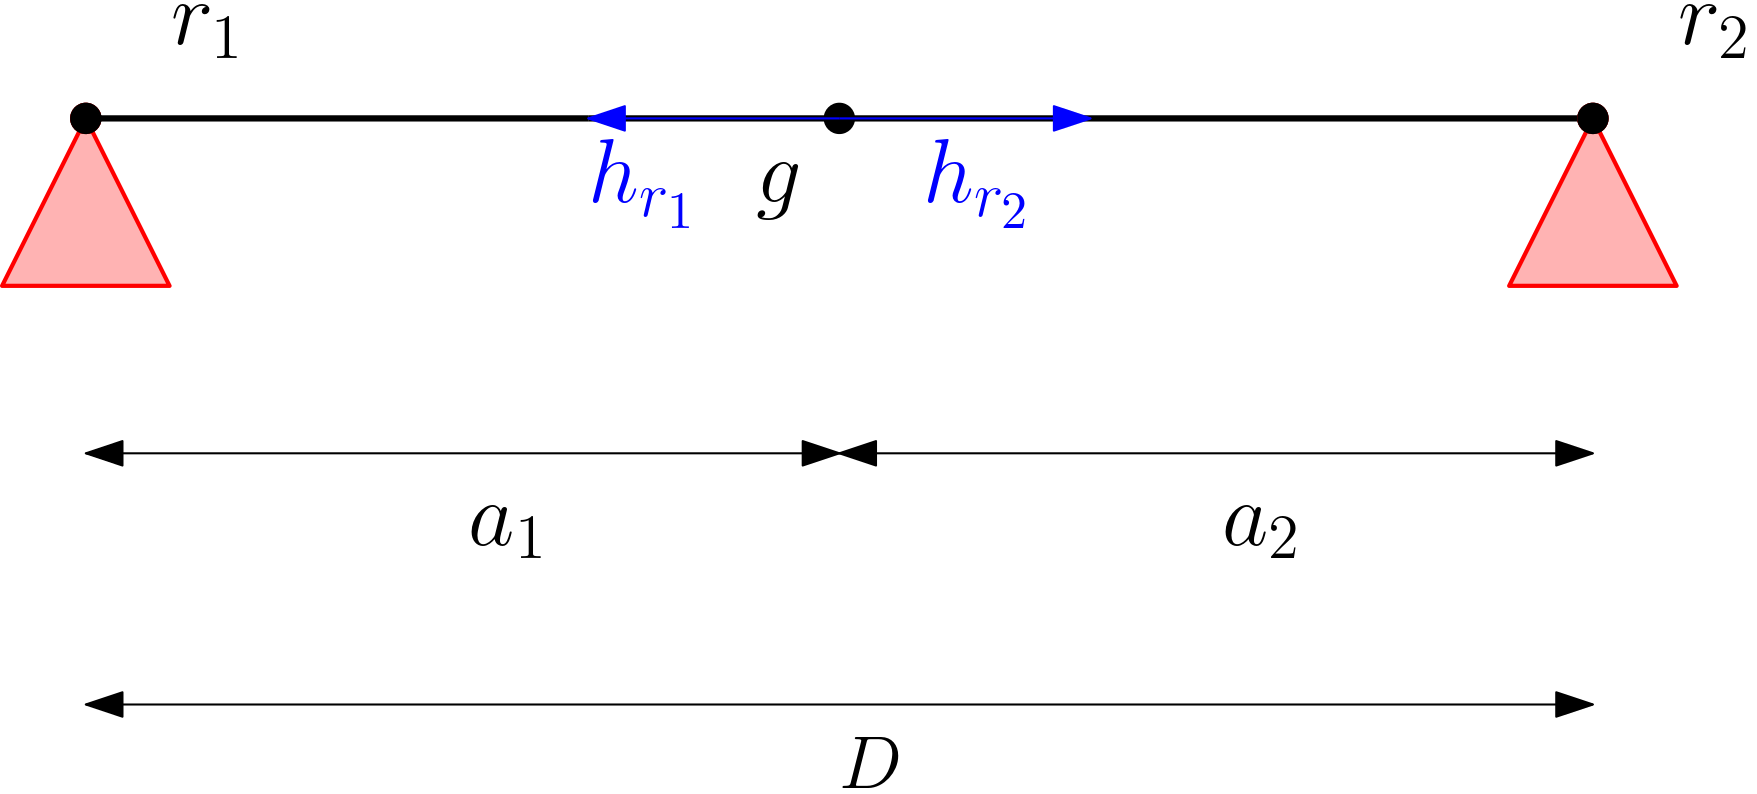
\includegraphics[width = 0.5\textwidth]{theory/pull3.png}
    \caption{Guard $g$ is in between two reflex vertices $r_1$ and $r_2$. Because they are collinear and $g$ is equidistant from them, the two pulls $h_{r_1}$ and $h_{r_2}$ cancel each other out.}
    \label{fig:pull_cancel}
\end{figure}

Next, we need to account for the case where a polygon has multiple reflex vertices. Namely, we consider the specific edge case when a guard is in between two reflex vertices, illustrated in Figure \ref{fig:pull_cancel}. Thus, let $r_1$ and $r_2$ be two reflex vertices whose distance $$D = \min_{q \neq r} \text{ distance}(q, r), \forall q, r \in P \text{ reflex vertices}.$$
Let $g$ be a guard in between $r_1$ and $r_2$. Let the pulls $h_{r_1}$ and $h_{r_2}$ be  individually strong towards $r_1$ and $r_2$, respectively. However, because they are opposites in directions, they cancel each other out, resulting in $g$ possibly not changing its position at all.

We will now introduce another condition for pulling the guard towards the closer reflex vertex when pulls are cancelling each other out. If a guard $g$ is not equidistantly placed in between two reflex vertices, we are interested in computing what the closer reflex vertex is. So, if $g$ is closer than $\frac D 2$ to a reflex vertex, then we consider it close enough if: $$a < \frac D 2.$$
In this case we can choose to still move towards one of the reflex vertices and make progress.



\subsection{Reflex Area}
% - address the issue of a guard "losing" the seen area gained after moving on top of a reflex vertex + its movement in and out of the reflex vertex
In this section we introduce an additional extension to the gradient descent algorithm with momentum and reflex vertex pull: the concept of a reflex area. 

The Reflex Area design choice was made to counter-act the edge case of a guard moving away from a reflex vertex and ``unseeing'' the area that it was already seeing. This case is illustrated in Figure \ref{fig:pull_to_on_behind}. In Subfigure \ref{fig:pull_to_on_behind1}, guard $g$ starts moving with pull $h_r$ towards reflex vertex $r$. The pull is strong enough to place $g$ on $r$ in Subfigure \ref{fig:pull_to_on_behind2}. In this case, $g$ can see everywhere around $r$. However, the new gradient $\bigtriangledown f$ of $g$ moves it past $r$ in Subfigure \ref{fig:pull_to_on_behind3}. The initially seen area before $r$ is now not completely seen anymore by $g$.

\begin{figure}[h!]
    \centering
    \begin{subfigure}{0.45\textwidth}
        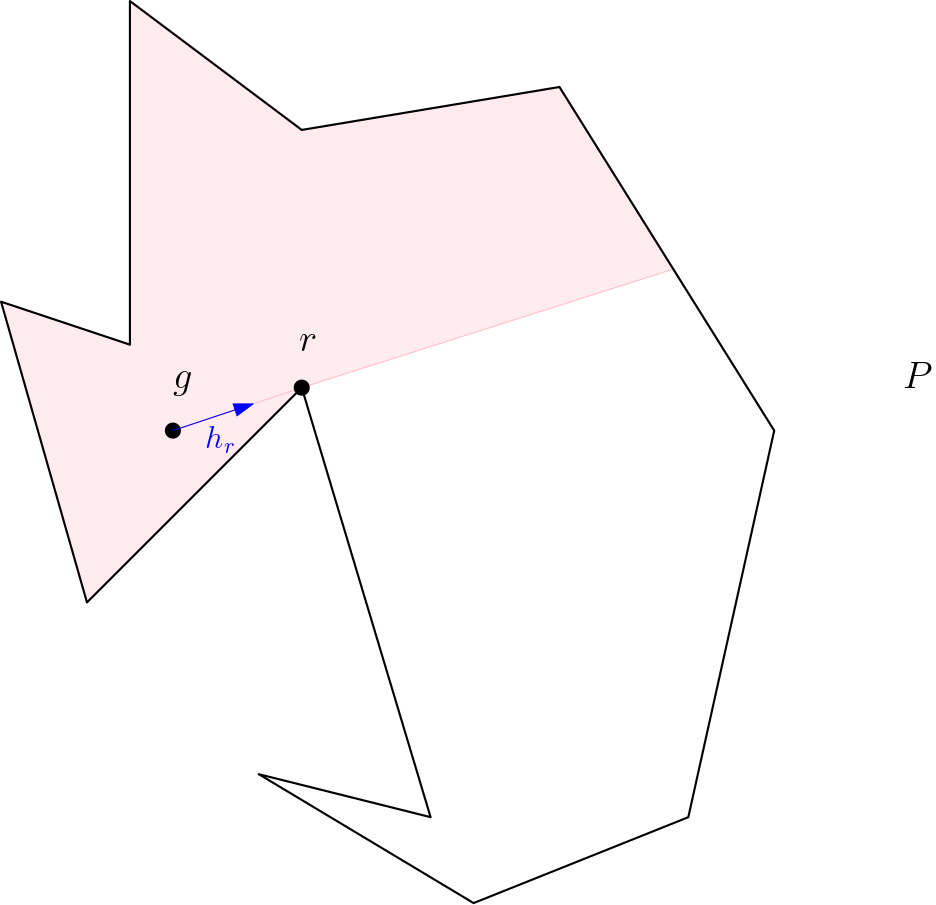
\includegraphics[width = \textwidth]{theory/reflex_area_to_vertex.png}
        \caption{Guard $g$ starts moving with pull $h_r$ towards reflex vertex $r$. Guard $g$ cannot see past $r$.}
        \label{fig:pull_to_on_behind1}
    \end{subfigure}
    \hfill
    \begin{subfigure}{0.45\textwidth}
        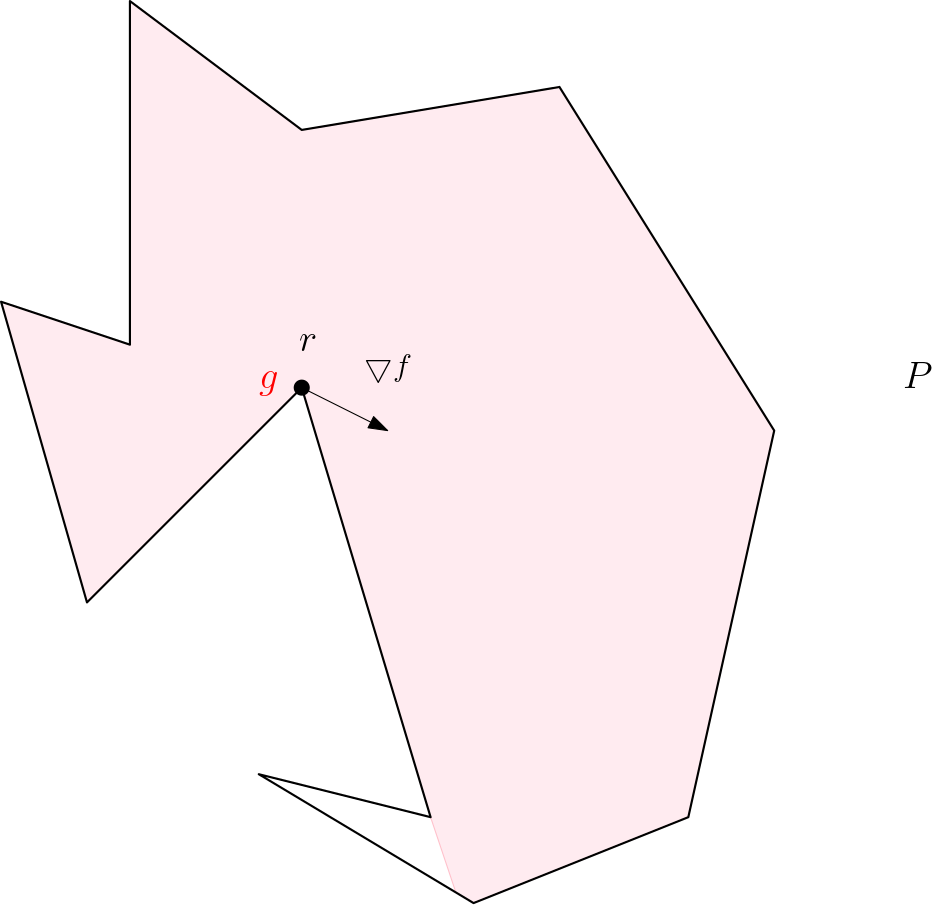
\includegraphics[width = \textwidth]{theory/reflex_area_on_vertex.png}
        \caption{Guard $g$ is placed on reflex vertex $r$. Guard $g$ can see both before $r$ and past it.}
        \label{fig:pull_to_on_behind2}
    \end{subfigure}
    \begin{subfigure}{0.6\textwidth}
        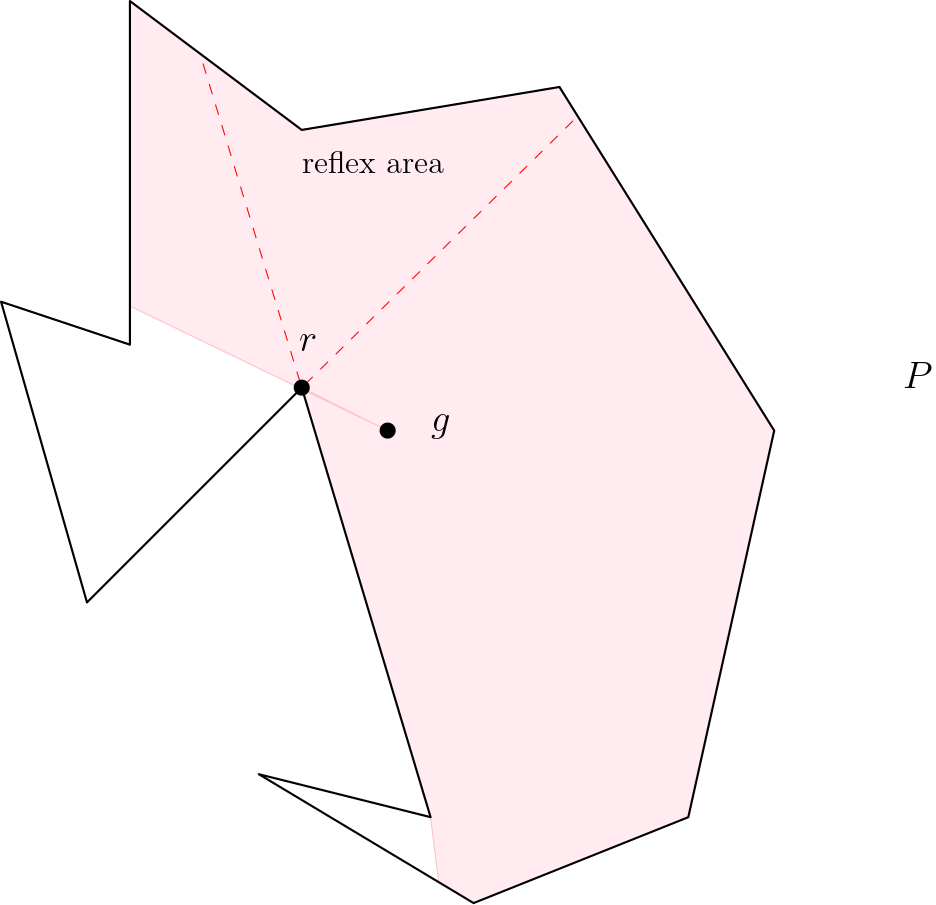
\includegraphics[width = \textwidth]{theory/reflex_area_behind_vertex.png}
        \caption{Guard $g$ has moved past reflex vertex $r$. Guard $g$ cannot see anymore before $r$.}
        \label{fig:pull_to_on_behind3}
    \end{subfigure}
    \caption{Guard $g$ moves towards and on the reflex vertex $r$. Eventually, its newly computed position is away from $r$ and the reflex area. This results in $g$ not seeing the initial area anymore.}
    \label{fig:pull_to_on_behind}
\end{figure}


Let $rr'$ and $rr''$ be the extensions to the polygon boundary segments whose intersection is the reflex vertex $r$. We call \textit{reflex area} the area between lines $rr'$ and $rr''$ that is contained inside the polygon. Figure \ref{fig:reflex_area} draws this concept. If a guard $g$ has to move outside of the reflex area, we project its new position onto the closest reflex line (in this case, $rr'$) as $g'$. Naturally, if $g$ has to move inside the reflex area, it can do so unalteredly. In this way, we maintain the gained property of a guard seeing everything around a reflex vertex while still allowing it to move away from the reflex vertex.

\begin{figure}[h!]
    \centering
    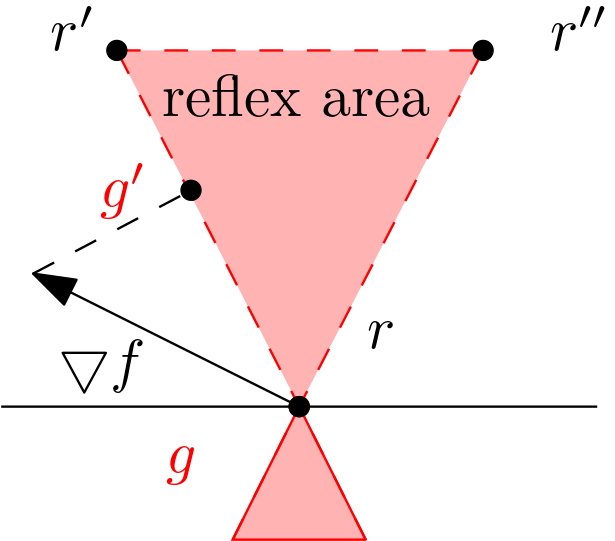
\includegraphics[width = 0.7\textwidth]{theory/reflex_area.png}
    \caption{Guard $g$ has been placed on the reflex vertex $r$. Hence, its movement is restricted to the reflex area created by the two reflex lines $rr'$ and $rr''$. So, if $g$ needs to move outside of the reflex area, its new position will be projected on the closest reflex line.}
    \label{fig:reflex_area}
\end{figure}


\subsection{Hidden Gradient}
% - speed up the guard movement by giving all guards a gradient
In this section we will introduce a computation speedup for the case in which guards have a gradient of 0 (they don't move). This can happen when the area seen by a guard is already seen by other guards too. We consider that having a gradient of 0 is detrimental to the progress of the algorithm. The reason behind this is that it is unlikely that a guard's optimal position has been found when its gradient is 0. Hence, we would like every guard to move, no matter how little.

In order to allow guards to still move when their gradient is 0, we deployed the Hidden Gradient heuristic. This heuristic is based on the fact that we allow guards whose gradient is 0 to still move with a newly computed ``hidden'' gradient. So, if there are guards whose gradient is 0, we will recompute their gradient by not taking into account the area seen by the guards who have a non-zero gradient.

An example of this approach can be found in Figure \ref{fig:hidden_gradient}. Let $G = \{g_1, g_2, g_3\}$ be the complete set of guards. Initially in Subfigure \ref{fig:hidden_gradient1}, only $g_1$ has a non-zero gradient. The visibility regions of $g_2$ and $g_3$ are overlapping with that of $g_1$, so their gradients are 0. Let $G_0 = \{g_1\}$ be the set of guards who at step 0 have a non-zero gradient. 
Then, Subfigure \ref{fig:hidden_gradient2} contains the set $G \setminus G_0$ of guards. The visibility area of guard $g_1$ overlaps with $g_2$, so only guard $g_2$ will have a non-zero gradient. Let $G_1 = \{g_2\}$ be the set of guards who at step 1 have a non-zero gradient.
Lastly, we can compute the non-zero gradient for guard $g_3$ in Subfigure \ref{fig:hidden_gradient3}. Let $G_2 = \{g_3\}$ be the set of guards who at step 2 have a non-zero gradient.
In Subfigure \ref{fig:hidden_gradient4} all the guards have been moved to their new positions $g'_1, g'_2, g'_3$, respectively. So the gradients have been computed as $G = G_0 \cup G_1 \cup G_2$, where $G_1$ and $G_2$ contain the guards with hidden gradients.

\begin{figure}[h!]
    \centering
    \begin{subfigure}{0.45\textwidth}
        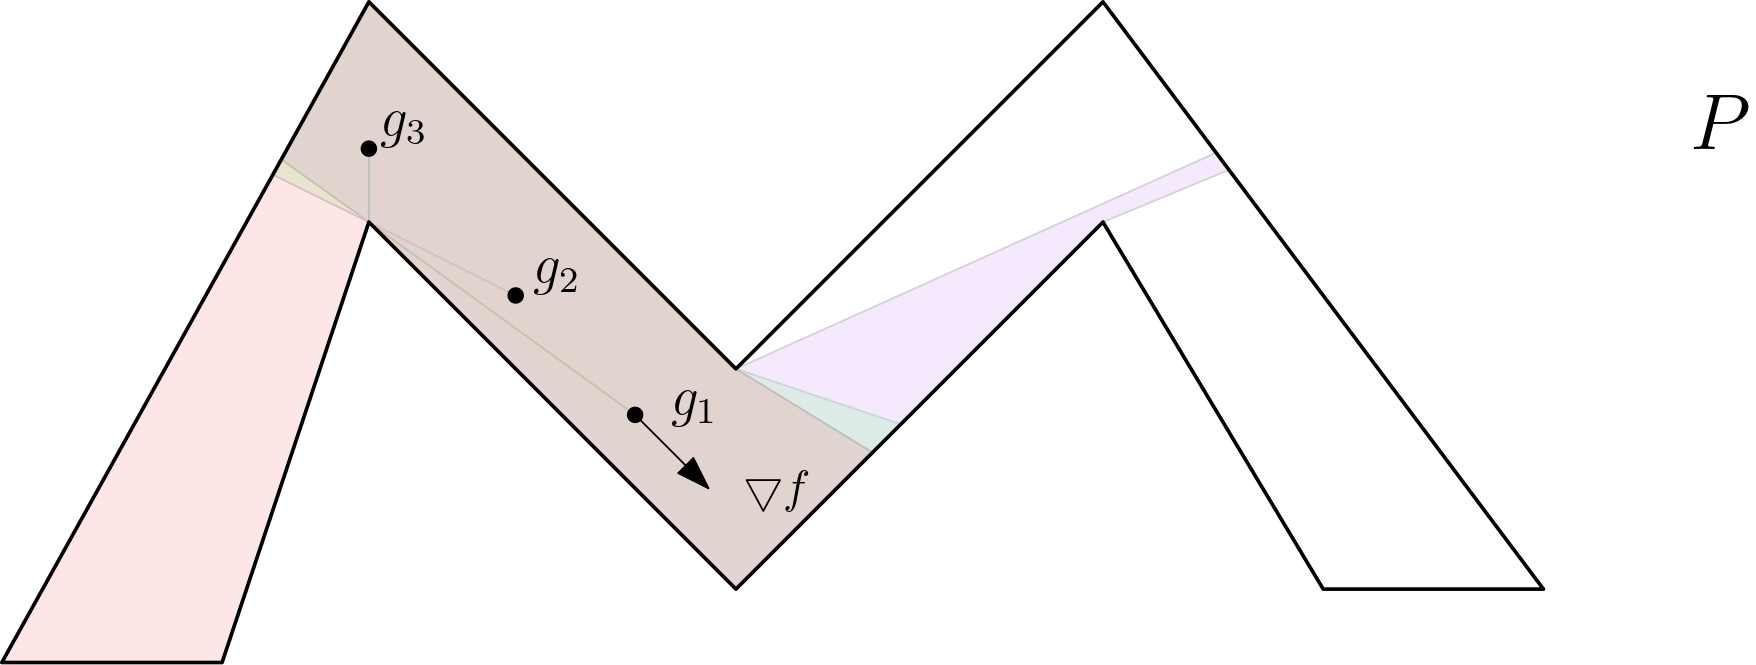
\includegraphics[width = \textwidth]{theory/hidden_gradient1.png}
        \caption{Guard $g_2$ and $g_3$ have a gradient of 0, because guard $g_1$ sees all the areas they see. So, the set of guards with a non-zero gradient is $G_0 = \{g_1\}$.}
        \label{fig:hidden_gradient1}
    \end{subfigure}
    \hfill
    \begin{subfigure}{0.45\textwidth}
        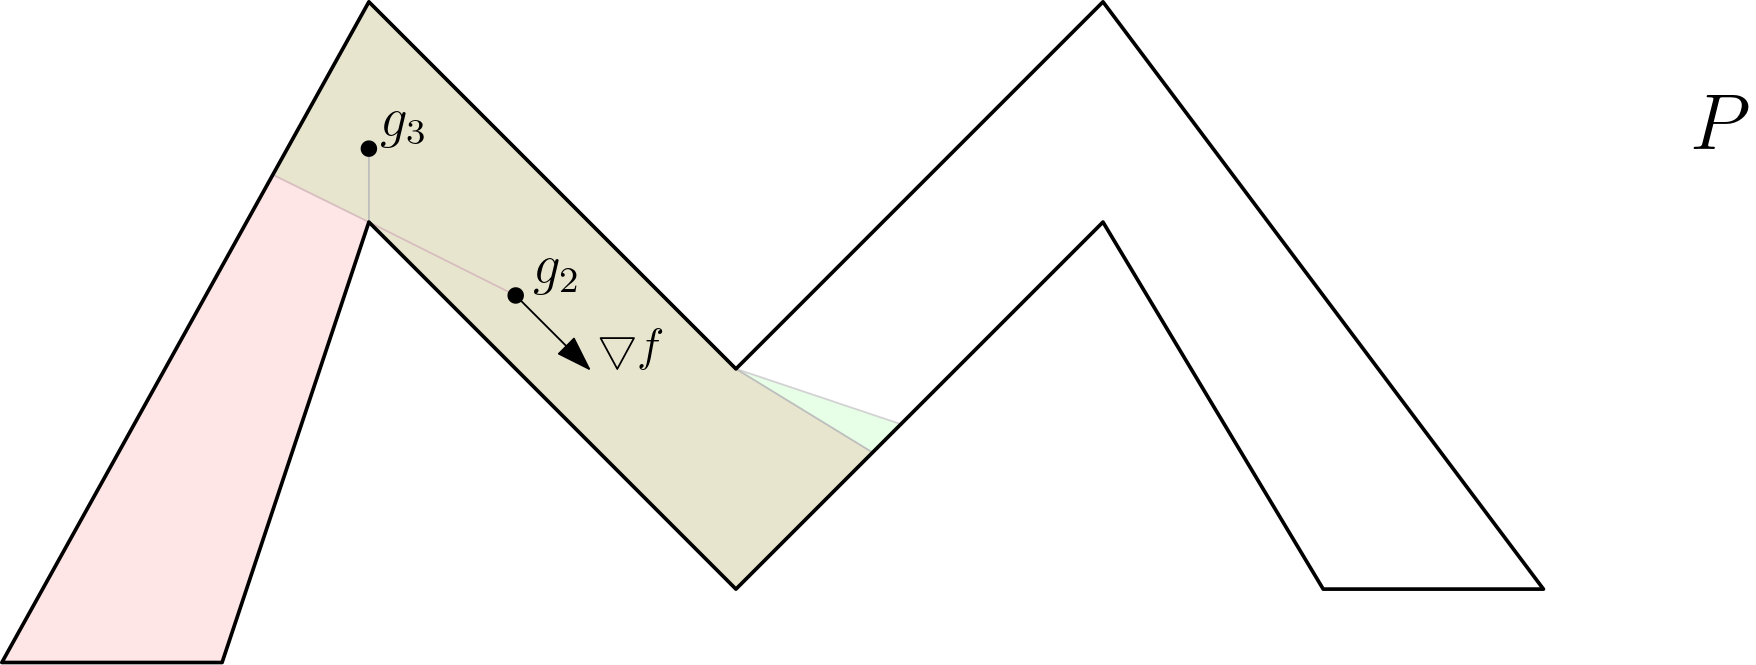
\includegraphics[width = \textwidth]{theory/hidden_gradient2.png}
        \caption{Guard $g_1$ had a non-zero gradient, so we compute the gradients of guards $g_2$ and $g_3$ without $g_1$. Guard $g_2$ sees everything that $g_3$ sees, so $g_3$ will have gradient 0. So, the set of guards with a non-zero gradient is $G_1 = \{g_2\}$.}
        \label{fig:hidden_gradient2}
    \end{subfigure}
    \begin{subfigure}{0.45\textwidth}
        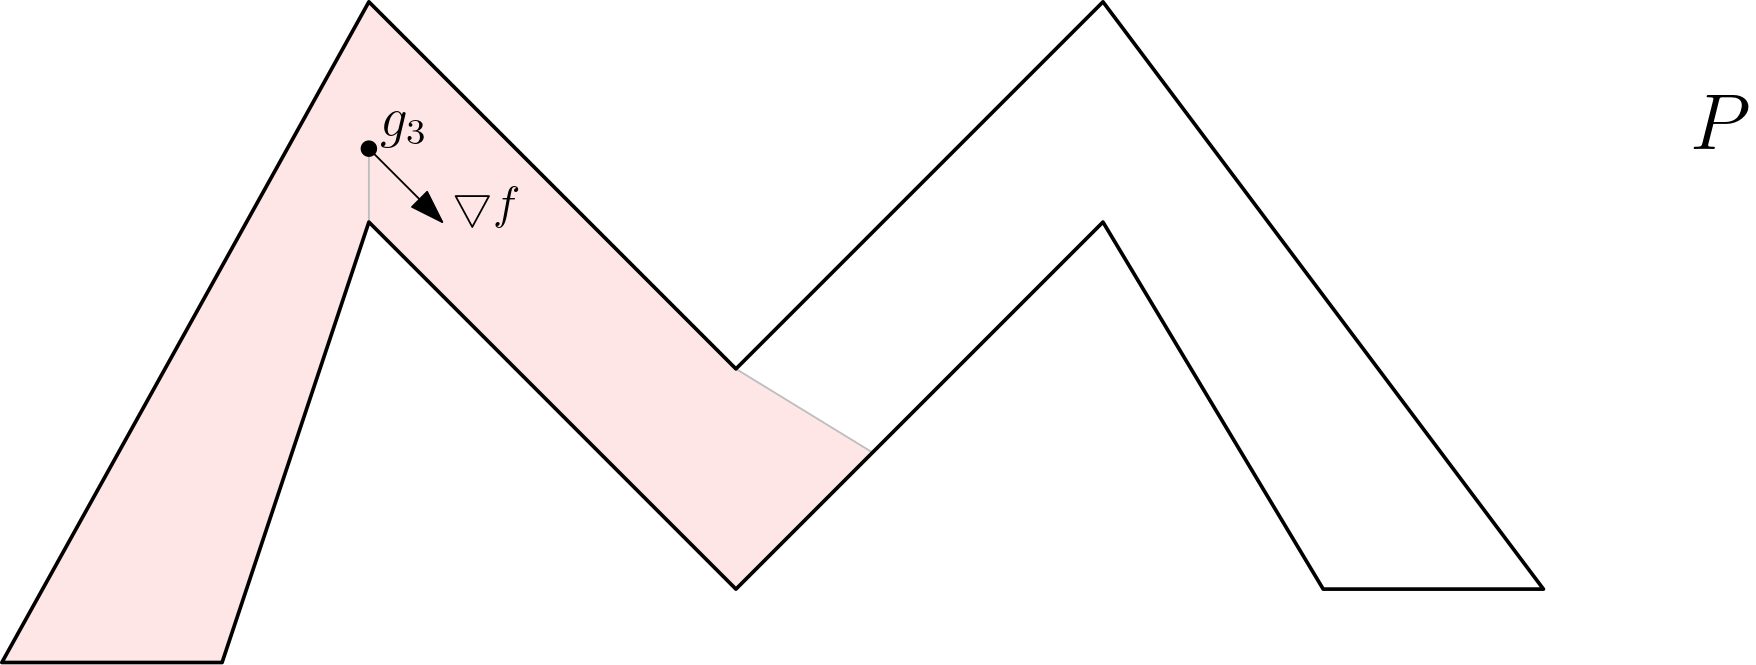
\includegraphics[width = \textwidth]{theory/hidden_gradient3.png}
        \caption{Guard $g_2$ had a non-zero gradient, so we compute the gradient of guard $g_3$ without $g_2$. Guard $g_3$ will now have a non-zero gradient. So, the set of guards with a non-zero gradient is $G_2 = \{g_3\}$.}
        \label{fig:hidden_gradient3}
    \end{subfigure}
    \hfill
    \begin{subfigure}{0.45\textwidth}
        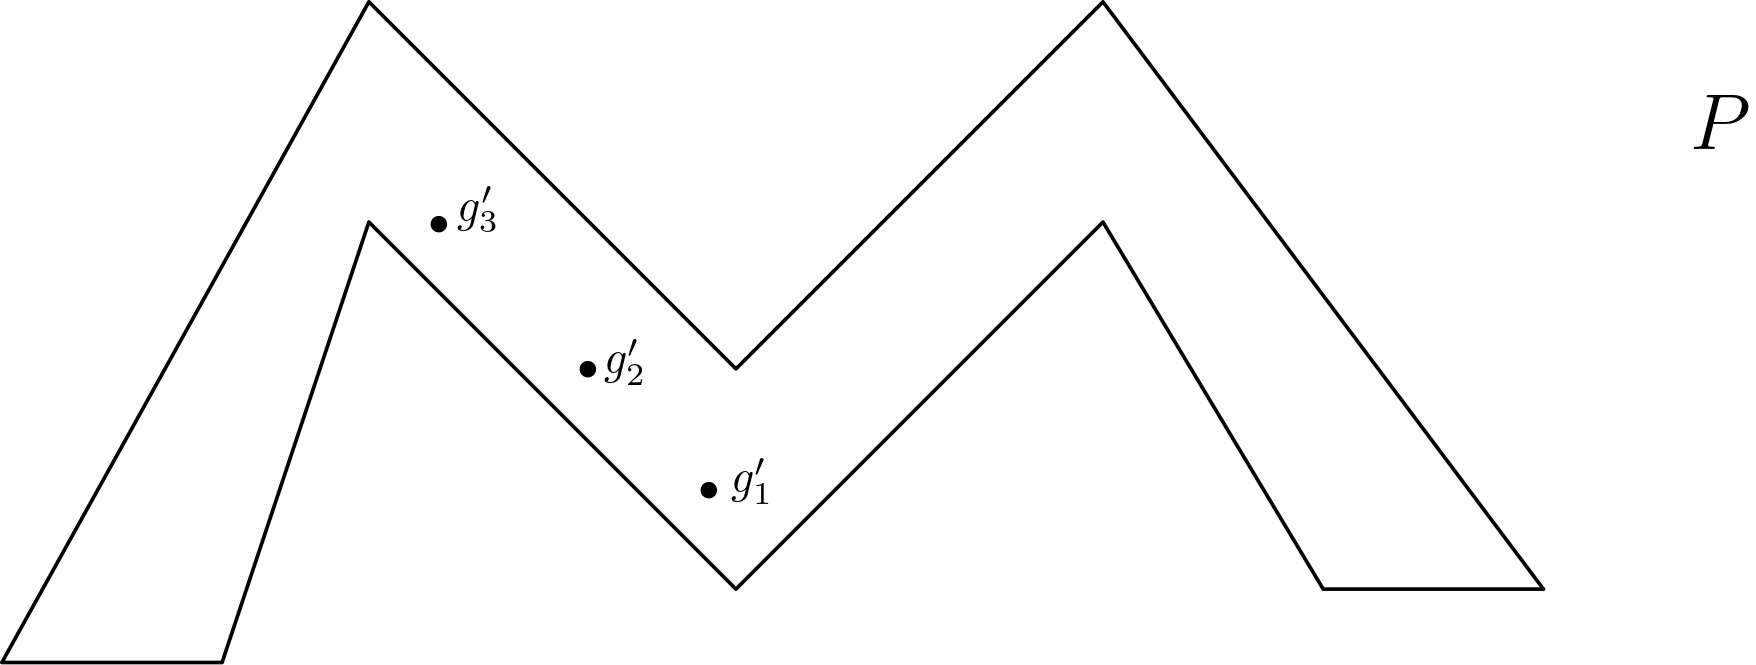
\includegraphics[width = \textwidth]{theory/hidden_gradient4.png}
        \caption{The new positions $g'_1, g'_2, g'_3$ of the guards such that $G = G_0 \cup G_1 \cup G_2$.}
        \label{fig:hidden_gradient4}
    \end{subfigure}
    \caption{Example of hidden gradient computation for guard set $G = \{g_1, g_2, g_3\}$ in a corridor-like polygon. The visibility areas of each of the guards $g_1, g_2$, and $g_3$ are shown in purple, green and orange, respectively.}
    \label{fig:hidden_gradient}
\end{figure}

The hidden gradient heuristic can now be generalised. Let $G$ be the complete set of guards. For each step $i$, let $G_i = G \setminus G_{i - 1}$ be the set of guards with a non-zero gradient after removing the guards with a gradient from step $i - 1$. The set $G_0$ will be the set of guards with a non-zero gradient before removal of any guards. At the end, the union of all subsets $G_i$ will comprise the set of all guards $G = G_0 \cup G_1 \cup ...$.
In this way, all guards will have a non-zero gradient and make progress.

\subsection{Greedy Initialisation}
% - head start
In this section we will introduce another heuristic for improving the performance of the gradient descent with momentum algorithm: Greedy Initialisation. This heuristic will give a head start to the algorithm by arbitrarily placing guards in areas that are unseen by other guards. In this way, the algorithm will start with an already much larger covered area.

Figure \ref{fig:greedy} offers an example of a Greedy Initialisation. The first guard $g_1$ is arbitrarily placed inside polygon $P$ as shown in Subfigure \ref{fig:greedy1}. Then, guard $g_2$ is arbitrarily placed in an unseen part of $P$, as displayed in Subfigure \ref{fig:greedy2}. In this way, the algorithm gains a head start to continue with the optimisation of the guards' positions.

\begin{figure}[h!]
    \centering
    \begin{subfigure}{0.45\textwidth}
        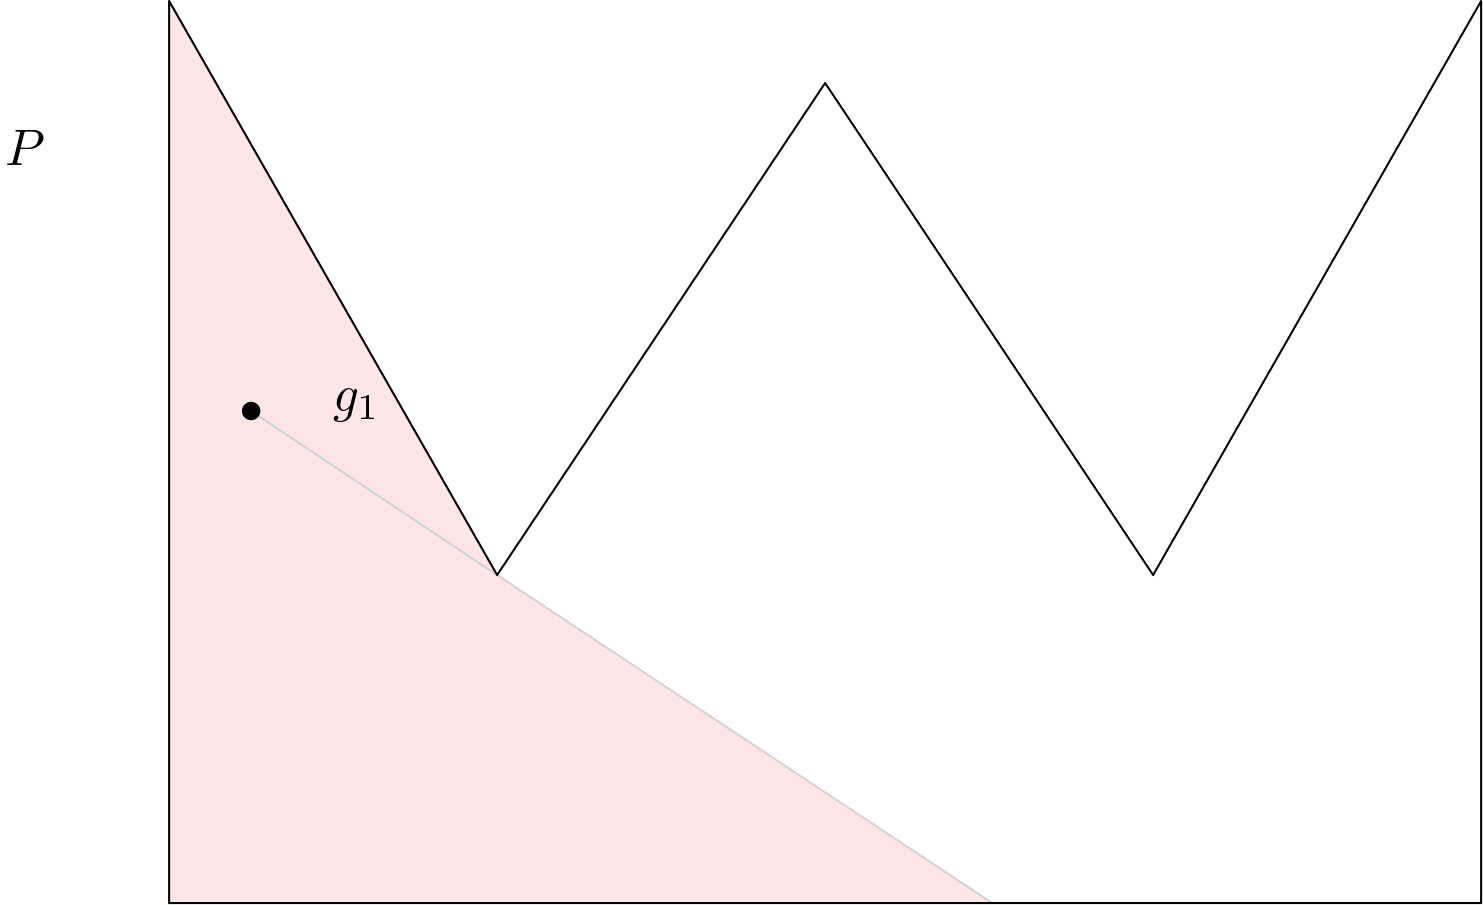
\includegraphics[width = \textwidth]{theory/greedy1.png}
        \caption{Guard $g_1$ has been arbitrarily placed inside the polygon $P$.}
        \label{fig:greedy1}
    \end{subfigure}
    \hfill
    \begin{subfigure}{0.45\textwidth}
        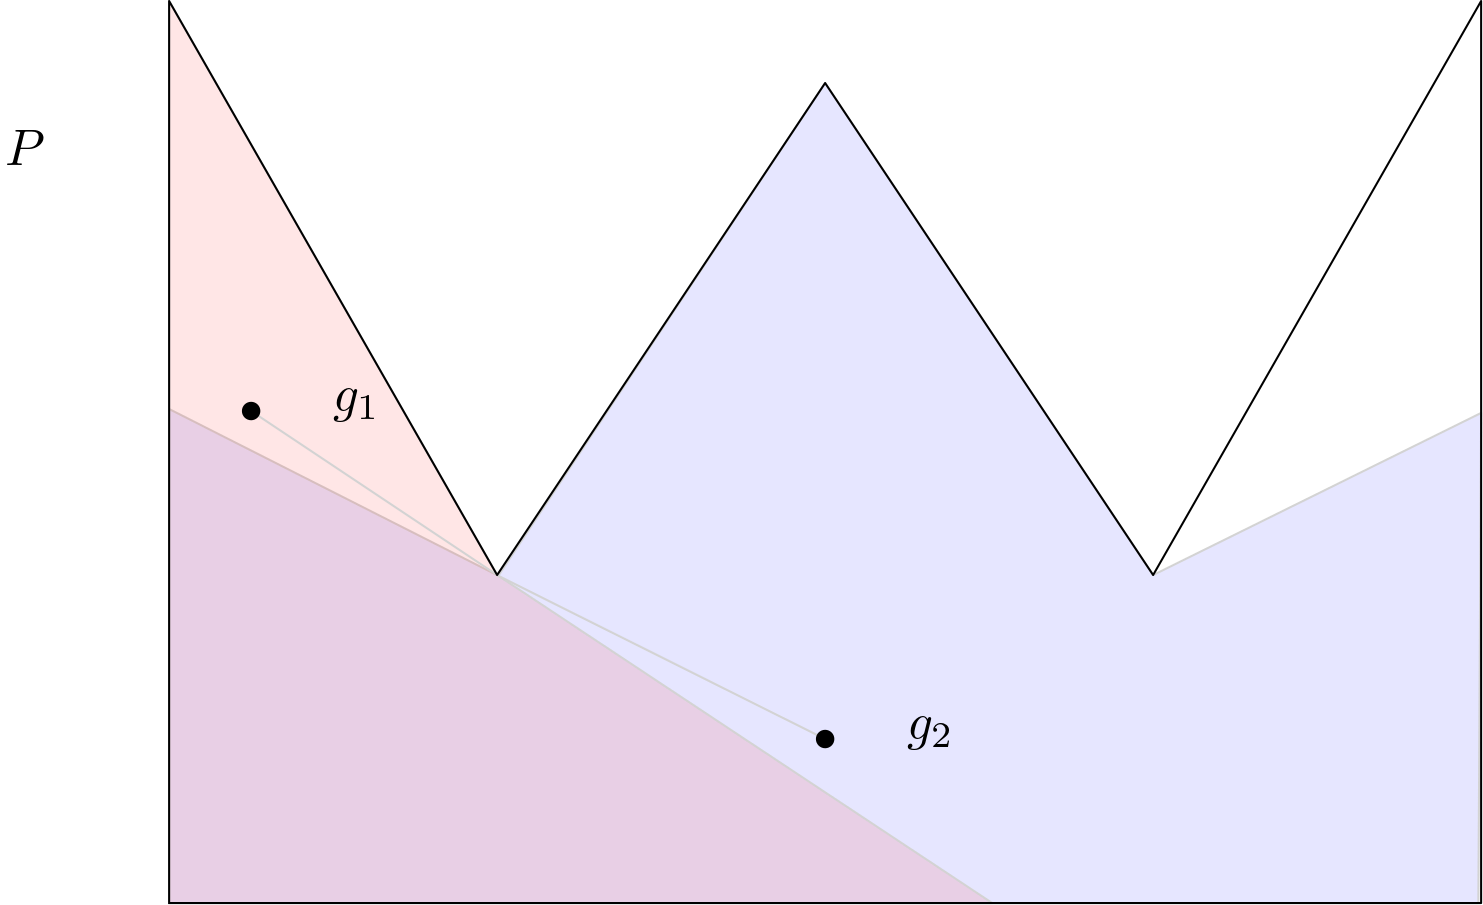
\includegraphics[width = \textwidth]{theory/greedy2.png}
        \caption{Guard $g_2$ has been arbitrarily placed inside the polygon $P$, outside of the visibility region of guard $g_1$.}
        \label{fig:greedy2}
    \end{subfigure}
    % \begin{subfigure}{0.45\textwidth}
    %     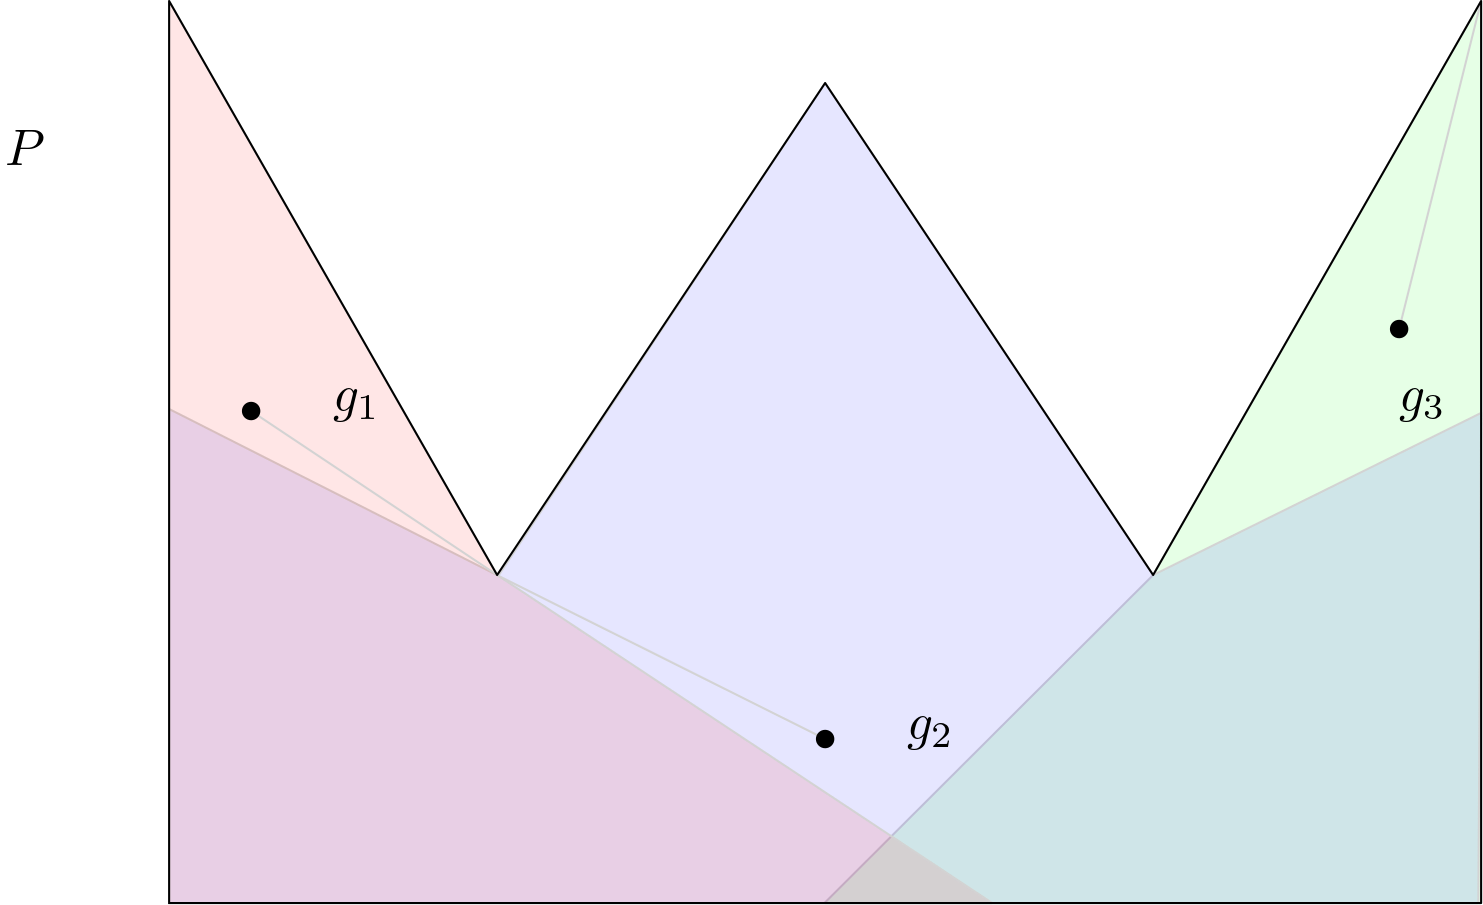
\includegraphics[width = \textwidth]{theory/greedy.png}
    %     \caption{Guard $g_3$ has been arbitrarily placed inside the polygon $P$, outside of the visibility regions of guards $g_1$ and $g_2$.}
    %     \label{fig:greedy3}
    % \end{subfigure}
    \caption{Greedy Initialisation for guards $g_1$ and $g_2$ inside polygon $P$. The visibility regions of the guards are displayed in orange and purple, respectively. In this way, the algorithm gains a head start for optimising the positions of the guards.}
    \label{fig:greedy}
\end{figure}

\subsection{Angle Behind Reflex Vertex}
% - take into consideration how much a guard should move towards a reflex vertex, depending on the area seen behind it
In this section we will introduce a heuristic that will further fine-tune the factor with which a guard is influenced by a reflex vertex. Currently, we only take into account the distance $b$ between the reflex vertex and the polygon boundary. Intuitively, the unseen area behind the reflex vertex should also play a role in the computation of the gradient: guards should be drawn faster to larger areas. In order to do so, we will take into account the normalised value of angle $\mu$ behind the reflex vertex.

A visualisation for this heuristic can be found in Figure \ref{fig:angle}. The pull of the guard $g$ towards the reflex vertex $r$ will be influenced by the normalised value of $\mu$ as follows: $$g' = g + \alpha \frac{\mu}{2\pi}(\bigtriangledown f + \beta h).$$

\begin{figure}[h!]
    \centering
    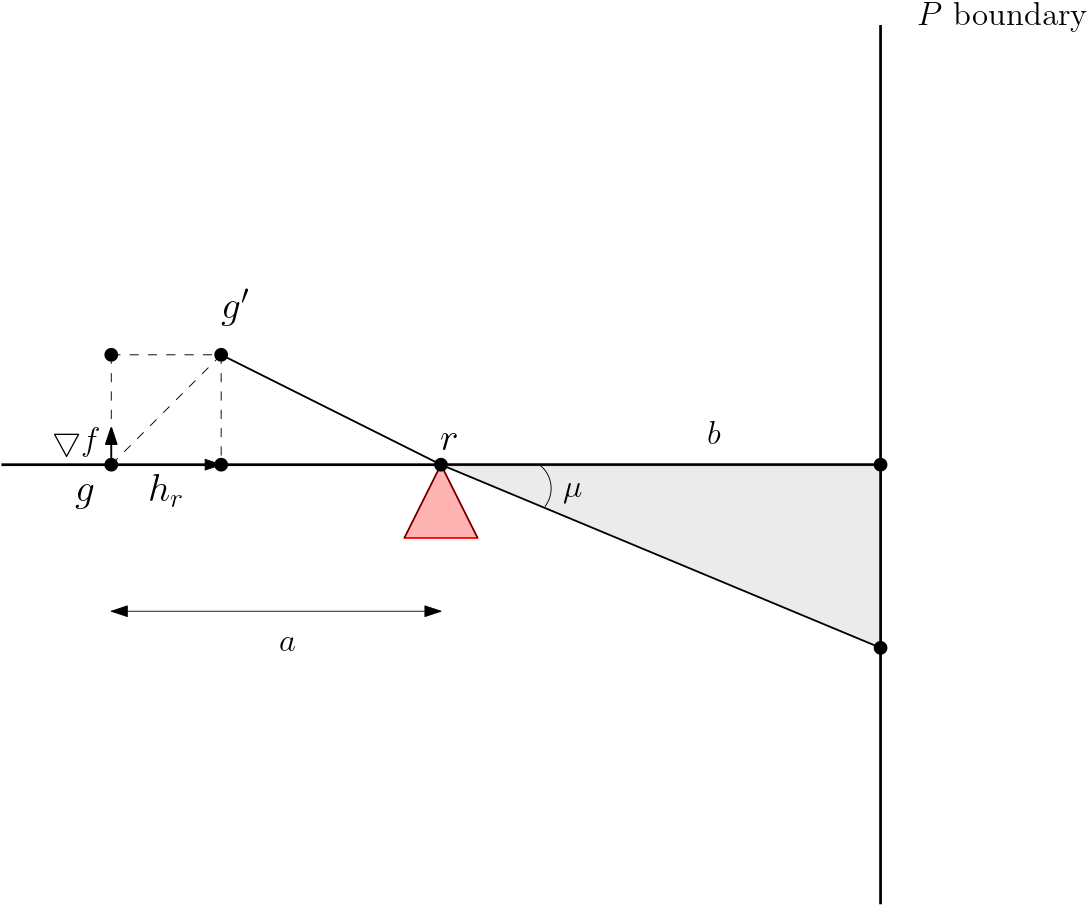
\includegraphics[width = 0.6\textwidth]{theory/angle.png}
    \caption{The normalised angle $\mu$ behind the reflex vertex $r$ takes into account the factor with which the guard $g$ is drawn to $r$.}
    \label{fig:angle}
\end{figure}
\section{Practice}
\label{sec:experiments}

This section will provide the implementation details of the theory part (Section \ref{sec:theory}). The algorithm is implemented in C ++ and makes use of the CGAL library (\url{https://www.cgal.org}). 
Then, given the implementation, experimental setups will be introduced. The experiments will include basic test polygons to showcase the execution of the algorithm. We will also observe the importance of each of the heuristics used. Lastly, we will observe how the algorithm scales in the context of the comb polygon.

% Polygons used:
% - 2 guards
% - random
% - love
% - comb
% - corridor

% For every heuristic:
% - show how each polygon behaves when turning it off

% Try to see if the comb polygon scales

\subsection{Heuristics}
In this subsection we will observe the role played by each of the heuristics used. We will additionally notice how different heuristics are relevant for different types of polygons. In order to do so, we will run the program with all the heuristics but one, for each of the heuristics. By analysing the difference in movement for each of the guards, we will be able to assess the influence every heuristic has on different types of polygons.

We will use fixed hyperparameters for all the runs. This will allow us to focus on the differences between the heuristics. 
% Later in this section we will also discuss the actual hyperparameter choice. 
As such, we will use the momentum hyperparameter $\gamma = 0.8$ and pull attraction $\beta = 1$. The hyperparameter values were chosen through experimentation. The algorithm is sensitive to the hyperparameter choices, so for other values it often becomes stuck in local optima.

\subsubsection{Without Momentum}
In this section we will discuss the impact momentum has on the overall behaviour of the algorithm. As introduced in Section \ref{sec:momentum}, momentum takes into account the position history of the guards. In this way, the overall trajectory of a guard is smoothened out.

A suggestive way to observe this is with the arbitrary polygon from Figure \ref{fig:random}. The polygon requires a minimum of 3 guards to be fully seen.

\begin{figure}[h!]
    \centering
    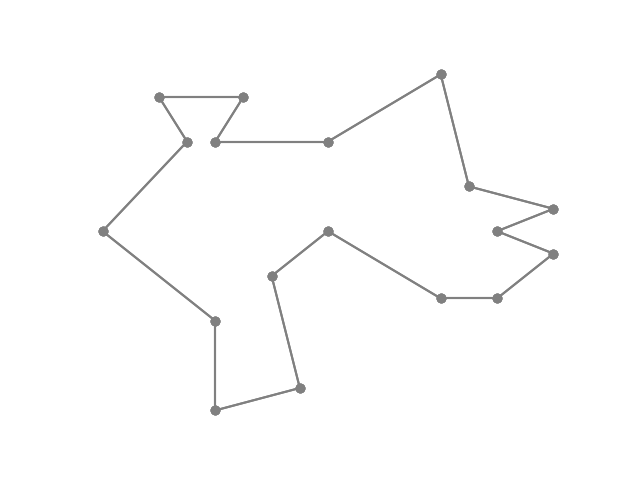
\includegraphics[width = 0.5\textwidth]{experiments/random.png}
    \caption{Arbitrarily shaped polygon.}
    \label{fig:random}
\end{figure}

We will compare how the guards move when we are using all the heuristics to when we are not using momentum. They will start at the same fixed position in both cases.

Figure \ref{fig:no_momentum} displays the area seen per iteration for the arbitrary polygon. Both the total and the individual areas seen by each guard are shown. Starting with almost the whole polygon seen, the guards are eventually optimally placed. Nonetheless, using momentum clearly makes a difference in Subfigure \ref{fig:no_momentum1}, than when not using it in Subfigure \ref{fig:no_momentum2}. Using momentum allows the overall seen area to keep a steady trajectory towards its maximum. Additionally, guards quickly find their optimum in only 4 iterations, without many oscillations. In Subfigure \ref{fig:no_momentum2} however we can observe how the total area fluctuates. The guards display large jumps close to iterations 5 and 20. These jumps cause the overall progress towards the optimum to be less stable. For example, when guard 2 ($g2$) has a sudden drop in the area it sees around iteration 5, the total area seen naturally drops as well. The algorithm only recovers after iteration 20, when guard 0 ($g0$) makes another large jump. This behaviour also emphasises how the movement of one guard heavily influences the other guards' trajectories. As a result, the guards' trajectories to optimality become noisier and slower (more iterations are needed).
% Subfigure \ref{fig:no_momentum1} displays a more smoothened out trajectory for each guard. 


\begin{figure}[h!]
    \centering
    \begin{subfigure}{0.45\textwidth}
        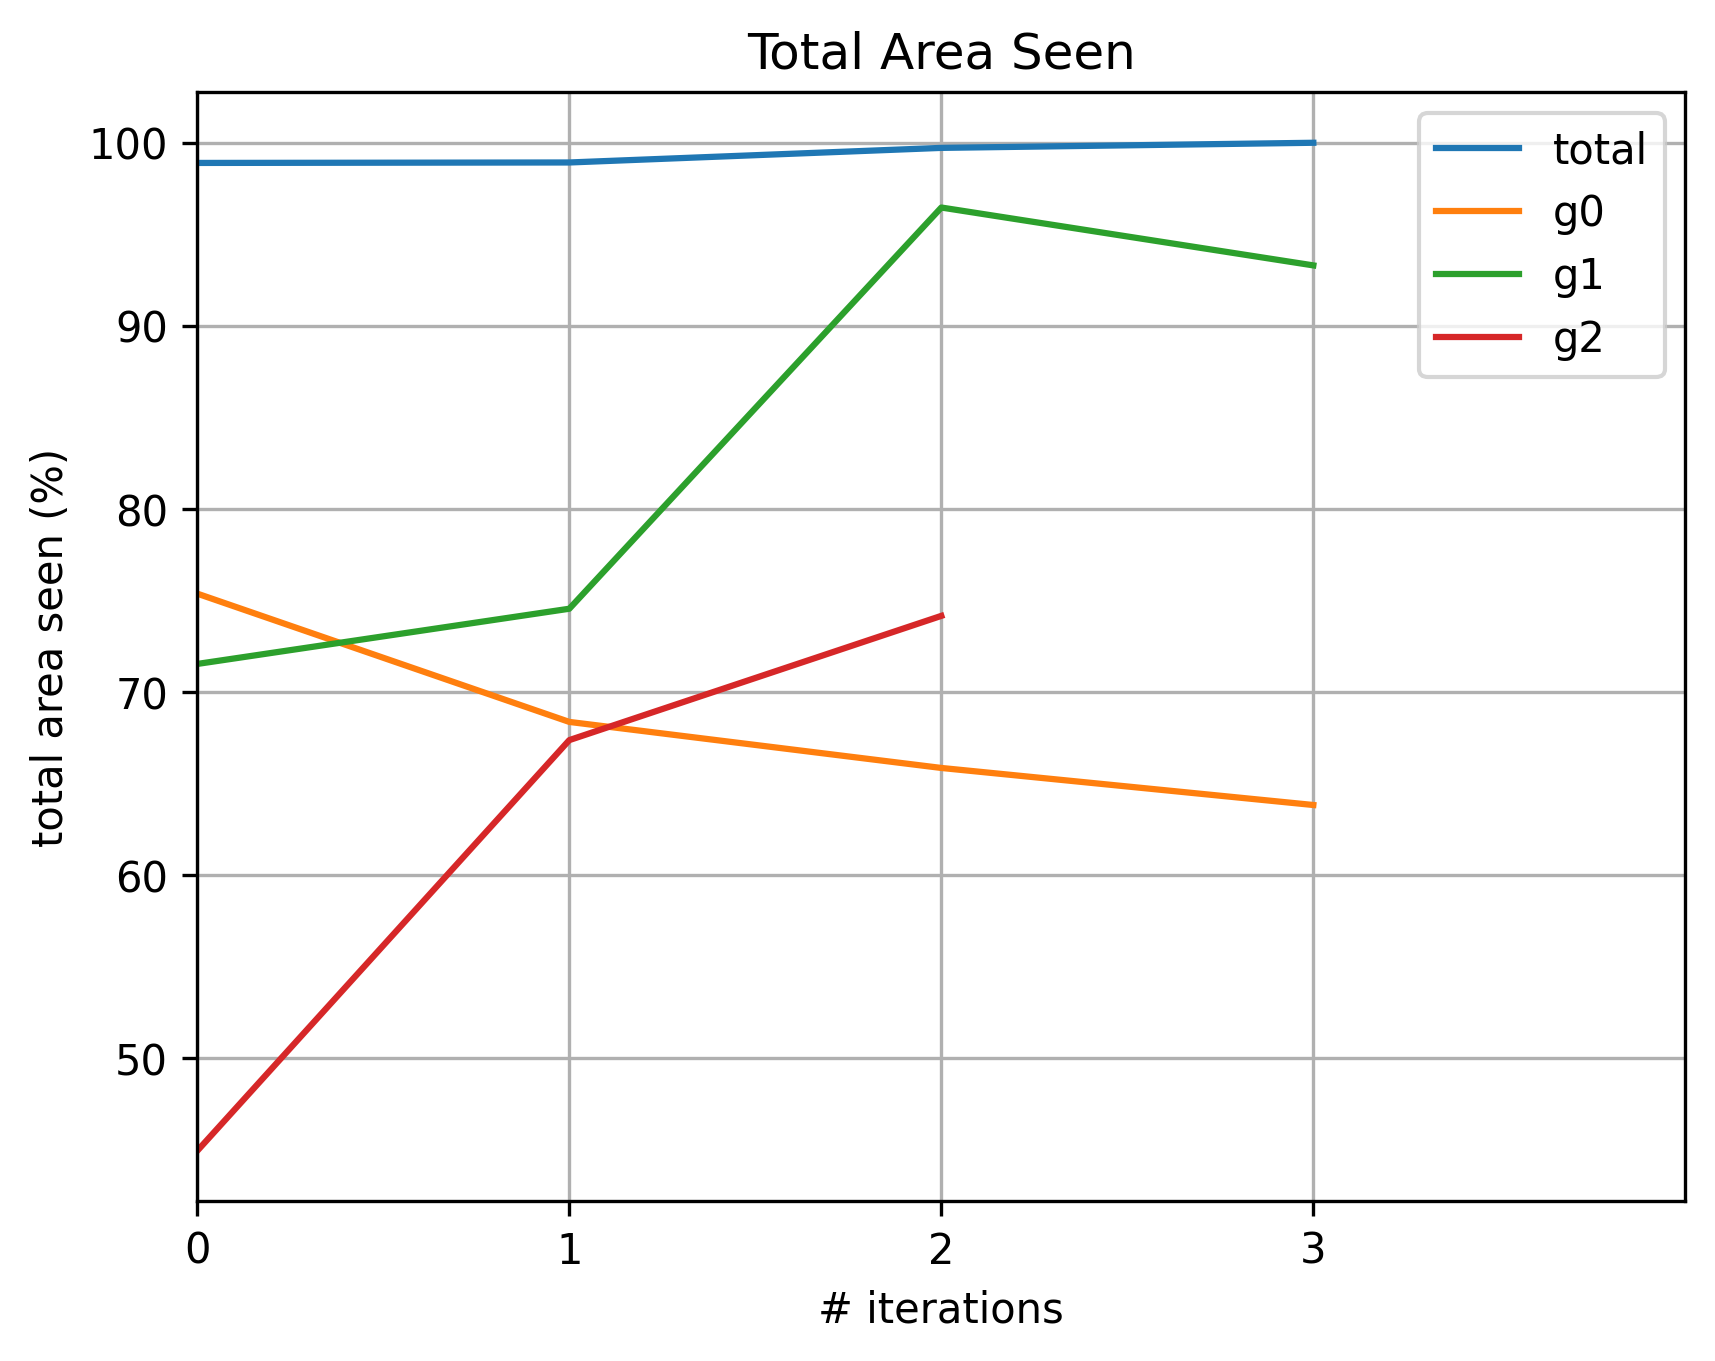
\includegraphics[width = \textwidth]{experiments/area_random_all.png}
        \caption{All heuristics.}
        \label{fig:no_momentum1}
    \end{subfigure}
    \begin{subfigure}{0.45\textwidth}
        \includegraphics[width = \textwidth]{experiments/area_random_no_momentum.png}
        \caption{No momentum.}
        \label{fig:no_momentum2}
    \end{subfigure}
    \caption{Total area seen per iteration for an arbitrary polygon guarded by 3 guards.}
    \label{fig:no_momentum}
\end{figure}

Thus, it becomes clearer how momentum allows the smoothening of noisy guard movements. We reckon that because guards are holding a steadier trajectory, they are more likely to achieve the optimum in less iterations. When not using momentum, the number of iterations increases substantially. Momentum thus is a crucial improving heuristic to our whole algorithm, both in terms of speedup and in the smoothness of the process.

\subsubsection{Without Line Search}
In this section we will discuss the impact line search has on the overall behaviour of the algorithm. As introduced in Section \ref{sec:line_search}, line search determines how far a guard should move towards the direction vector. In this way, it computes the optimal position of a guard on the movement direction given a step size.

For our experiments, we will be using a step size factor of 2. This will allow us to search a larger space of position possibilities knowing the direction of the gradient descent. 
Namely, we will start with a factor of $\frac 1 x$, and we will increase it by a factor of $s$ up to factor $x$. We choose step size factor $s = 2$ and $x = 32$ so that we are able to choose in between 10 positions at every iteration. We will pick the best solution along all the step size based on the largest area increase. 

A suggestive way to observe how well Line Search works is with the comb polygon with four teeth from Figure \ref{fig:comb}. Comb polygons with $n$ teeth require $n$ guards to be guarded. In our case, $n = 4$. We will compare how the guards move when we are using all the heuristics to when we are not using line search. They will start at the same fixed position in both cases.

\begin{figure}[h!]
    \centering
    \includegraphics[width = 0.3\textwidth]{experiments/comb.png}
    \caption{Polygon in the shape of a comb with four teeth.}
    \label{fig:comb}
\end{figure}

Figure \ref{fig:no_line_search} displays the area seen per iteration for the comb polygon with four teeth. Both the total area seen and the individual area seen by each guard are shown. Starting with around 82.5\% total area seen, the global optimum is eventually found. Nonetheless, using line search clearly makes a difference between Subfigures \ref{fig:no_line_search1} and \ref{fig:no_line_search2}. The first noticeable difference is the number of iterations. Using line search allows the guards to find their optimal positions in 3 iterations, with a steady increase in the total area seen. On the other hand, not using line search results in the optimal position to be found in more than 80 iterations. What is more, 3 of the guards seem to have found their optimal position after the $30^{\text{th}}$ iteration, whereas the last 50 iterations are spent on only one guard finding its own.


\begin{figure}[h!]
    \centering
    \begin{subfigure}{0.45\textwidth}
        \includegraphics[width = \textwidth]{experiments/area_comb_easy_all.png}
        \caption{All heuristics.}
        \label{fig:no_line_search1}
    \end{subfigure}
    \begin{subfigure}{0.45\textwidth}
        \includegraphics[width = \textwidth]{experiments/area_comb_no_linear_search.png}
        \caption{No line search.}
        \label{fig:no_line_search2}
    \end{subfigure}
    \caption{Total area seen per iteration for the comb polygon with four teeth, guarded by four guards.}
    \label{fig:no_line_search}
\end{figure}

Therefore, we reckon that line search significantly and more efficiently speeds up the process of finding the optimal position for each guard. In this way, each guard moves faster to its optimal position and avoids creating situations where multiple guards that have found their optimal position have to wait for only one guard to find its own.

\subsubsection{Without Pulling Onto Reflex Vertex}
In this section we will discuss the impact the pull onto the reflex vertex heuristic has on the behaviour of the algorithm. Section \ref{sec:pull_onto} introduced the pulling guards on top of a reflex vertex heuristic. This heuristic tackles the idea that if a guard is ``close enough'' to a reflex vertex, then the locally maximum seen area would be achieved by placing the guard on top of the reflex vertex. We have defined a guard being ``close enough'' to a reflex vertex as closer than two thirds of the minimum distance between any two reflex vertices in the polygon.

We will compare how the guards move when we are using all the heuristics to when we are not pulling them onto reflex vertices. The guards will start at the same fixed position in both cases.

Figure \ref{fig:no_pull} displays the two reflex vertex pull cases: Subfigures \ref{fig:all_pull_pos0} and \ref{fig:all_pull_pos1} show how the green guard movement changes when it is placed onto the reflex vertex; Subfigures \ref{fig:no_pull_pos0} and \ref{fig:no_pull_pos1} show how the guard movement changes when the guard is pulled towards the reflex vertex, but not pulled onto it. We can observe how in Subfigure \ref{fig:all_pull_pos1} the green guard is placed onto the reflex vertex. It then strives to reach the unseen polygon part in the upper left corner. On the other hand, in Subfigure \ref{fig:no_pull_pos1} the guard moved away from the reflex vertex. 
% However, its movement still indicates that it should move back, closer to the reflex vertex it was not placed on. 
These events can also be observed in the two seen area plots in Subfigures \ref{fig:area_all_pull} and Subfigures \ref{fig:area_no_pull}. Clearly, the case when the green guard is not placed on top of the reflex vertex results in more iterations, as seen in Subfigure \ref{fig:area_no_pull}. This is due to the fact that the green guard could not take advantage of the local area maximisation by being placed on the reflex vertex. So, it needs to move around more before finding its optimal path. This is also displayed in how the total area seen lowers and then rises in between iterations 1 and 4. Conversely, Subfigure \ref{fig:area_all_pull} displays how the green guard has quickly moved towards the last part of the polygon that was not yet seen. This resulted in a steady increase in the total seen area.

\begin{figure}[h!]
    \centering
    \begin{subfigure}{0.45\textwidth}
        \includegraphics[width = \textwidth]{experiments/random_all_pull_pos0_fixed.png}
        \caption{All heuristics. The green guard is pulled towards the reflex vertex.}
        \label{fig:all_pull_pos0}
    \end{subfigure}
    \hfill
    \begin{subfigure}{0.45\textwidth}
        \includegraphics[width = \textwidth]{experiments/random_all_pull_pos1_fixed.png}
        \caption{All heuristics. The green guard is onto the reflex vertex.}
        \label{fig:all_pull_pos1}
    \end{subfigure}
    \vfill
    \begin{subfigure}{0.45\textwidth}
        \includegraphics[width = \textwidth]{experiments/random_no_pull_pos0_fixed.png}
        \caption{No pull onto the reflex vertex. The green guard is pulled towards the reflex vertex.}
        \label{fig:no_pull_pos0}
    \end{subfigure}
    \hfill
    \begin{subfigure}{0.45\textwidth}
        \includegraphics[width = \textwidth]{experiments/random_no_pull_pos1_fixed.png}
        \caption{No pull onto the reflex vertex. The green guard is placed according to the momentum computation.}
        \label{fig:no_pull_pos1}
    \end{subfigure}
    \vfill
    \begin{subfigure}{0.45\textwidth}
        \includegraphics[width = \textwidth]{experiments/area_random_all_fixed.png}
        \caption{Seen area for all heuristics.}
        \label{fig:area_all_pull}
    \end{subfigure}
    \hfill
    \begin{subfigure}{0.45\textwidth}
        \includegraphics[width = \textwidth]{experiments/area_random_no_pull_fixed.png}
        \caption{Seen area without pull onto reflex vertices.}
        \label{fig:area_no_pull}
    \end{subfigure}
    \caption{Comparison between a guard being and not being pulled onto a reflex vertex in an arbitrary polygon guarded by four guards.}
    \label{fig:no_pull}
\end{figure}


Therefore, we believe that pulling guards on top of reflex vertices when they are ``close enough'' results in the local maximisation of the area seen by those guards. The number of iterations needed to reach the global maximum is thus reduced. So, the efficiency of the algorithm is also positively affected.

\subsubsection{Without Pull Capping}
In this section we will discuss how not capping the pull towards a reflex vertex influences the overall progression of the guards' movements. Section \ref{sec:pull_capping} introduced the notion of capping the pull towards a reflex vertex. The reason for this choice was to not give the pull the possibility to overpower the value of the momentum. So, if the pull is larger than a factor $\mu$ than the momentum, it is capped at the momentum value of a factor of $\mu$. 

We will compare how the guards move when we are using all the heuristics to when we are not capping the pull towards reflex vertices. We will use the comb polygon with four teeth as example. The guards have a pull cap hyperparameter $\mu = 1$. Thus, if the pull is larger than the momentum, we cap it at the size of the momentum. The reason behind this hyperparameter choice was that it offers a middle ground in between pull capping values that are significantly larger or smaller than the momentum. So, if the pull is as large as the momentum, we will decide to prioritise giving the guard the choice to be pulled onto a reflex vertex if it is ``close enough''.

Figure \ref{fig:no_capping} displays the two reflex vertex pull cases: Subfigures \ref{fig:all_cap_pos0} and \ref{fig:all_cap_pos1} show how the blue guard movement changes when its pull is capped; Subfigures \ref{fig:no_cap_pos0} and \ref{fig:no_cap_pos1} show the opposite. We can observe how in Subfigure \ref{fig:all_cap_pos0} the blue guard has its pull towards the reflex vertex capped. In that case, the pull is not strong enough to move the guard towards the reflex vertex. So, the blue guard moves as its momentum dictates to the position in Subfigure \ref{fig:all_cap_pos1}. This can result in encouraging the guard to explore the polygon more rather than directly moving towards a reflex vertex.
Conversely, Subfigure \ref{fig:no_cap_pos1} displays the blue guard moving closer to the reflex vertex it is pulled to. In subsequent iterations, it is placed on the reflex vertex

Subfigures \ref{fig:area_all_cap} and \ref{fig:area_no_cap} show how the global behaviour of the algorithm is influenced by the capping. Interestingly enough, when capping the pull, the guards' behaviour is more erratic, resulting in more iterations before the whole polygon is seen. On the other hand, using no capping allows a steadier increase in the total area seen. Eventually, the blue guard is drawn and placed onto the reflex vertex. This reinforces the previously discussed idea that placing guards on reflex vertices is beneficial for the overall run of the algorithm. Nonetheless, tuning the hyperparameter $\mu$ is a crucial point of exploration for deciding how and when pull capping would always prove most beneficial.

\begin{figure}[h!]
    \centering
    \begin{subfigure}{0.45\textwidth}
        \includegraphics[width = \textwidth]{experiments/comb_capping_pos0.png}
        \caption{All heuristics. The guard's pull towards the reflex vertex is capped.}
        \label{fig:all_cap_pos0}
    \end{subfigure}
    \hfill
    \begin{subfigure}{0.45\textwidth}
        \includegraphics[width = \textwidth]{experiments/comb_capping_pos1.png}
        \caption{All heuristics. The guard does not act upon the pull towards the reflex vertex.}
        \label{fig:all_cap_pos1}
    \end{subfigure}
    \vfill
    \begin{subfigure}{0.45\textwidth}
        \includegraphics[width = \textwidth]{experiments/comb_no_capping_pos0.png}
        \caption{No pull onto the reflex vertex. The guard's pull towards the reflex vertex is not capped.}
        \label{fig:no_cap_pos0}
    \end{subfigure}
    \hfill
    \begin{subfigure}{0.45\textwidth}
        \includegraphics[width = \textwidth]{experiments/comb_no_capping_pos1.png}
        \caption{No pull onto the reflex vertex. The guard is drawn closer to the reflex vertex.}
        \label{fig:no_cap_pos1}
    \end{subfigure}
    \vfill
    \begin{subfigure}{0.45\textwidth}
        \includegraphics[width = \textwidth]{experiments/area_comb_capping.png}
        \caption{Seen area for all heuristics.}
        \label{fig:area_all_cap}
    \end{subfigure}
    \hfill
    \begin{subfigure}{0.45\textwidth}
        \includegraphics[width = \textwidth]{experiments/area_comb_no_capping.png}
        \caption{Seen area without pull capping.}
        \label{fig:area_no_cap}
    \end{subfigure}
    \caption{Example of different behaviours of a guard with and without its reflex vertex pull capped in a comb polygon with four teeth.}
    \label{fig:no_capping}
\end{figure}

Therefore, we believe that capping the guards' pull towards a reflex vertex highly depends on the hyperparameter $\mu$ and the shape of the polygon. When not capped, it additionally reinforces the importance of placing guards on reflex vertices. However, when the pull of guards is capped, we are using a more exploratory approach to discovering the polygon.

\subsubsection{Without Reflex Area}
In this section we will discuss the importance of keeping guards in the ``reflex area'' of a reflex vertex they've been placed on. Section \ref{sec:reflex_area} introduced this heuristic. The idea is based on the fact that if guards who have been placed on reflex vertices move away from them, they might unsee some of the area they saw when on the reflex vertex. In order to prevent them from looping moving away and then back on the vertex, we will keep them in the reflex area.

We will compare how the guards move when we are using all the heuristics to when we are not keeping guards into a reflex area. We will use another arbitrary polygon as an example.

Figures \ref{fig:reflex_area_eg} and \ref{fig:area_reflex_area} compare using and not using the reflex area heuristic in terms of guard movement and total seen area, respectively. Subfigures \ref{fig:reflex_area_all1} - \ref{fig:reflex_area_all4} show the guards' movement when one of them is bound to the reflex area. In this case, because the blue guard wants to move away from the reflex vertex, the reflex area does not allow it to move away from the reflex vertex. So, it stays there. 
Subfigures \ref{fig:reflex_area_no1} - \ref{fig:reflex_area_no4} display the guards' movement when the reflex area heuristic is not applied. In this case, the blue guard moves away from the reflex vertex (Subfigure \ref{fig:reflex_area_no2}), to be drawn back to it in the next iteration (Subfigure \ref{fig:reflex_area_no3}). This repetitive behaviour continues without allowing the polygon to be completely seen.

\begin{figure}[h!]
    \centering
    \begin{subfigure}{0.45\textwidth}
        \includegraphics[width = \textwidth]{experiments/reflex_area_all_pos3.png}
        \caption{All heuristics. The blue guard is on the reflex vertex.}
        \label{fig:reflex_area_all1}
    \end{subfigure}
    \hfill
    \begin{subfigure}{0.45\textwidth}
        \includegraphics[width = \textwidth]{experiments/reflex_area_all_pos4.png}
        \caption{All heuristics. The blue guard is still on the reflex vertex (in the reflex area).}
    \end{subfigure}
    \hfill
    \begin{subfigure}{0.45\textwidth}
        \includegraphics[width = \textwidth]{experiments/reflex_area_all_pos5.png}
        \caption{All heuristics. The blue guard is still on the reflex vertex (in the reflex area).}
    \end{subfigure}
    \hfill
    \begin{subfigure}{0.45\textwidth}
        \includegraphics[width = \textwidth]{experiments/reflex_area_all_pos6.png}
        \caption{All heuristics. The blue guard is still on the reflex vertex (in the reflex area).}
        \label{fig:reflex_area_all4}
    \end{subfigure}
    \begin{subfigure}{0.45\textwidth}
        \includegraphics[width = \textwidth]{experiments/reflex_area_no_pos4.png}
        \caption{No reflex area. The blue guard is on the reflex vertex.}
        \label{fig:reflex_area_no1}
    \end{subfigure}
    \hfill
    \begin{subfigure}{0.45\textwidth}
        \includegraphics[width = \textwidth]{experiments/reflex_area_no_pos5.png}
        \caption{No reflex area. The blue guard moved away from the reflex vertex.}
        \label{fig:reflex_area_no2}
    \end{subfigure}
    \hfill
    \begin{subfigure}{0.45\textwidth}
        \includegraphics[width = \textwidth]{experiments/reflex_area_no_pos6.png}
        \caption{No reflex area. The blue guard is drawn back to the same reflex vertex.}
        \label{fig:reflex_area_no3}
    \end{subfigure}
    \hfill
    \begin{subfigure}{0.45\textwidth}
        \includegraphics[width = \textwidth]{experiments/reflex_area_no_pos7.png}
        \caption{No reflex area. The blue guard is back on the reflex vertex.}
        \label{fig:reflex_area_no4}
    \end{subfigure}
    \caption{Comparison between using and not using the reflex area heuristic on an arbitrary polygon guarded by two guards.}
    \label{fig:reflex_area_eg}
\end{figure}

Figure \ref{fig:reflex_area_eg} displays the difference in the areas seen between the two approaches. When using all heuristics (Subfigure \ref{fig:area_reflex_area_all}), the algorithm terminates in 7 iteration. The continuous line clearly marks the guard who did not move away from the reflex vertex. When not using the reflex area heuristic (Subfigure \ref{fig:area_reflex_area_no}), the algorithm appears not to terminate. One of the guards loops away and back on the reflex vertex. The other guard loops so that it sees the area that is being seen and unseen by the other guard. In this way, they do not synchronise in order to see the polygon together at the same time.

\begin{figure}[h!]
    \centering
    \begin{subfigure}{0.45\textwidth}
        \includegraphics[width = \textwidth]{experiments/area_reflex_area_all.png}
        \caption{Area seen for all heuristics on another arbitrary polygon.}
        \label{fig:area_reflex_area_all}
    \end{subfigure}
    \hfill
    \begin{subfigure}{0.45\textwidth}
        \includegraphics[width = \textwidth]{experiments/area_reflex_area_no.png}
        \caption{Area seen for no reflex area heuristic on another arbitrary polygon.}
        \label{fig:area_reflex_area_no}
    \end{subfigure}
    \caption{Area comparison between using and not using the reflex area heuristic on an arbitrary polygon guarded by two guards.}
    \label{fig:area_reflex_area}
\end{figure}

Therefore, we believe that the reflex area heuristic is of great importance to the correct run of the algorithm. It addresses the issue of guards moving away and back on reflex vertices. This behaviour causes the other guards to move towards the area that becomes unseen by the first guard. In this way, the guards continue to move out of sync with each other, resulting in the polygon never being fully seen.

\subsubsection{No Hidden Gradient}
In this section we will discuss the importance of using a hidden gradient heuristic. Section \ref{sec:hidden_gradient} introduced this heuristic. The idea is based on the fact that we want guards to make progress, no matter how little. If a guard's visibility region is already seen by other guards, it is unlikely that its position is optimal. Thus, we want the guard to still move.

We will compare how the guards move when we are using all the heuristics to when we are not moving guards when their visibility region is fully seen by other guards. We will use the comb polygon with four teeth as an example. 

Figure \ref{fig:area_no_hidden_gradient} displays a comparison between using and not using hidden gradient in our algorithm. In Subfigure \ref{fig:area_comb_no_hidden_gradient} we can notice that the execution of the algorithm takes twice as many iterations than in Subfigure \ref{fig:area_comb_all2}. The reason behind this is the fact that for half of the iterations two of the guards do not move when no hidden gradient is used. Additionally, the total area seen in that case fluctuates. This is in contrast with the case where the hidden gradient heuristic is used. In that case, the total area seen is continuously increasing, and all guards who can make progress move.

\begin{figure}[h!]
    \centering
    \begin{subfigure}{0.45\textwidth}
        \includegraphics[width = \textwidth]{experiments/area_comb_all.png}
        \caption{All heuristics.}
        \label{fig:area_comb_all2}
    \end{subfigure}
    \begin{subfigure}{0.45\textwidth}
        \includegraphics[width = \textwidth]{experiments/area_comb_no_hidden_gradient.png}
        \caption{No hidden gradient.}
        \label{fig:area_comb_no_hidden_gradient}
    \end{subfigure}
    \caption{Seen area for the comb polygon with four teeth guarded by four guards.}
    \label{fig:area_no_hidden_gradient}
\end{figure}

Therefore, we believe that the hidden gradient heuristic results in a significant improvement to our algorithm in terms of efficiency. In this way, all guards are ensured to make some progress towards their optimum and are not stalled.

\subsubsection{Without Angle Behind Reflex Vertex}
In this section we will discuss the benefits of using the value of the angle behind reflex vertices. Section \ref{sec:angle} introduced this heuristic. The idea behind this technique is that guards should be drawn faster to larger unseen areas behind reflex vertices. Conversely, if the unseen area behind the reflex vertex is very small, we also want guards to move towards it. In this way, we prioritise unseen areas based on their size, while still accounting for the very small unseen areas.

Figure \ref{fig:no_angle} shows a comparison between using and not using the angle behind the reflex vertex heuristic: Subfigures \ref{fig:all_angle_pos0} and \ref{fig:all_angle_pos1} display the first two iterations of the algorithm when all heuristics are used, whereas  Subfigures \ref{fig:no_angle_pos0} and \ref{fig:no_angle_pos1} focus on the first two iterations when not using the angle behind the reflex vertex.
We can observe a major difference in the way the final momentum movement is computed for the orange guard in the two cases. When all heuristics are used, the movements of the guards are much smaller and calculated than when the angle does not play a role. For example, in Subfigure \ref{fig:no_angle_pos0}, the orange guard has a very large momentum movement outside of the polygon due to the unseen part in the upper pocket. When we also take into account the angles behind the reflex vertices in the pocket, its movements become much smaller (Subfigure \ref{fig:all_angle_pos0}). In fact, the orange guard is also drawn slightly the right part of the polygon, as it has a larger angle behind the reflex vertex. That part of the polygon is already seen by the blue guard, so it starts moving towards the upper pocket in Subfigure \ref{fig:all_angle_pos1}.

In terms of efficiency, the optimal solution is achieved in more iterations when the movements of the guards when the angle heuristic is used. This can be observed in Subfigures \ref{fig:area_all_angle} and \ref{fig:area_no_angle}. When using all heuristics, the random polygon is fully seen in 5 iterations. The movement of the guards is smooth. Two of the guards have an increasing seen area, whereas the orange guard moves slowly towards the upper pocket of the polygon. Not using the angle heuristic allows us to achieve the same goal in only 3 iterations. As mentioned, the progress of the guards is not as smooth.


\begin{figure}[h!]
    \centering
    \begin{subfigure}{0.45\textwidth}
        \includegraphics[width = \textwidth]{experiments/random_all_pull_pos0_fixed.png}
        \caption{All heuristics. The orange guard's movement is towards upper right.}
        \label{fig:all_angle_pos0}
    \end{subfigure}
    \hfill
    \begin{subfigure}{0.45\textwidth}
        \includegraphics[width = \textwidth]{experiments/random_all_pull_pos1_fixed.png}
        \caption{All heuristics. The orange guard's movement is towards upper left.}
        \label{fig:all_angle_pos1}
    \end{subfigure}
    \vfill
    \begin{subfigure}{0.45\textwidth}
        \includegraphics[width = \textwidth]{experiments/random_no_angle_pos0.png}
        \caption{No angle behind the reflex vertex. The orange guard's movement is all the way to the left boundary of the polygon.}
        \label{fig:no_angle_pos0}
    \end{subfigure}
    \hfill
    \begin{subfigure}{0.45\textwidth}
        \includegraphics[width = \textwidth]{experiments/random_no_angle_pos1.png}
        \caption{No angle behind the reflex vertex. The orange guard's movement is towards the left-side outside of the polygon.}
        \label{fig:no_angle_pos1}
    \end{subfigure}
    \vfill
    \begin{subfigure}{0.45\textwidth}
        \includegraphics[width = \textwidth]{experiments/area_random_all_fixed.png}
        \caption{Seen area for all heuristics.}
        \label{fig:area_all_angle}
    \end{subfigure}
    \hfill
    \begin{subfigure}{0.45\textwidth}
        \includegraphics[width = \textwidth]{experiments/area_random_no_angle.png}
        \caption{Seen area without the angle behind the reflex vertices.}
        \label{fig:area_no_angle}
    \end{subfigure}
    \caption{Comparison between using and not using the angle behind a reflex vertex in an arbitrary polygon guarded by three guards.}
    \label{fig:no_angle}
\end{figure}

Therefore, we believe that computing the angle behind the reflex vertex is a heuristic that allows us to fine-tune and smoothen the movement of the guards. In this way, we can focus on moving fast towards the bigger unseen areas, while also not neglecting the smaller ones. We could say that this heuristic offers a trade-off between the number of iterations and path smoothness. For this reason, we believe that the performance of the algorithm is influenced by the type of polygons it is applied to: polygons with sharper, narrower turns could benefit the most from this heuristic.

\subsubsection{Greedy Initialisation}
In this section we will discuss the benefits of using a greedy initialisation technique for our algorithm. Section \ref{sec:greedy} introduces this heuristic as beneficial for giving a head start to our algorithm. In our experiments we will greedily initialise the guards in the middle of the leftmost segment of each of their visibility regions. The reason behind this choice is that CGAL did not offer a quick way to pick a randomised position inside the visibility area. Due to the time constraints of this thesis, we decided to use a deterministic positioning.

So far we have not used greedy initialisation in any of our examples. The reason is that this technique can already solve some polygons at guard placement time. Naturally, this would not allow us to show the benefits of using any of the other heuristics. An example in this case is the comb polygon with four teeth in Figure \ref{fig:comb_greedy}.

\begin{figure}[h!]
    \centering
    \includegraphics[width = 0.7\textwidth]{experiments/comb_greedy.png}
    \caption{The comb polygon with four teeth is already completely seen at greedy initialisation time.}
    \label{fig:comb_greedy}
\end{figure}

In the case of polygons who are not completely seen at initialisation time, it is unclear whether the greedy placement improves the overall progress. How well the algorithm behaves is highly dependent on the initial placement of the guards. Namely, the algorithm often does not finish with different starting positions (it is stuck in local optima). Because of this drawback, we cannot create extensive experiments with different starting guard positionings. It is additionally not feasible to find a generalisation in the type of placements that allow the algorithm to finish.

Therefore, we believe a randomised placement of the guards during the greedy initialisation would be beneficial for giving a head start to the algorithm. However, due to time constraints, this heuristic is to be explored more with a more robust algorithm implementation.
% - momentum
% - reflex vertex pull
    % - onto reflex vertex
    % - pull Capping
% - line search
% - reflex area
% - hidden gradient
% - angle behind reflex vertex
% - greedy initialisation

\subsection{Scaling for the Comb Polygon}
In this section we will observe how the algorithm scales on the comb polygon. We will take the comb polygons with 2, 3, ..., 10, 15, 20, 50, 100 teeth. We will note how the algorithm progresses in terms of the total area seen per iteration.
As such, we will run the algorithm with all heuristics for all the previously mentioned comb polygons. All guards will start at the same $y$-coordinate, 0.1 units apart from each other. An example of such a starting point can be found in Figure \ref{fig:comb6_start_pos}. In this way, we can ensure that the performance of the algorithm can be compared using the same starting position of the guards. We will deem a timeout of two hours for declaring an algorithm unfeasible for larger polygons. We will then analyse how the algorithm performed under each of the circumstances. Lastly, we will offer some points of improvement.

\begin{figure}[h!]
    \centering
    \includegraphics[width = 0.7\textwidth]{experiments/comb6_start_pos.png}
    \caption{In the comb polygon with 6 teeth, all guards start at the same $y$-coordinate, with 0.1 units in between them.}
    \label{fig:comb6_start_pos}
\end{figure}

We expect that the number of iterations needed would scale with the number of teeth of the polygon. We are also interested in how the execution time would scale. We expect that the time limit would already be achieved with less than 20 comb teeth.

Figure \ref{fig:all_combs} display the progression of our algorithm for the comb polygons with 2, 3, ..., 10, 15, 20 teeth within one hour. The comb polygons with 50 and 100 teeth did not complete any iteration within that time.
For comb polygons with 5 teeth and more than 6 teeth, the timeout was not enough to find a feasible solution. Nonetheless, it is worth discussing their behaviour, as it highlights the different issues the algorithm faces. 
For comb polygons with 7, 9 and 10 teeth, the guards appear to be stuck in a local plateau that it did not manage to escape. This can be traced to an edge case where the guards are stuck in their position because their movement vector does not improve the total area. Another reason why the guards do not move is that they are still trying to maximise their local viewed area in the case where the total area seen cannot be increased within that step. This could result in them all moving to the same part of the polygon. Since that part of the polygon maximises their locally seen area, they will not move anymore.
For comb polygon with 5 teeth, the guards appear to be stuck in a local maxima that they manage to escape. Unfortunately, they later return to it and restart the cycle. It is unclear whether the comb polygon with 8 teeth would display a similar looping behaviour. Given the timeout, the guards trying to solve the comb polygon with 8 teeth display a less predictable behaviour. We believe that hyperparameter tuning could address this issue.

\begin{figure}[h!]
    \centering
    \includegraphics[width = \textwidth]{experiments/all_combs_areas.png}
    \caption{The percentage of the area seen in terms of iterations for comb polygons with 2, 3, ..., 10, 15, and 20 teeth.}
    \label{fig:all_combs}
\end{figure}

Conversely, it is also crucial to address the comb polygons which the algorithm manage to solve: 2, 3, 4 and 6 teeth. In this case, we can observe a clear scaling: the more teeth a comb polygon has, the longer it takes to be solved. What is more, the solution also scales with the number of teeth. The comb polygon with 4 and 6 teeth take twice as many iterations to be solved than the ones with 2 and 3 teeth, respectively. We would expect a similar behaviour for comb polygons with more teeth, if the algorithms would finish.

\begin{figure}[h!]
    \centering
    \includegraphics[width = \textwidth]{experiments/good_combs_areas.png}
    \caption{The percentage of the area seen in terms of iterations for comb polygons with 2, 3, 4, and 6 teeth.}
    \label{fig:good_combs}
\end{figure}

It is worth discussing how the initial guard placement and comb polygon shapes could influence the performance of the algorithm.
Firstly, it is importance to discuss the initial placement strategy. Guards are placed in the same lower left part of the polygon. However, the larger a polygon, the lower the initially seen area. For example, we can observe how the comb polygon with 2 teeth starts at more than 80\% seen area. On the other hand, the comb polygon with 20 teeth has a less than 65\% seen area at start. We could argue that this gives larger polygons a start disadvantage.
Moreover, the algorithm is sensitive to the shape of the polygons. The bigger a comb polygon grows, the sharper and narrower its teeth are. A good example in this case is Figure \ref{fig:comb20}, which displays a comb polygon with 20 teeth. Clearly, the teeth are much narrower than in the case of a comb with 4 teeth. This raises the question about the role the shape of the teeth plays into the algorithm performing better or worse. A possible solution to this aspect would be to scale up the polygon. However, a similar question would remain: does the algorithm necessarily perform better or worse because of the polygon shape? and what would be the optimal such shape?

\begin{figure}[h!]
    \centering
    \includegraphics[width = 0.8\textwidth]{experiments/comb20.png}
    \caption{Comb polygon with 20 teeth.}
    \label{fig:comb20}
\end{figure}

\subsection{Hyperparameter Sensitivity}
\label{sec:hyperparameters}
The algorithm is highly sensitive to the hyperparameter choices, polygons shapes and sizes, and guard starting points. We have already emphasised how the hyperparameter values have been chosen: other values than the ones used would result in the program crashing on not terminating. Similarly, in the context of the comb polygon, we have discussed that the polygon shape can have a crucial effect on the performance of the algorithm.

In this section we will additionally explain how the guard starting points influence the outcome of the program. We will use the irrational guards polygon \cite{abrahamsen2021art} as an example.
The polygon can be guarded by 3 guards with irrational coordinates, or 4 guards with rational coordinates. We will thus compare these types of positionings. We will place 3 guards at an approximation of the irrational coordinates, and 4 guards at arbitrary rational coordinates. The approximated irrational guards will have coordinates $(2, 0.59), (19, 1.71), (10.57, 2.12)$. The arbitrary guards will have coordinates $(5, 0), (5.5, 0), (6, 0), (6.5, 0)$.

Figure \ref{fig:irrational} displays the difference in runs between the previously mentioned guard placements. The orange line displays the algorithm run for the guard irrational approximation coordinates. As expected, the algorithm deems that the whole polygon is seen within the first iteration. On the other side, the blue line shows the algorithm performance for the guards with rational coordinates. Unfortunately, the program in this case crashes after the 8th iteration. The error was unclear and the time constraints of this thesis did not allow us to solve it.

\begin{figure}[!h]
    \centering
    \includegraphics[width = 0.7\textwidth]{experiments/irrational_areas.png}
    \caption{Comparison for the irrational guards polygon between guards with approximately irrational coordinates and rational guard coordinates.}
    \label{fig:irrational}
\end{figure}

Therefore, we believe that the irrational guards polygon is a suggestive example to the sensitivity of the algorithm to initial guard placements. The starting position of the guards can determine whether the algorithm is able to escape local minima or not crash.

\section{Problems Encountered}
The development of this algorithm has encountered a number of important problems that affected its progress.

A large number of issues were posed by the CGAL library itself, due to its non-detailed errors and lack of explicit documentation. Having to reverse engineer and delve into the source-code of CGAL slowed down the debugging process. Because some errors were not explicit at all, some crashes remained unsolved (for example, the program crashes for certain starting positions for different polygons).

Because of the impeded progress, the program is only able to work with a very limited range of simple polygons depending on the heuristics used and the values of the hyperparameters. Some of the polygons the algorithm can solve under the tested circumstances include those mentioned in Section \ref{sec:experiments}. The irrational guards polygon can only be solved if the irrational guards are already very close to the optimum. Polygons from the APGlib library \cite{art-gallery-instances-page} have also been tested. However, the program always gets stuck with them.

The program does not scale. For comb polygons with more than 6 teeth, the waiting time already exceeds an hour to finish.
% - cryptic CGAL errors
% - can only work with simple polygons
% - except for the few test polygons (2 guards, random, comb), all the other testbeds (Simon's) don't work because the algorithm gets stuck/crashes
% - for bigger polygons (more guards) it becomes slow very fast (unfeasible)
- initial guard placement


\section{Further Progress}
- improve the efficiency of the code
    - can add a flag for guards whose gradient has been computed instead of copying the vector
- find a more efficient way of coding to tackle the edge-cases
- implement an expiry date for the reflex area
- implement algorithm for love polygon - currently crashes 
- init gradient is not randomised
\section{Discussion}
This thesis focussed on implementing and evaluating a gradient descent algorithm to find a solution to the Art Gallery Problem. This goal has been achieved for the few discussed polygons. 
Nonetheless, this method raised quite some issues. For this reason, we discussed more in-depth the development process and the performance of the algorithm. There were numerous edge-cases to be taken into account. For many of them, we created various hyperparameterised heuristics. Other heuristics (such as momentum) were created as an improvement to the shortcomings of gradient descent.
% Gradient descent is quite a straight-forward approach. 

The resulting program is sensitive to hyperparameter choices, polygon shapes and starting guard positions. For this reason, we only provided qualitative evaluations for the heuristics used to extend gradient descent. Namely, we discussed both specific added benefits of each of the heuristics, and a comparison based on the average number of iterations required to fully see a polygon. The way this was done is by running the program with all heuristics but the one whose practicality we are discussing. In this way, we assess the added advantage of each heuristic in its absence. The reason behind this experimental setup is that combinations of all heuristics are both verbose and unnecessary. Given that the program is still limited to a few examples, we cannot use extensive statistical tools to test its overall performance. With the given examples, we managed to assess that using the pull heuristic is likely to be statistically significant to improve the algorithm's performance in terms of the number of iterations.
In this way, we provided a pragmatic overview to the usefulness of each of the heuristics and hyperparameters used. Namely, we analysed on what the type of polygons different heuristics and hyperparameter values provide concrete results.

Section \ref{sec:future} further discusses how the program could be improved in the future.



% - evaluation of what I did
%     - selection of heuristics that make sense (because their combination is too long)
% - "conclusion"

\subsection{Future Work}
\label{sec:future}
Currently, the program offers a state-of-the-art view about its practical possibilities.
In the future, it would be suitable to extend it with more robust functionalities.

One of the most crucial aspects of improvement for the program would be to solve the existing errors and bugs. As of now, the program crashes for specific input polygons (see Section \ref{sec:problems} for an extensive overview of its shortcomings). Another important element to consider would be to code it more efficiently, as the program does not scale. This is because some of the data structures and techniques used are naive (brute-forced). Implementing them in a more efficient way should improve the scalability of the program.

Additionally, some features and heuristics are not complete. For example, the greedy initialisation of the guards' position is deterministic. In order to quantitatively assess the performance of the algorithm, a truly randomised greedy initialisation would be required for statistical significance.

Lastly, it would be worth exploring how the algorithm would benefit from a different implementation. Namely, using another programming language like Python (or CGAL Python bindings) and other geometry libraries which are better documented and more reliable to use.
% - improve the efficiency of the code
%     - can add a flag for guards whose gradient has been computed instead of copying the vector
% - find a more efficient way of coding to tackle the edge-cases
% - implement an expiry date for the reflex area
% - implement algorithm for love polygon - currently crashes 
% - init gradient is not randomised -> should do that for finding actually working starting positions
% - give an impression on the code improvement


\newpage
\thispagestyle{empty}
\section*{Acknowledgements}
I would like to thank Till Miltzow and Frank Staals for supervising the thesis and always offering creative and constructive feedback. I would also like to thank Simon Hengeveld for the helpful advice and explanation of his implementation for solving the Art Gallery Problem.
Lastly, I would like to thank my partners Tim and Teun for always supporting me during both the rough and the happy times of this thesis.
\printbibliography

\renewcommand{\headrulewidth}{0pt}% Remove header rule
\fancyhead{}% Remove all header contents

% \bibliographystyle{unsrt}

%\include{3_Appendix}


\end{document}